
% ----------------------------------------------------------------------
%                   Latex File for Eamon O'Gorman's PhD (2013)
% ----------------------------------------------------------------------

%Latext thesis template from Harish Bhanderi's PhD/MPhil template, then Uni Cambridge
% http://www-h.eng.cam.ac.uk/help/tpl/textprocessing/ThesisStyle/

%: Style file for Latex
% Most style definitions are in the external file PhDthesisPSnPDF.
% In this template package, it can be found in ./Latex/Classes/
\documentclass[a4paper, oneside,12pt]{Latex/Classes/PhDthesisPSnPDF}

%Change "oneside" to "twoside" for final submission-grade thesis after viva/corrections

\usepackage{lineno}
\usepackage{amsbsy}
\usepackage{xspace}
\usepackage{wtmmPkg}
\usepackage{natbib}
\usepackage{multirow}
\usepackage{paralist}
\usepackage{titlesec}
\usepackage{lscape}
\usepackage{quotchap}
\usepackage{epstopdf}
\usepackage{fancyhdr}
\usepackage{graphicx}
\usepackage{amsmath}
\usepackage{float}
\usepackage{afterpage}

%Added by SM 13 Sep 2011 to get backref to read ''Cited on page''
   \usepackage{Latex/StyleFiles/backrefx}
       \renewcommand{\backrefpagesname}{Cited on page~}
       \renewcommand{\backrefpagesnames}{Cited on pages~}

\newcommand{\BibTeX}{\textsc{Bib}\TeX}
\newcommand{\etal}{{\it et al.}}

% Definitions for equations
\newcommand{\arcsec}{^{\prime\prime}}
%\def\ion#1#2{#1$\;${\small\rm\@Roman{#2}}\relax}
\DeclareRobustCommand{\ion}[2]{%
\relax\ifmmode
\ifx\testbx\f@series
{\mathbf{#1\,\mathsc{#2}}}\else
{\mathrm{#1\,\mathsc{#2}}}\fi
\else\textup{#1\,{\mdseries\textsc{#2}}}%
\fi}

\newcommand{\subion}{ {_{ion}} }
\newcommand{\sube}{ {_{e}} }
\newcommand{\subj}{ {_{j}} }
\newcommand{\subi}{ {_{i}} }
\newcommand{\ji}{ {_{j,i}} }
\newcommand{\rt}{ {$R(T)$} }
\newcommand{\rlam}{ {$R(\lambda)$} }
\newcommand{\rsun}{R$_{\odot}$}
\newcommand{\rmd}{ {\ \mathrm d} }
\renewcommand{\vec}[1]{ {\mathbf #1} }
\newcommand{\uvec}[1]{ \hat{\mathbf #1} }
\newcommand{\pder}[2]{ \f{\partial #1}{\partial #2} }
\newcommand{\grad}{ {\bf \nabla } }
\newcommand{\curl}{ {\bf \nabla} \times}
\newcommand{\vol}{ {\mathcal V} }
\newcommand{\bndry}{ {\mathcal S} }
\newcommand{\dv}{~{\mathrm d}^3 x}
\newcommand{\da}{~{\mathrm d}^2 x}
\newcommand{\dl}{~{\mathrm d} l}
\newcommand{\dt}{~{\mathrm d}t}
\newcommand{\intv}{\int_{\vol}^{}}
\newcommand{\inta}{\int_{\bndry}^{}}
\newcommand{\avec}{ \vec A}
\newcommand{\ap}{ \vec A_p}
\newcommand{\bb}{ \vec B}
\newcommand{\jj}{ \vec j}
\newcommand{\rr}{ \vec r}
\newcommand{\xx}{ \vec x}

% Definitions for the journal names
\newcommand{\adv}{    {\it Advances in Space Research}}
\newcommand{\annG}{   {\it Annales Geophysicae}}
\newcommand{\aap}{    {\it Astronomy \& Astrophysics}}
\newcommand{\aaps}{   {\it Astronomy \& Astrophysics Supplemental}}
\newcommand{\aapr}{   {\it Astronomy \& Astrophysics Review}}
\newcommand{\ag}{     {\it Ann. Geophys.}}
\newcommand{\aj}{     {\it Astronomical Journal}}
\newcommand{\apj}{    {\it Astrophysical Journal}}
\newcommand{\apjs}{    {\it Astrophysical Journal Supplemental Series}}
\newcommand{\apjl}{   {\it Astrophysical Journal Letters}}
\newcommand{\apss}{   {\it Astrophysics \& Space Science}}
\newcommand{\cjaa}{   {\it Chinese Journal Astronomy \& Astrophysics}}
\newcommand{\gafd}{   {\it Geophysical and Astrophysical Fluid Dynamics}}
\newcommand{\grl}{    {\it Geophysical Research Letters}}
\newcommand{\ijga}{   {\it International Journal of Geomagnetism and Aeronomy}}
\newcommand{\jastp}{  {\it Journal of Atmospheric and Solar-Terrestrial Physics}}
\newcommand{\jgr}{    {\it Journal of Geophysical Research}}
\newcommand{\mnras}{  {\it Monthly Notices of the Royal Astronomical Society}}
\newcommand{\nat}{    {\it Nature}}
\newcommand{\pasp}{   {\it Publications of the Astronomical Society of the Pacific}}
\newcommand{\pasj}{   {\it Publications of the Astronomical Society of Japan}}
\newcommand{\pra}{    {\it Physical Review A}}
\newcommand{\pre}{    {\it Physical Review E}}
\newcommand{\solphys}{{\it Solar Physics}}
\newcommand{\sovast}{ {\it Soviet Astronomy}}
\newcommand{\ssr}{    {\it Space Science Reviews}}
\newcommand{\araa}{  {\it Annual Review of Astronomy \& Astrophysics}}
\newcommand{\memsai}{ {\it Memorie della Societa Astronomia Italiana}}

%: Macro file for Latex
% Macros help you summarise frequently repeated Latex commands.
% Here, they are placed in an external file /Latex/Macros/MacroFile1.tex
% An macro that you may use frequently is the figuremacro (see introduction.tex)
% This file contains macros that can be called up from connected TeX files
% It helps to summarise repeated code, e.g. figure insertion (see below).

% insert a centered figure with caption and description
% parameters 1:filename, 2:title, 3:description and label
\newcommand{\figuremacro}[3]{
	\begin{figure}[htbp]
		\centering
		\includegraphics[width=1\textwidth]{#1}
		\caption[#2]{\textbf{#2} - #3}
		\label{#1}
	\end{figure}
}

% insert a centered figure with caption and description AND WIDTH
% parameters 1:filename, 2:title, 3:description and label, 4: textwidth
% textwidth 1 means as text, 0.5 means half the width of the text
\newcommand{\figuremacroW}[4]{
	\begin{figure}[htbp]
		\centering
		\includegraphics[width=#4\textwidth]{#1}
		\caption[#2]{\textbf{#2} - #3}
		\label{#1}
	\end{figure}
}

% inserts a figure with wrapped around text; only suitable for NARROW figs
% o is for outside on a double paged document; others: l, r, i(inside)
% text and figure will each be half of the document width
% note: long captions often crash with adjacent content; take care
% in general: above 2 macro produce more reliable layout
\newcommand{\figuremacroN}[3]{
	\begin{wrapfigure}{o}{0.5\textwidth}
		\centering
		\includegraphics[width=0.48\textwidth]{#1}
		\caption[#2]{{\small\textbf{#2} - #3}}
		\label{#1}
	\end{wrapfigure}
}

% predefined commands by Harish
\newcommand{\PdfPsText}[2]{
  \ifpdf
     #1
  \else
     #2
  \fi
}

\newcommand{\IncludeGraphicsH}[3]{
  \PdfPsText{\includegraphics[height=#2]{#1}}{\includegraphics[bb = #3, height=#2]{#1}}
}

\newcommand{\IncludeGraphicsW}[3]{
  \PdfPsText{\includegraphics[width=#2]{#1}}{\includegraphics[bb = #3, width=#2]{#1}}
}

\newcommand{\InsertFig}[3]{
  \begin{figure}[!htbp]
    \begin{center}
      \leavevmode
      #1
      \caption{#2}
      \label{#3}
    \end{center}
  \end{figure}
}


%%% Local Variables: 
%%% mode: latex
%%% TeX-master: "~/Documents/LaTeX/CUEDThesisPSnPDF/thesis"
%%% End: 


%Change this if compiling at home/office
%\graphicspath{{/Users/josephroche/Work/log_of_learning/images/}}
\graphicspath{{images/}}


%: --------------------------------------------------------------
%:                  FRONT MATTER: dedications, abstract,..
% --------------------------------------------------------------

\usepackage{setspace}
\singlespacing

\begin{document}

\renewcommand\baselinestretch{1.2}
\baselineskip=18pt plus1pt

%: ----------------------- COVER PAGE ------------------------

\newcommand{\titlefont}{\bfseries \fontsize{22}{26.42pt}\selectfont}
\newcommand{\largetitlefont}{\bfseries \fontsize{29.88}{35.88pt}\selectfont}
\newcommand{\othertitlefont}{\fontsize{14.4}{17.28}\selectfont}
\newcommand{\authorfont}{\bfseries \fontsize{14.4}{17.28}\selectfont}
\newcommand{\informationfont}{\fontsize{10}{12}\selectfont}
\newcommand{\dedicationfont}{\slshape \fontsize{14.4}{17.28}\selectfont}

\newcommand{\thisyear}{\number\year}
\def\thismonth{\ifcase\month\or January\or February\or March\or
  April\or May\or June\or July\or August\or September\or October\or November\or December\fi}
\newcommand{\todaysdate}{\thismonth\space \thisyear}

\renewcommand{\baselinestretch}{1}
\newpage \thispagestyle{empty}
\vspace*{1.5cm}
\begin{flushright}


%TITLE

\Huge{\textbf{Radio Interferometric Studies of Cool Evolved Stellar Outflows}}

\end{flushright}

\vspace*{4cm}
\begin{flushright}
A dissertation submitted to the University of Dublin \\
for the degree of Doctor of Philosophy
\end{flushright}

\vspace*{\fill}
\begin{flushright}
{\authorfont Eamon O'Gorman} \\[1mm]
Supervisor: Dr. Graham M. Harper\\[.5mm]
Trinity College Dublin, September 2013\\[.5mm]
\rule{0.9\textwidth}{0.5mm}\\[4mm]

\begin{minipage}[b][15mm][t]{12.5cm}
\raggedleft \sc
School of Physics\\
University of Dublin\\
Trinity College\\
\end{minipage}
\hspace*{1mm}
\begin{minipage}[b][15mm][t]{1.15cm}

\includegraphics[height=16mm]{tcd_crest.eps}
\end{minipage}

 \end{flushright}

%: ----------------------- tie in front matter ------------------------


\frontmatter

%!TEX root = ../thesis.tex
%Adding the above line, with the name of your base .tex file (in this case "thesis.tex") will allow you to compile the whole thesis even when working inside one of the chapter tex files


\begin{declaration}      

I declare that this thesis has not been submitted as an exercise for a degree at this or
any other university and it is entirely my own work.

\vspace{10mm}

I agree to deposit this thesis in the University's open access institutional repository or
allow the library to do so on my behalf, subject to Irish Copyright Legislation and
Trinity College Library conditions of use and acknowledgement.

\vspace{30mm}

\textbf{Name:} Your Name	

\vspace{15mm}

\textbf{Signature:}  ........................................		\textbf{Date:}  ..........................



\end{declaration}

\newpage
\thispagestyle{empty}
\mbox{}


% ----------------------------------------------------------------------


%!TEX root = ../thesis.tex
%Adding the above line, with the name of your base .tex file (in this case "thesis.tex") will allow you to compile the whole thesis even when working inside one of the chapter tex files

\begin{abstracts} 

Mass-loss becomes significant for most stars as they approach the end of their lives and become either red giants or red supergiants. This continuous mass-loss, which occurs in the form of a relatively dense and slow-moving wind, can have a significant impact on the evolution of gas and dust in galaxies, on surrounding planets, and indeed on the very evolution of the star itself.  Despite the importance of this phenomenon and decades of study,
the fundamental mechanisms responsible for producing these winds remain unknown. The main reason for this is due to our lack of understanding of the dynamics and thermodynamics of the stellar outflow environment. Isolated giants and supergiants do not contain the expected additional complexities encountered by binaries, making them ideal targets for understanding the nature of these outflows. Traditionally, observations have provided only limited disk-averaged information about the outflow environments of these stars making it difficult to infer the outflow properties. However, the latest suite of radio interferometers now have the capability to provide essential spatial information on these outflow environments.

This thesis first presents the results of a radio interferometric study into the dynamics of the two unique flows in the circumstellar environment of the  M2 red supergiant, Betelgeuse. The  Combined Array for Research in Millimeter-wave Astronomy (CARMA) was used in multiple configurations to observe the CO($J=2-1$) emission line allowing  spatial scales as small as 0$\arcsec$.9 to be traced over a 32$\arcsec$  field of view. The outer flow known as S2, was found to have outflow velocities of -15.4 and and +13.2 km s$^{-1}$ with respect to the stellar rest frame and extend out to 17$\arcsec$, while the inner flow known as S1, was found to have outflow velocities of -15.4 and and +13.2 km s$^{-1}$ and extend out to $4 \rightarrow 6\arcsec$. Both flows were found to be inhomogeneous down to the resolution limit, but when azimuthally averaged, their intensity falloff was found to be consistent with an optically thin, spherically symmetric constant velocity outflow. High resolution multi-epoch centimter continuum observations of Betelgeuse which probe its inner atmosphere ($\sim 1-5\,R_{\star}$) are also presented. The radio flux density is found to vary on time scales of $\lesssim 14$ months at all wavelengths, and again evidence for inhomogeneities in the outflow is found.

This thesis also presents Karl G. Jansky Very Large Array (VLA) multi-wavelength ($0.7 - 20$\,cm) observations of two non-dusty, non-pulsating K spectral-type red giants, Arcturus and Aldebaran. Detections at 10 cm (3.0 GHz: S-band) and 20 cm (1.5 GHz: L-band) represent the first isolated luminosity class III red giants to be detected at these long wavelengths. These thermal continuum observations provide  a snapshot of the different stellar atmospheric layers and are independent of any long-term variability. The long wavelength data sample Arcturus' outer atmosphere where its wind velocity is approaching its terminal value and the ionization balance is becoming \textit{frozen-in}. For Aldebaran the data still sampling its inner atmosphere where the wind is still accelerating. Our data is in conflict with published semi-empirical models based on ultraviolet data. Spectral
indices are used to discuss the possible properties of the stellar atmospheres. Evidence for a rapidly cooling wind in the case of Arcturus is found and a new analytical wind model is developed for this star. This model is used as the basis to compute a thermal energy balance of Arcturus' outflow by investigating the various heating and cooling processes that control its thermal structure. The analysis focuses on distances between $1.2\rightarrow 10\,R_{\star}$ and includes the wind acceleration zone. We find that an additional substantial heating mechanism is required to maintain the inner thermal structure of the outflow.

\end{abstracts}

% ---------------------------------------------------------------------- 

%!TEX root = ../thesis.tex
%Adding the above line, with the name of your base .tex file (in this case "thesis.tex") will allow you to compile the whole thesis even when working inside one of the chapter tex files

\begin{dedication} 

\large{\emph{A dedication if you wish...}}



\end{dedication}

% ----------------------------------------------------------------------
%!TEX root = ../thesis.tex
%Adding the above line, with the name of your base .tex file (in this case "thesis.tex") will allow you to compile the whole thesis even when working inside one of the chapter tex files





\begin{acknowledgements}      

Some sincere acknowledgements...

\end{acknowledgements}


% ------------------------------------------------------------------------



%!TEX root = ../thesis.tex
%Adding the above line, with the name of your base .tex file (in this case "thesis.tex") will allow you to compile the whole thesis even when working inside one of the chapter tex files
\chapter{List of Publications}
\label{chapter:publications}


{\large \textbf{Refereed}}

\begin{enumerate}
\item \textbf{O'Gorman, E.}, Harper, G. M., Brown, A., Brown, A., Drake, S., and Richards, A. M. S.\\
``Multi-wavelength Radio Continuum Emission Studies of Dust-free Red Giants''\\
The Astronomical Journal, \textit{In press}, (2013)

\item Richards, A. M. S., Davis, R. J., Decin, L., Etoka, S., Harper, G. M., Lim, J. J., Garrington, S. T., Gray, M. D., McDonald, I., \textbf{O'Gorman, E.}, Wittkowski, M.\\
``e-MERLIN resolves Betelgeuse at wavelength 5 cm''\\
Monthly Notices of the Royal Astronomical Society Letters, 432, L61 (2013)

\item \textbf{O'Gorman, E.}, Harper, G. M., Brown, J. M., Brown, A., Redfield, S., Richter, M. J., and Requena-Torres, M. A.\\
``CARMA CO(J = 2 - 1) Observations of the Circumstellar Envelope of Betelgeuse''\\
The Astronomical Journal, 144, 36 (2012)

\item Sada, P. V., Deming, D., Jennings, D. E., Jackson, B. K., Hamilton, C. M., Fraine, J., Peterson, S. W., Haase, F., Bays, K., Lunsford, A., and \textbf{O'Gorman, E.}\\
``Extrasolar Planet Transits Observed at Kitt Peak National Observatory''\\
Publications of the Astronomical Society of the Pacific, 124, 212 (2012)

\item Sada, P. V., Deming, D., Jackson, B. K., Jennings, D. E., Peterson, S. W., Haase, F., Bays, K., \textbf{O'Gorman, E.}, and Lundsford, A.\\
``Recent Transits of the Super-Earth Exoplanet GJ 1214b''\\
The Astrophysical Journal Letters, 720, L215 (2010)
\end{enumerate}


\begin{flushleft}
{\large \textbf{Non-Refereed}}
\end{flushleft}

\begin{enumerate}
\item \textbf{O'Gorman, E.}, \& Harper, G. M.\\
``What is Heating Arcturus' Wind?'', \\
Proceedings of the 16th Cambridge Workshop on Cool Stars, Stellar Systems and the Sun. 
Astronomical Society of the Pacific Conference Series, 448, 691 (2011)
\end{enumerate}





%: ----------------------- contents ------------------------

\setcounter{secnumdepth}{3} % organisational level that receives a numbers
\setcounter{tocdepth}{3}    % print table of contents for level 3
\tableofcontents            % print the table of contents
% levels are: 0 - chapter, 1 - section, 2 - subsection, 3 - subsection


%: ----------------------- list of figures/tables ------------------------

\listoffigures	% print list of figures
\listoftables  % print list of tables


%: --------------------------------------------------------------
%:                  MAIN DOCUMENT SECTION
% --------------------------------------------------------------

\mainmatter

\pagestyle{fancy}
%%!TEX root = ../thesis.tex
%Adding the above line, with the name of your base .tex file (in this case "thesis.tex") will allow you to compile the whole thesis even when working inside one of the chapter tex files
%: ----------------------- introduction file header -----------------------
\chapter{Introduction} \label{chap:1}
\vspace{-1cm}
The chapter begins by outlining the motivation for studying winds from cool evolved stars, while simultaneously highlighting the problems associated with potential mass-loss mechanisms. The fundamental physics governing these winds along with their physical properties are then discussed. An overview of stellar winds across the Hertzsprung-Russel diagram is then presented, and a description of how stars evolve to become red giants and red supergiants is also included. The second half of this chapter focuses on radio emission from stellar winds. The radio emission mechanisms that are relevant to this thesis are discussed, and the terminology used to study cool evolved stellar winds at radio wavelengths is introduced. The chapter concludes with a brief outline of the remaining chapters within this thesis.

\pagebreak

\section{Motivation for Researching Cool Evolved Stellar Winds}\label{sec:1.1}
Mass-loss from non-coronal spectral-type K through mid-M evolved stars plays a crucial role in galactic evolution and ultimately provides part of the material required for the next generation of stars and planets. This mass-loss occurs via a cool ($T_{e} \lesssim 10^4\,K$) wind with terminal velocities ($10 \lesssim v_{\infty} \lesssim 50$\,km\,s$^{-1}$), typically less than the photospheric escape velocity ($v_{\rm{esc}} \sim\,100$\,km\,s$^{-1}$). The mass-loss rates for red giants\footnote{The term \textit{red giant} excludes asymptotic giant branch (AGB) stars throughout this thesis.} are significant, typically $10^{-11}-10^{-9}$\,$M_{\odot}$\,yr$^{-1}$, and are even higher for the more short-lived red supergiants (RSGs), typically $10^{-6}-10^{-4}$\,$M_{\odot}$\,yr$^{-1}$. This implies that a substantial fraction of the star's initial mass can be dispersed to the interstellar medium (ISM) during these post main sequence evolutionary stages \citep[e.g.,][]{schroder_2001}. Mass-loss from these stars is therefore a crucial factor governing stellar evolution \citep{chiosi_1986}, and also in explaining the frequency of supernovae in the galaxy \citep[e.g.,][]{van_loon_2010}. Despite the importance of this phenomenon, and decades of study, the specific mechanisms that drive winds from evolved spectral-type K through mid-M stars remain unknown (clearly laid out by \citealt{holzer_1985} but still unsolved, e.g., \citealt{crowley_2009}). There is insufficient atomic, molecular, or dust opacity to drive a radiation-driven outflow \citep{zukerman_1995,jones_2008}, and acoustic/pulsation models cannot drive the observed mass-loss rates \citep{sutmann_1995}. Ultraviolet (UV) and optical observations reveal an absence of significant hot wind plasma, and the winds are thus too cool to be Parker-type thermally-driven flows \cite[e.g.,][]{linsky_1979,haisch_1980,ayres_1981}. 

Magnetic fields are most likely involved in the mass-loss process, although current magnetic models are also unable to explain spectral diagnostics. High signal-to-noise ratio (S/N) \textit{Hubble Space Telescope} (\textit{HST}) UV spectra have revealed that the 1-D linear Alfv\'en wave-driven wind models of the 1980s (e.g., \citealt{hartmann_1980,harper_1988}) are untenable \citep{harper_2001}. These models predict chromospheres as integral parts of a turbulent, extended, and heated wind acceleration zone, but the theoretical line profiles do not agree with the \textit{HST} spectra, \cite[e.g.,][]{judge_1998}. A new generation of theoretical models with outflows driven within diverging magnetic flux tubes have now emerged \citep{falceta_2006, suzuki_2007} but these too are not yet in agreement with observations \citep{crowley_2009}. Progress in this field continues to be driven by observations which can test existing models and theories, and provide new insights and constraints into the mass-loss problem.\\
\\
\textbf{The Advantages of Radio Observations}\\
Understanding the dynamics and thermodynamics of the atmospheres of late-type evolved stars will ultimately lead to a broader understanding of their mass-loss processes. Red supergiants have extended atmospheres which contain a mixture of atoms, ions, molecules, and silicate dust, and are an ideal test bed for ideas and theories of mass-loss. These atmospheres are so extended that the closest red supergiants can be spatially resolved and imaged at centimeter and millimeter-wavelengths, both in continuum and molecular line emission. Such observations can yield direct measurements of the gas excitation temperature, velocity, and atmospheric structure, which can then be used to provide essential constraints on the mass-loss process. 

The red giants on the other hand, have less extended atmospheres, which contain little dust and only low abundances of molecules. They currently\footnote{ALMA and e-MERLIN will eventually be capable of spatially resolving the atmospheres of red giants.} cannot be spatially resolved at radio wavelengths, but their partially ionized outflows can still be detected at these wavelengths, providing an area-averaged sweep through the atmospheres of these stars. The lack of spatial resolution prevents the direct measurement of the fundamental atmospheric properties. However, point source radio observations can still be compared against existing atmospheric models based on shorter wavelength observations (e.g., models based on optical and UV observations). Radio observations can sample further out in the star's atmosphere than optical and UV observations and can test the validity of, and improve upon existing model atmospheres. 

The research presented in this thesis attempts to understand the dynamics and thermodynamics of the atmospheres of red giants and RSGs, with the ultimate goal of gaining a deeper understanding of their mass-loss processes. To do so, we utilize the latest suite of radio interferometers which now have the capability of providing spatially resolved sensitive millimeter and centimeter observations of the atmospheres of the closest RSGs, and sensitive multi-wavelength disk-averaged sweeps through the atmospheres of the closest red giants.

\section{On the Nature of Cool Evolved Stellar Atmospheres}\label{sec:1.2}
The study of stellar outflows from cool evolved stars began with the discovery of blue-shifted absorption features in strong resonance lines from a number of bright red supergiants \citep{adams_1935}. They attributed these features to gradually expanding envelopes, even though the expansion velocity was small ($\sim 5$\,km\,s$^{-1}$) and much less than the photospheric escape velocity. \cite{spitzer_1939} analyzed similar data and devised a \textit{fountain model} for the atmospheres of red supergiants. In this model, radiation drives matter upwards from the photosphere until at some height, the ionization state of the matter changes, causing the radiation force to drop so that the matter falls back onto the star. Definitive evidence for mass-loss from cool evolved stars came from \cite{deutsch_1956} who observed a system which is now known to consist of an M5 Ib-II bright giant (i.e., $\alpha$ Her), a G5 giant, and an A9 dwarf \citep{moravveji_2013}. He found that the same blue-shifted absorption features were present in the spectrum of both giants, which were not present in other single G5 giants. This indicated that both stars were enveloped in material which had been emitted from the M5 giant. The inferred expansion velocity at the distance of the G5 giant was sufficient to escape the system, thus confirming that matter was escaping the gravitational potential of the $\alpha$ Her system.

\begin{figure}[hbt!]
\centering 
          \includegraphics[trim=20pt 190pt 10pt 150pt,clip,width=15.0cm, height=12.0cm]{/home/eamon/thesis/thesis_template/1/dividing_line.ps}
\caption[The Linsky-Haisch dividing line]{A section of the H-R diagram showing the Linsky-Haisch dividing line which was proposed as a sharp division separating coronal (indicated by plus signs) from non-coronal (indicated by crosses) evolved late-type stars. Hybrid atmosphere stars are marked by circles. This figure is taken from \cite{drake_1986} who carried out a 6\,cm survey of late-type evolved stars.}
\label{fig:1.2.1}
\end{figure}

Even though many later studies concluded that evolved late-type stars contained cool ($T_{e} < 1000$\,K) extended  circumstellar environments \citep[e.g.,][]{weymann_1962,gehrz_1971,bernat_1976,reimers_1975}, the physical properties of the ouflow between the photosphere and this cool outer environment remained unclear. An important discovery in late-type evolved stellar atmospheres resulted from the first UV survey of such stars using the \textit{International Ultraviolet Explorer} \citep[\textit{IUE};][]{macchetto_1978}. The survey revealed a ``transition region dividing line'' in the giant branch of the H-R diagram near spectral type K1 and near spectral type G5 for the brighter giants, which separates these stars based on the properties of their atmospheres \citep{linsky_1979, simon_1982}. In Figure \ref{fig:1.2.1} we show the approximate location of this dividing line in the Hertzsprung-Russell (H-R) diagram. Stars blueward of the dividing line were found to possess chromospheres and transition regions like the Sun, while stars on the red side were found to possess chromospheres and cool winds. X-ray observations showed that this dividing line extended to coronal emission \citep{ayres_1981}. Around the same time, another class of late-type evolved star emerged which showed signs of possessing both a transition region and a cool wind \citep[e.g.,][]{reimers_1982}. Many of these so-called ``hybrid atmosphere'' stars now also show evidence for coronal emission, albeit much weaker than on the blue side of the dividing line \citep[e.g.,][]{ayres_1997}. 

\begin{figure}[ht!]
\centering 
\mbox{
          \includegraphics[trim=20pt 40pt 40pt 20pt,clip,width=7.5cm, height=11.0cm]{/home/eamon/thesis/thesis_template/1/wind_accel.ps} 
          \includegraphics[trim=25pt 40pt 10pt 20pt,clip,width=7.2cm, height=11.0cm]{/home/eamon/thesis/thesis_template/1/mg_ca_oplot.ps}
          }
\caption[\textit{HST }strong chromospheric lines]{\textit{Left:} \textit{HST} Goddard High-Resolution Spectrograph (GHRS) spectra showing the increase of wind scattering absorption velocity with optical depth for strong chromospheric lines \citep{carpenter_1999}. These data were taken for $\lambda$ Vel (a K5 Ib-II star) and show that it's wind accelerates in a quasi-steady manner. \textit{Right:} The \ion{Mg}{ii} \textit{h} and \textit{k} and \ion{Ca}{ii} H and K line profiles of $\alpha$ Boo. For many cool evolved stars, these strong resonant lines have often been compared to synthetic profiles to provide estimates of atmospheric properties. Three absorption components are present in the high S/N \textit{HST} data and originate from the ISM, the stellar wind, and an unknown source.}
\label{fig:1.2.2}
\end{figure}

The \textit{HST} allowed the important UV diagnostic transitions (e.g., lines from \ion{C}{ii}, \ion{Fe}{ii}, \ion{Mg}{ii}, and \ion{O}{ii}) to be observed with superb detail. The photon-scattering wind produces self-reversals in these chromospheric emission lines and revealed that, for the most part, the red giant winds accelerate in a quasi-steady manner and are not the result of ballistic ejecta. This is inferred by the increase of wind scattering absorption velocity with optical depth, and thus height in the wind, as shown in Figure \ref{fig:1.2.2} \citep{carpenter_1999}. The blue-shifted absorption features, which are indicative of stellar outflows, are also shown in Figure \ref{fig:1.2.2} for the \ion{Mg}{ii} and \ion{Ca}{ii} resonance lines of $\alpha$ Boo (K2 III). For many evolved stars, these disk averaged emission line profiles have also provided crude estimates of atmospheric properties such as the mass-loss rate and terminal velocity, by comparing them to synthetic profiles based on detailed radiative transfer code \citep[e.g.,][]{robinson_1998}.

Chromospheres are the manifestation of surface convection and are found almost exclusively in the cool portion of the H-R diagram \citep{ayres_2010b}. These non-radiatively  heated regions of the inner atmosphere are present in the atmospheres of all late-type evolved stars. The isothermal pressure scale height, $H_{P}$, is the height in the atmosphere where the pressure drops by a factor of $e^{-1}$ and is given by
\begin{equation}
H_{P}=\frac{kT_e}{\mu m_{\rm{H}} g} \propto \frac{T_{e}R_{\star}^2}{M_{\star}}\,.
\end{equation}
Here, $k$ is Boltzmann's constant, $T_{e}$ is the electron temperature, $R_{\star}$ is the stellar radius, $G$ is the gravitational constant, $M_{\star}$ is the stellar mass, $\mu$ is the mean mass per particle in hydrogen masses, $m_{\rm{H}}$ is the mass of a hydrogen atom, and $g$ is the gravitational acceleration. The much larger radii of evolved stars means that their \textit{typical} scale height is over two orders of magnitude greater than that of the Sun. For example, a K5\,III star with a radius of $40\,R_{\star}$, will have a pressure scale height of $H_{P} \sim 0.01\,R_{\star}$. It is for this reason that their chromospheres are believed to be much more extended than the Sun's. The red supergiants are now known to have chromospheres which extend out to a few $R_{\star}$ \citep{lim_1998, harper_2001}. However, there is still much debate regarding the spatial extent of chromospheres in red giants. Recently, \cite{berio_2011} found that $\beta$ Ceti, a coronal giant, has a chromosphere which may extend out to $\sim 1.5\,R_{\star}$, while \cite{luttermoser_1994} found that the chromospheric spatial extend of an M6 giant to be only $\le 1.05\,R_{\star}$. Determining the spatial extent of chromospheres in red giants is currently an area of active research.


\section{Basic Concepts of Stellar Winds}\label{sec:1.3}
The addition of energy above the photosphere is a requirement for a stellar outflow to escape the gravitational potential of a star. This energy input can be either in the form of a heat input (e.g., ambipolar diffusion heating),  a momentum input (e.g., radiation pressure on gas species), or a combination of both. The momentum input is described by Newton's second law, $F=dp/dt$, where $F$ is the outward force and $p$ is the momentum. For this reason, the presence of an outward force is usually called momentum deposition, in contrast to energy deposition. The momentum deposition is governed by the momentum equation
\begin{equation}
F=\rho d\pmb{v}/dt
\end{equation}
where $\rho$ is the mass density, and $\pmb{v}$ is the velocity vector. In 1-D spherical symmetry, the velocity gradient is
\begin{equation}
\dfrac{dv(r,t)}{dt}=\dfrac{\partial v(r,t)}{\partial t}+\dfrac{\partial v(r,t)}{\partial r}\dfrac{dr(t)}{dt}=v\frac{dv}{dr}
\end{equation}
where we have assumed a stationary flow. The momentum equation for a flow being acted on by an outward directed force per unit mass, $f=f(r)$, is then
\begin{equation}\label{eq:moment}
v\frac{dv}{dr}=-\frac{1}{\rho}\frac{dP}{dr}-\frac{GM_{\star}}{r^2}+f
\end{equation}
where $P$ is the pressure and each of these terms have units of cm\,s$^{-2}$ \citep[e.g.,][]{lamers_1999}. The term on the left of Equation \ref{eq:moment} is the acceleration, which is produced by the gas pressure gradient (first term on right), the gravity (second term on right), and other forces which are contained in $f$. The gas pressure gradient term is directed outwards (positive) because $dP/dr < 0$. 
%The momentum equation was the cornerstone of the early attempts to explain the dynamics of the solar corona (See Section \ref{sec:1.4}).

The gas pressure gradient in Equation \ref{eq:moment} depends on the temperature structure of the outflow, which in turn depends on the heating and cooling. The effects of energy deposition can be expressed via the first law of thermodynamics 
\begin{equation}
\frac{du}{dt}=\frac{dq}{dt}-P\left(\frac{d\rho ^{-1}}{dt} \right)
\end{equation}
where $u=(3/2)(\mathcal{R}T/\mu)$ is the internal energy of the system per unit mass, $q$ is the net heat gained per unit mass, and the final term is the work done by the gas per unit time per unit mass. The time dependence can be removed using $d/dt=v\,d/dr$ to give
\begin{equation}\label{eq:1.6}
\frac{dq}{dr}=\frac{3}{2}\frac{\mathcal{R}}{\mu}\frac{dT}{dr}+P\frac{d\rho ^{-1}}{dr}
\end{equation}
where $\mathcal{R}$ is the gas constant\footnote{$\mathcal{R} = 8.3145$\,J\,K$^{-1}\,\rm{mol}^{-1}$}. The ideal gas law can be written as 
\begin{equation}
\rho = \frac{\mu P}{\mathcal{R}T}\,.
\end{equation}
Substituting this into the last term in Equation \ref{eq:1.6} gives the desired expression which relates the gas pressure to the heating:
\begin{equation}\label{eq:1.8}
\frac{1}{\rho}\dfrac{dP}{dr}=\dfrac{5}{2}\dfrac{\mathcal{R}}{\mu}\dfrac{dT}{dr}-\frac{dq}{dr}\,.
\end{equation}

The energy equation for stellar outflows can then be found by replacing the gas pressure term in the momentum equation with an expression which depends on the temperature structure of the outflow and the heating, i.e., combining Equations \ref{eq:moment} and \ref{eq:1.8}:
\begin{equation}\label{eq:1.9a}
\frac{d}{dr}\left(\frac{v^2}{2} + \frac{5\mathcal{R}T}{2\mu}-\frac{GM_{\star}}{r}\right)= f(r)+\frac{dq}{dr}\,.
\end{equation}
The combination of the terms inside the brackets on the left gives the total energy of the system per unit mass, with the first term being the kinetic energy of the flow, the second term being the enthalpy of the gas (the internal kinetic energy plus the capacity to do work), and the third term being the gravitational potential energy.  This equation tells us that the change in total energy of the gas as it moves a unit distance outwards from the star, is equal to the momentum input by the force and the heat input.

The energy equation in the form of Equation \ref{eq:1.9a} is called the \textit{Bernoulli} equation. Integrating the Bernoulli equation gives
\begin{align}\label{eq:1.10a}
 e(r) &= \frac{v^2}{2} + \frac{5\mathcal{R}T}{2\mu}-\frac{GM_{\star}}{r} \nonumber \\
 & {} =e(r_{0}) + W(r) + q(r)
\end{align}
which states that the total energy per unit mass, $e(r)$, is equal to the initial energy, $e(r_{0})$, at the lower boundary $r_{0}$, plus the energy added to the wind in the form of the work done by the force, $W(r)$, and the heat deposition, $q(r)$. In other words, the total energy added to the wind per unit mass is used to increase the kinetic energy and the enthalpy of the wind, and to lift it out of the gravitational potential well. We can also compare the energy of the wind at the photosphere and at infinity, as described by \cite{lamers_1998}. At the photosphere, the total energy is negative and is just the gravitational potential energy, because $v_{\rm{esc}} \gg \mathcal{R}T_{\star}/\mu$ and  $v_{\rm{esc}} \gg v(R_{\star})$, i.e.,
\begin{equation}\label{eq:1.11a} 
e(r_{0}) \simeq -\frac{GM_{\star}}{R_{\star}}.
\end{equation}
At $r\rightarrow \infty$ the potential energy and the enthalpy both go to 0, and so the total energy is the kinetic energy,
\begin{equation}\label{eq:1.12a} 
e(r) \simeq \frac{v_{\infty ^2}}{2}.
\end{equation}
Substituting Equations \ref{eq:1.11a} and \ref{eq:1.12a} into Equation \ref{eq:1.10a} then gives
\begin{equation}
\frac{v_{\infty ^2}}{2} \simeq -\frac{GM_{\star}}{R_{\star}} + W(r) + q(r)\,.
\end{equation}
This equation tells us that a wind can only escape the gravitational potential of its star if there is an output force that provides sufficient momentum input or, if there is an energy source that provides sufficient heat input. These momentum and energy inputs are collectively known as wind driving mechanisms and in Section \ref{sec:1.4} we discuss the different mechanisms which occur across the H-R diagram.

\section{Stellar Wind Driving Mechanisms Across the H-R Diagram}\label{sec:1.4}
Stellar winds are a ubiquitous phenomenon across almost all of the H-R diagram. The various types of winds found throughout the H-R diagram can be broadly grouped into the three main categories of hot radiatively driven stellar winds, solar-type winds, and cool evolved stellar winds, as shown in Figure \ref{fig:1.2.3}. The cool evolved stellar winds can also be broadly grouped into the two categories of warm hybrid winds, and cool dense winds, as discussed in Section \ref{sec:1.2}. 

\subsection{Radiatively Driven Winds}\label{sec:1.4.1}
Stars earlier than spectral type $\sim$\,A2 emit their peak radiation in the UV, and so it was not until the early UV rocket observations that the presence of strong winds were confirmed from these stars \citep[e.g.,][]{morton_1967}. The broad P Cygni line profiles observed, indicated mass-loss rates as high as $10^{-5}\,M_{\odot}$\,yr$^{-1}$ and wind terminal velocities up to 3500\,km\,s$^{-1}$. Even though the lifetime of these massive hot stars is relatively short at just a few million years, their large mass-loss rates can substantially reduce the original stellar mass by a factor of two or more for the most massive \citep{owocki_2004}. Indeed, these stars typically end up as Wolf-Rayet (W-R) stars, which often appear to have completely lost their original envelope of hydrogen. These early-type stars do not exhibit the strong sub-surface convection that is present in cool stars, and are therefore not believed to possess coronae. Their winds are therefore expected to remain at temperatures comparable to the star's surface, and so the gas-pressure term in Equation \ref{eq:moment} is not sufficient to drive their winds. Instead these stars are known to have a high radiative flux (since this scales as the fourth power of the surface temperature), and \cite{castor_1975} showed that this flux can accelerate a time-steady wind, by coupling with optically thick atomic lines in regions above the photosphere, where the continuum is optically thin. Therefore, the winds of these stars are effectively driven by the pressure of the star's emitted radiation, and so the dominant term in Equation \ref{eq:moment} is a radiation pressure term contained within the parameter $f$.

\begin{figure}[t!]
\centering 
          \includegraphics[trim=40pt 190pt 10pt 180pt,clip,width=15.0cm, height=11.0cm]{/home/eamon/thesis/thesis_template/1/cranmer.ps}
\caption[Stellar winds across the H-R diagram]{Stellar winds across the H-R diagram can be broadly grouped into the three main categories of hot radiatively driven stellar winds (upper left), solar-type winds (center right), and cool evolved stellar winds (upper right). The cool evolved stellar winds can also be broadly grouped into the two categories of warm hybrid winds (orange group) and non-coronal type (red group). \textit{Image credit:} Steven Cranmer.}
\label{fig:1.2.3}
\end{figure}

\subsection{Solar Type Winds}\label{sec:1.4.2}
Our understanding of the wind driving mechanisms for stars with \textit{hot} solar-type winds is mainly based on solar theory and observations. Equation \ref{eq:moment} was the cornerstone of many early attempts to explain the dynamics of the solar corona. \cite{chapman_1957} assumed a static corona (i.e., the acceleration term was zero) and that the pressure gradient was the only outward force (i.e., $f=0$). Their results were unphysical, however, as they found that the density goes to infinity at large distances, and that the pressure was many orders of magnitude greater than that of the ISM. \cite{parker_1958} assumed that there was a continuous isothermal outflow of material from the Sun, caused only by the thermal pressure gradient term in Equation \ref{eq:moment} (i.e., $f=0$). He used the mass continuity equation, and the equation of state, to replace the pressure gradient term with a function depending only on velocity. Parker coined the solution to his simple analytical model as the ``solar wind'' and the predictions his model made for the solar velocity were confirmed shortly afterwards by some of the first space probes \citep[e.g.,][]{neugebauer_1962}. The assumptions of a radially expanding and isothermal outflow are not fully accurate in reality, however, and Parker's solution is an approximate characterization of the observed solar wind.

Coronal winds are generally tenuous, with mass-loss rates being too small to be of evolutionary importance. For example, at the Sun's current rate of mass-loss, about $10^{-14}\,M_{\odot}$\,yr$^{-1}$, its mass would be reduced by only $\sim 0.01 \%$ during its main sequence lifespan of $10^{10}$\,yr. Wind velocities are generally high ($200 \rightarrow 800$\,km\,s$^{-1}$), except for the very low gravity stars whose velocities are believed to be less \citep{drake_1986}. \cite{parker_1958} showed that the solar wind is a consequence of the thermal pressure gradient of the hot corona, but the question of which mechanism drives the solar wind is still controversial, i.e., it is not understood how mechanical energy (convection) is transferred above the solar surface. The dissipation of Alf\'ven waves is a reliable candidate as a primary source of coronal heating \citep{cranmer_2011}, although other sources of energy and momentum probably exist \cite[e.g.,][]{parker_1983,parker_1988}. These waves can transfer energy from the surface convection up to the wind acceleration region because they can travel longer distances due to their incompressible nature \citep[e.g.,][]{hollweg_1973}. The dissipation of these waves then transfer momentum and energy to the gas via a cascade from large to small eddies \citep{verdini_2007}. Evolved stars blueward of the Linsky-Haisch dividing line also posses coronae and may share a similar mass-loss mechanism to that of coronal stars on the main sequence. 

\subsection{Cool Evolved Stellar Winds}\label{sec:1.4.3}
Cool evolved stars can generally be grouped into three main categories based on their mass and evolutionary status: (1) massive evolved red supergiants, (2) low and intermediate mass highly evolved stars ($0.8 - 8\,M\,_{\odot}$) known as asymptotic giant branch (AGB) stars, and (3) low and intermediate mass, less evolved red giant stars. AGB stars lose a significant fraction of their mass through slow, massive winds at a rate of $10^{-8} \rightarrow 10^{-4}\,M_{\odot}$\,yr$^{-1}$ \citep{van_loon_2005}. This mass-loss occurs as a result of stellar pulsations \citep{habing_1996} which levitate material from the stellar surface, followed by the acceleration of dust grains by radiation pressure \citep{gehrz_1971}. 

The mass-loss mechanisms operating in red giants and red supergiants remain largely unknown and the theory governing mass-loss in AGB stars is not appropriate \citep{josselin_2007}. Red giants and red supergiants have small amplitude variations and so they do not pulsate in a similar manner to AGB stars. Also, significant amounts of dust are only found at large radii for red supergiants \citep{danchi_1994}, while red giants may have little or no dust in their outflows \citep{jones_2008}. One of the most plausible mass-loss mechanisms for these stars over the past few decades has been the transfer of energy and momentum to the wind by the dissipation of Alfv\'en waves. Unlike acoustic waves, Alfv\'en waves have large damping lengths that can transfer energy and momentum to the gas over many stellar radii. Alfv\'en wave models were originally known to result in high velocity winds, unlike what is observed for cool evolved stars. \cite{hartmann_1980} successfully showed that these observed low outflow velocities and high mass-loss rates could be reproduced if a wave damping mechanism is effective close ($r < 2\,R_{\star}$) to the star. \cite{hartmann_1984} constructed an Alfv\'en wave model for the red supergiant Betelgeuse which predicted its wind to have an electron temperature of 8000\,K at $4\,R_{\star}$ and remaining above 5000\,K out to $10\,R_{\star}$. However, the radio observations of \cite{lim_1998} revealed a much cooler wind (see Chapter \ref{chap:3}) in conflict with the models of \cite{hartmann_1984}. One current school of thought is that giant convection cells may initiate the mass-loss process in red supergiants \cite[e.g.,][]{lim_1998}, although currently no model exits to explain how such a mechanism could operate.

\section{Red Giant and Red Supergiant Evolution}\label{sec:1.5}
Once a star has exhausted the hydrogen in its core, it evolves from the main sequence where its evolutionary future is dependent mainly on its mass. The vast majority of stars are of either low (i.e., $M_{\star} \lesssim 3\,M_{\odot}$) to intermediate mass (i.e., $ 3 \lesssim M_{\star} \lesssim 8\,M_{\odot}$), and evolve to become red giants, while the rare massive stars (i.e., $M_{\star} \gtrsim 8\,M_{\odot}$) generally evolve to become red supergiants. The stars studied in this thesis are either low mass or massive stars. These evolved late-type stars contain a condensed core with an extended envelope and have cooler effective temperatures than when on the main sequence. There is currently no consensus in the scientific community on why stars become red giants or red supergiants \citep[e.g.,][]{sugimoto_2000,stancliffe_2009}. A common explanation is that the initial expansion is driven by the envelope maintaining thermal equilibrium in response to increasing luminosity from the core. This expansion causes local cooling, allowing heavy elements to recombine, therefore causing an increase in opacity. This increase in opacity traps energy, leading to a runaway expansion that brings the star to the red giant or red supergiant region of the H-R diagram \citep{renzini_1992}. However, \cite{iben_1993} computed evolutionary models for intermediate mass stars with the opacity held constant throughout, and showed that these models still became giants. This meant that opacity was not responsible for the transition to a red giant, apparently in contradiction to \cite{renzini_1992}. 


\subsection{Change in Atmospheric Dynamics}\label{sec:1.5.1}
The expansion of a star's radius as it evolves off the main sequence greatly affects the dynamics of its atmosphere through the change of surface gravity. The decrease in surface gravity causes the pressure scale height to increase, resulting in very extended atmospheres. The mass-loss rate also increases due to the increase in the stellar surface area ($\propto R_{\star}^2$). In Table \ref{tab:1.1} we describe the typical properties of a 1 and $15\,M_{\odot}$ star, both on the main sequence and as an evolved late-type star. We use these as examples to highlight the changes in the atmospheric dynamics when a star becomes a red giant or red supergiant. For these stars, the massive increase in stellar radius means that the pressure scale height as a fraction of the stellar radius, $H_{P}/R_{\star} \propto T_{\mathrm{eff}}R_{\star}$, is $\sim 2$ orders of magnitude greater than when on the main sequence. There is also a drastic change in the terminal wind velocity, $v_{\infty}$. While on the main sequence, hot massive stars have wind velocities that are many times the photospheric escape velocity, $v_{\mathrm{esc}}$, while solar type stars have terminal wind velocities close to $v_{\mathrm{esc}}$. For evolved late-type stars the terminal wind velocity is generally much less than the photospheric escape velocity, signaling that the onset of these winds must be at several stellar radii. The final column in Table \ref{tab:1.1} is a comparison of the integrated mass-loss of these stars while on and off the main sequence. It is clear that during the time, $t$, spent in these evolved states, these stars lose a significant proportion of their initial mass, i.e., $\sim 30\%$ for massive stars and $\sim 10\%$ for the lower to intermediate mass stars. Such large quantities of mass-loss must have a significant impact on the evolution of the stars themselves and on their surrounding environments.


\begin{table}[!hbt]
\begin{center}
\caption[Properties of Main Sequence and Evolved Stars]
{Typical properties for main sequence and evolved $1\,M_{\odot}$ and $15\,M_{\odot}$ stars.}
\begin{tabular}{lccccccc}
\hline
\hline
\rule{0pt}{2.5ex}Evolutionary & $R_{\star}$ & $H_{P}/R_{\star}$ & $v_{\infty}$ & $v_{\mathrm{esc}}$ &$t$ & $\dot{M}_{\star}$& $t \times \dot{M}_{\star}$\\
 Stage$^{a}$ & ($R_{\odot}$) &  & (km\,s$^{-1}$) & (km\,s$^{-1}$) & (yr)$^{b}$  & ($M_{\odot}$\,yr$^{-1}$)& ($M_{\odot}$) \\
\hline
\rule{0pt}{2.5ex}MS F/G & 1 &$10^{-4}$ & 400& 600& $10^{10}$ &$10^{-14}$ &$10^{-4}$\\ 
RG & 40 & $10^{-2}$& 40& 100& $10^{9}$ & $10^{-10}$&0.1\\ 
\hline
\rule{0pt}{2.5ex}MS O/B &5 &  $10^{-4}$ & 3000 & 1000&$10^{6}$ & $10^{-6}$&1\\
RSG & 1000 & $10^{-2}$& 20 & 75& $5\times10^{5}$&$10^{-5}$ &5\\ 
\hline
\hline
\rule{0pt}{2.0ex}
\end{tabular}
\label{tab:1.1}
\begin{minipage}{19.5cm}
{\footnotesize \vspace{-0.4cm} $^{a}$ MS F/G= main sequence spectral type F and G stars. RG = red giant. MS O/B = main\\ sequence spectral type O and B stars. RSG = red supergiant.\\
\footnotesize  $^{b}$ The lifetimes for the evolutionary phases of the massive star are taken from \\ \cite{stothers_1969}}
\end{minipage}
\end{center}
\end{table}
\vspace{-0.5cm}

\subsection{Evolutionary Tracks}\label{sec:1.5.2}

Once a massive star on the main sequence has exhausted its  hydrogen core, it follows a nearly horizontal evolution across the H-R diagram where it usually becomes a helium burning RSG. Examples of these horizontal evolutionary tracks are shown in Figure \ref{fig:1.5.2.1} for masses between 9 and $120\,M_{\odot}$. Once the massive blue hydrogen burning stars move off the main sequence, they rapidly evolve across the ``yellow void'' passing through the very short-lived yellow supergiant stage \citep{levesque_2010}. As these stars evolve, the luminosity remains almost constant because massive stars do not develop degenerate cores and most of the mass is in radiative equilibrium. For stars with main sequence masses $\lesssim 25\,M_{\odot}$, like Betelgeuse, the RSG phase is the final stage before ending their lives as hydrogen-rich Type II supernovae. These stars lose a few $M_{\odot}$ during the RSG phase but do not lose enough to remove the whole H-rich envelope. Stars with masses $25\,M_{\odot}\lesssim M_{\star} \lesssim 40\,M_{\odot}$ lose their H-rich envelope during the RSG stage, turning the star into a W-R star. Finally, stars with $M_{\star} \gtrsim 40\,M_{\odot}$ never become RSGs, as their H-rich envelopes are blown off before the RSG stage can be reached.

\begin{figure}[t!]
\centering 
          \includegraphics[trim=10pt 250pt 0pt 200pt,clip,width=15.0cm, height=11.0cm]{/home/eamon/thesis/thesis_template/1/rsg_track2.ps}
\caption[Evolutionary tracks of massive stars]{Evolutionary tracks of massive stars from \cite{maeder_1987}. The shaded regions correspond to long-lived evolution phases on the main sequence, and during core He burning as a RSG (at log $T_{\mathrm{eff}} < 4.0$) or as a W-R star (at log $T_{\mathrm{eff}} > 4.8$).}
\label{fig:1.5.2.1}
\end{figure}

For low mass stars like Arcturus and Aldebaran, whose masses are $\sim 1-2\,M_{\star}$, the post main sequence evolution can generally be categorized into four main stages as shown in Figure \ref{fig:1.5.2.2}. The following brief summary of these four stages is based on the conclusions of \cite{iben_1967} and \cite{ryan_2010}.

\begin{figure}[t!]
\centering 
    \includegraphics[trim=10pt 130pt 0pt 100pt,clip,width=12.0cm,height=11.0cm]{/home/eamon/thesis/thesis_template/1/solar_evol1.ps}
\caption[Evolution track of a low mass star]{Evolutionary track for a $1\,M_{\star}$ star. The post main sequence evolution can generally be categorized into four main stages, i.e., the subgiant branch (SGB), the red giant branch (RGB), the red giant clump (RGC), and the asymptotic giant branch (AGB). Figure is adapted from \cite{ryan_2010}.}
\label{fig:1.5.2.2}
\end{figure}

\begin{enumerate}
%
\item The Subgiant Branch (SGB): This stage is the beginning of the period when a star has stopped core hydrogen burning but has not yet begun core helium burning. The core contracts therefore increasing the star's central temperature enough to initiate hydrogen fusion in a shell surrounding the core. The star swells and the effective temperature drops as it moves rapidly across the SGB, resulting in the Hertzsprung Gap.
%
\item The Red Giant Branch (RGB): As a star moves up the RGB its luminosity increases dramatically. The H-burning shell experiences a large gravitational force from the dense contracting core, causing the shell to compress and increase its energy output. A deep convective outer envelope penetrates the inner layers containing the remnants of H-burning resulting in newly synthesized nuclei being transported to the surface. This process is called the ``first dredge-up'' and the star's surface $^{12}$C/$^{13}$C ratio decreases to $5-40$ \citep{lambert_1981} due to the greater proportion of $^{13}$C in C/N-cycled material. At the tip of the RGB, the core finally reaches a sufficiently high temperature to cause helium burning, igniting the triple alpha process. The core begins to expand and the outer layers of the star contract, raising the surface temperature and leading to the output of less shell energy. This leads to a momentary decrease in luminosity and the star moves off the RGB.
%
\item The Red Giant Clump (RGC): Core helium burning and hydrogen shell burning characterize the RGC. A star's position on the RGC depends on its initial mass and composition, and  also on the amount of mass it has lost during the red giant phase. The pressure increases on the H-burning shell from the contracting envelope above, leading to an overall increase in luminosity. Core He-burning leads to an increasing molecular weight of the gas in the core, causing it to eventually contract. At the end of the RGC phase, all of the helium in the core is exhausted. The core collapses and the temperature rise ignites a shell of He-burning. The star now approaches the asymptotic giant branch.
%
\item The Asymptotic Giant Branch (AGB): The AGB is marked by a C-O core with two burning shells of He and H. The C-O core continues to grow and contract as the adjacent He shell burns. Stars with $M_{\star} \gtrsim 4\,M_{\odot}$ will undergo a ``second dredge up'', resulting again in the enhancement of the $^{12}$C/$^{13}$C ratio. With both shells burning, energy is consumed at an ever increasing pace and the star rapidly moves up the AGB while also developing periodic instabilities and generating large mass-loss rates. For stars with masses $\lesssim 8\,M_{\odot}$, their cores never reach high enough temperatures to burn C-O. Higher mass stars can continue the process until iron is generated in the core and the evolution has gone as far as it can go.
\end{enumerate}
Traditionally, it has been almost impossible to distinguish between red giants burning helium in the core and those burning only hydrogen in an outer shell. Asteroseismology is now becoming a powerful tool to help probe the internal structures of stars by using their natural oscillation frequencies \citep{beck_2011}, and has recently been used to distinguish between hydrogen and helium burning red giants \citep{bedding_2011}. In this thesis, the term ``red giant'' refers to evolved low mass stars which have not reached the AGB stage of evolution.

\section{Radio Emission from Stellar Atmospheres}\label{sec:1.6}
If we assume the Sun to be a nearly ideal blackbody with temperature $T=5800\,K$, then at 10\,GHz (i.e., 3\,cm), its flux density at Earth would be $\sim 10^{6}$\,Jy. However, at the distance of the nearest star\footnote{The binary system $\alpha$ Cen AB are the closest stars to the Sun at $\sim 1.3$\,pc.} other than the Sun, its flux density would be only $\sim 15\,\mu$\,Jy. Until recently\footnote{The new VLA has the ability to detect such values}, such a value would have been impossible to detect with even the most powerful radio telescopes. Nevertheless, stars have been detected at radio wavelengths for decades, which tells us immediately that such stars behave differently to the Sun at radio wavelengths. In fact, the discovery that such a huge range of stars emit detectable radio emission was one of the major and unexpected achievements of the old VLA \citep{white_2000}. A sample of the radio detected stars is plotted on a H-R diagram in Figure \ref{fig:1.6.1}, with the filled symbols representing the non-thermal emitters, and the open symbols representing the thermal emitters. 

\begin{figure}[ht!]
\centering 
          \includegraphics[trim=10pt 210pt 10pt 180pt,clip,width=15.0cm, height=11.0cm]{/home/eamon/thesis/thesis_template/1/radio_hr.ps}
\caption[Radio H-R diagram]{Sample of the radio detected stars plotted on a H-R diagram. The filled symbols represent non-thermal emitters while the open symbols represent the thermal emitters. The larger symbols are more radio luminous than the smaller symbols. In general, the sparse thermal emitters are stars with ionized or partially ionized extended stellar atmospheres whose radio emission comes from free-free interactions. Figure from \cite{white_2000}.}
\label{fig:1.6.1}
\end{figure}

It is clear that the majority of the main sequence and subgaint objects are non-thermal emitters. The only thermal emitters on the main sequence are the massive hot O-B stars which emit free-free radiation from their dense and ionized winds \cite[e.g.,][]{scuderi_1998}. Their radio spectrum are generally in good agreement with ionized constant velocity isothermal stellar winds (i.e., $F_{\nu} \propto \nu ^{0.6}$ as discussed in Section \ref{sec:1.8.4}). These massive hot stars also emit non-thermal emission, which is believed to be produced by electron shock acceleration in the inhomogeneous wind. The cool region of the main sequence in Figure \ref{fig:1.6.1} contains red filled dots representing young F, G, K, and M dwarfs. These objects have ``non-thermal coronae'', which in addition to thermal populations of electrons at $10^{6-7}$\,K, contain non-thermal populations, which are trapped on closed magnetic field lines and produce strong radio emission. These objects are also flare stars, meaning that they occasionally emit strong optical outbursts. The blue filled circles near the center of the diagram are RS CVn binaries which consist of a late-type giant or subgiant and a close binary companion \citep{strassmeier_1993}. These systems generally rotate fast with typical orbital periods of a few days. Tidal forces between the close components have locked  their rotational periods to the orbital period. This fast rotational period in combination with outer convective zones generate intense magnetic activity and subsequent radio emission. 

Single (non-binary) cool evolved stars lack the characteristics which make the other stars, described above, radio bright. Even though they have outer convective zones, they rotate too slowly to generate, via an $\alpha - \Omega$ dynamo, the type of magnetic activity which make subgiant binaries and young cool dwarfs strong non-thermal radio emitters. They also lack the intense UV radiation field of the massive hot main sequence stars and their outflows are generally only partially ionized ($n_{e}/n_{\rm{H}} = 10^{-4} - 10^{-1}$). However, their large angular diameters coupled with their relatively large mass-loss rates, means that their partially ionized outflows can be detected at radio wavelengths. Red giants are feeble radio emitters however and up until the work presented in this thesis, only a small number have been detected at one or more radio wavelengths, and these have been modest S/N measurements. On the other hand, a few close-by red supergiants, like Betelgeuse, have mass-loss rates many orders of magnitude greater than the red giants and their partially ionized outflows can be easily detected at multiple radio wavelengths. These red supergiants also contain extended circumstellar envelopes (CSEs) which can be  sources of molecular line emission at radio wavelengths. 

\section{Radio Emission Mechanisms}\label{sec:1.7}
The two radio emission mechanisms which are most relevant in this thesis are thermal bremsstrahlung/free-free emission, and molecular line emission. Both of these emission mechanisms produce incoherent radiation and are discussed in the following sections. Under certain plasma conditions, coherent radiation can be produced due to resonances between particles and some natural wave mode of the plasma, such as Langmuir waves (plasma oscillation) or electron-cyclotron waves. The main characteristic frequencies of the emission from these waves are the electron plasma frequency
\begin{equation}
\nu _{p} = \frac{\omega _{p}}{2\pi}=\left( \frac{n_e e^2}{\pi m_e}\right)^{1/2} \approx 9000 n_e ^{1/2}\ \ \ \ \rm{Hz}
\end{equation}
and the electron-cyclotron frequency
\begin{equation}
\nu _{B}= \frac{\Omega _{B}}{2\pi}=\frac{eB}{2\pi m_e c} \approx 2.8B\ \ \ \ \rm{MHz}
\end{equation}
where $n_e$ is the electron number density with units $\rm{cm}^{-3}$, and $B$ is the magnetic field strength with units G [1 Gauss (G)\,$= 1\times 10^{-4}$ tesla (T)]. The largest electron densities in the atmospheres of cool evolved stars are typically of the order $n_{e} \sim 10^{9}$\,cm$^{-3}$ \citep{judge_1998}, giving a plasma frequency of $\sim 280$\,MHz. The radio observations discussed in this thesis were all carried out at frequencies $\nu > 1$\,GHz, well above the plasma frequency, and we can therefore safely make the assumption that the the atmospheric refractive index is $\sim 1$ for cool evolved stars. These stars are also expected to have magnetic field strengths of $\lesssim 10$\,G \cite[e.g.,][]{bedecarrax_2013,sennhauser_2011} and so the electron-cyclotron frequency in their atmospheres are expected to be of the order $\nu _{B} \sim 30$\,MHz, again well below our observing frequencies. The radio emission from these stars is therefore not expected to be circularly polarized. We now discuss the important radio emission mechanisms in the atmospheres of cool evolved stars.

\subsection{Thermal Free-free (Bremsstrahlung) Emission}\label{sec:1.7.1}
Thermal bremsstrahlung from an ionized or partially ionized plasma is often called free-free emission because it is produced by free electrons which are deflected off ions without being captured. For free-free radio emission, the distant Coulomb interactions of electrons with ions, which cause small angle deflections, are much more important than the rare close encounters and large deflections \citep{dulk_1985}. The free-free emission, which is the energy radiated per unit volume, per unit time, per unit frequency, is given in \cite{rybicki_1979} as:
\begin{equation}\label{eq:1.7.1}
\varepsilon _{\nu} ^{ff} = 6.8 \times 10^{-38}Z^{2}n_{e}n_{i}T^{-1/2}e^{-h\nu /kT}g_{ff}\ \ \ \ \rm{erg}\,\rm{cm}^{-3}\,s^{-1}\,\rm{Hz}^{-1}.
\end{equation}
Here, $Z$ is the charge of the ion, $n_{i}$ is the ion density, and $g_{ff}$ is the free-free Gaunt factor and is a correction factor which is a function of electron energy and frequency of emission. Extensive tables and graphs of $g_{ff}$ exist in the literature \citep[e.g.,][]{karzas_1961}. The free-free emissivity, which is a fundamental term in the equation of radiative transfer is then
\begin{equation}\label{eq:1.7.2a}
j_{\nu} ^{ff}=\frac{\varepsilon _{\nu} ^{ff}}{4\pi}\,.
\end{equation}
The free-free radio opacity can then be found from Kirchoff's law and is discussed in Section \ref{sec:1.8.3}.

\subsection{Molecular Line Emission}\label{sec:1.7.2}
A diatomic molecule such as CO or SiO, can vibrate (stretch) along the internuclear axis and can also undergo rotational motion around an axis perpendicular to the internuclear axis. The rotational levels of these molecules are designated by a single vibrational quantum number, $v$, and a rotational quantum number, $J$. Most of the diatomic molecular lines observed in the radio spectrum are from the rotational levels. These rotational energy levels are approximately those allowed by quantum mechanics for a rigid rotator, i.e., a linear molecule that does not change shape as it rotates. The rotational kinetic energy is
\begin{equation}\label{eq:1.7.2}
E_{\mathrm{rot}} = \frac{I\omega ^2}{2}
\end{equation}
where $I = m_{r}r_{0}^2$ is the moment of inertia, $m_{r}$ is the reduced mass, $r_{0}$ is the separation of the two masses, and $\omega$ is the angular velocity of the rotation. The quantization of angular momentum, $L$, to integer multiples of $\hbar$ leads to $L=J\hbar$, where $J=0,1,2,\dots$. Equation \ref{eq:1.7.2} can then be written as
\begin{equation}
E_{\mathrm{rot}}(v,J) = \frac{L^2}{2I}=\frac{J(J+1)\hbar ^2}{2I}=\frac{J(J+1)\hbar ^2}{2m_{r}r_0 ^2}=B_{v}J(J+1)
\end{equation}
where $B_{v}$ is the \textit{rotation constant} and is subscripted $v$ because the moment of inertia depends on the vibrational state. $^{12}$C$^{16}$O and $^{28}$Si$^{16}$O, two molecules studied in this thesis, have rotation constant values of $B_{v}=2.766$ and 1.042\,K, respectively \citep{huber_1979}.

\begin{figure}[t!]
\centering 
\mbox{
          \includegraphics[trim=80pt 60pt 40pt 60pt,clip,width=4.5cm, height=10.0cm]{/home/eamon/thesis/thesis_template/1/ladder.ps}
          \includegraphics[trim=0pt 0pt 0pt 20pt,clip,angle=90,width=10.5cm, height=10.0cm]{/home/eamon/thesis/thesis_template/1/rotational_levels.ps}
          }
\caption[Molecular ladder plot and relative populations]{\textit{Left:} The radio spectrum of $^{12}$C$^{16}$O resembles a \textit{ladder} with each step being a harmonic of the fundamental frequency that is determined solely by the moment of inertia. This molecule has a relatively small moment of inertia and therefore has no cm-wavelength lines. \textit{Image Credit:} NRAO's Essential Radio Astronomy course. \textit{Right:} The relative populations of the rotational levels of $^{12}$C$^{16}$O and $^{28}$Si$^{16}$O at temperatures of 70 and 200\,K, the excitation temperatures \cite{bernat_1979} derived for the two circumstellar outflows of Betelgeuse. At lower temperatures, the distribution of the relative populations of the rotational levels is towards lower $J$s and is shifted towards higher $J$s at higher temperatures.}
\label{fig:1.7.2}
\end{figure}

Pure rotational transitions, $J\rightarrow J-1$, have energy $h\nu = 2B_{v}J$. It is straightforward to show that the rotational transitions $J=1-0$ and $J=2-1$ of the CO molecule results in spectral lines at frequency 115.2712 and 230.5424\,GHz. A radio spectrum of a particular diatomic molecular species will resemble a \textit{ladder} as shown in Figure \ref{fig:1.7.2}. Each step in the plot are all harmonics of the fundamental frequency that is determined solely by the moment of inertia of that species. As $\nu \propto m^{-1}r_{0}^{-2}$, large heavy molecules in CSEs may be seen at centimeter wavelengths, but smaller and lighter molecules such as CO and SiO emit only at millimeter wavelengths. 
Rotational states are usually populated according to Boltzmann's law at densities and temperatures where vibrational levels cannot be excited. In this case the Boltzmann equation can be used to find the relative populations of the levels:
\begin{equation}\label{eq:1.20aa}
\frac{n_{J}}{n}=\frac{g_{J}e^{-E_{J}/kT}}{Z}
\end{equation}
where $n=\sum\limits_{J}n_{J}$, and $Z(T)$ is a normalization denominator called the partition function, found by summing over all levels, $J$,
\begin{eqnarray}
Z(T) & = & \sum\limits_{J}^{\infty}g_{J}e^{-E_{i}/kT} \\
             & = & \sum\limits_{J=0}^{\infty}(2J+1)e^{-B_{v}J(J+1)/T} \\
              & \approx & \int ^{\infty} _{0}(2J+1)e^{-B_{v}J(J+1)/T} dJ =T/B_{v}.
\end{eqnarray}
where we have replaced the sum over discrete values of $J$ with a continuous integral \citep{shu_1991}. The relative rotational populations within a given vibrational state are then
\begin{equation}\label{eq:1.24a}
\dfrac{n_{J}(v)}{n(v)} \approx \frac{(2J+1)B_{v}}{T}e^{-B_{v}J(J+1)/T}.
\end{equation}
This distribution is plotted in Figure \ref{fig:1.7.2} for the ground vibrational levels of CO and SiO and shows how the levels are populated with respect to one another at two different temperatures\footnote{These are the expected excitation temperatures of the two CSE flows of Betelgeuse.}. The distribution is such that at low temperatures, the rotational levels are more populated at lower $J$s, while higher $J$s become more populated at higher temperatures. Differentiating Equation \ref{eq:1.24a} with respect to $J$
gives the most probable occupied rotational state, $J_{\rm{mp}}$, as a function of temperature \citep{rodgers_1991},
\begin{equation}
J_{\mathrm{mp}}=\sqrt{\frac{T}{2B_{v}}}-\frac{1}{2}.
\end{equation}
Using the excitation temperatures of the two flows (i.e., S1 and S2) around Betelgeuse from \cite{bernat_1979} gives $J_{\mathrm{mp}}=6$ (S1; $T_{\mathrm{exc}}=200$\,K) and $J_{\mathrm{mp}}=3$ (S2; $T_{\mathrm{exc}}=70$\,K).

The total flux produced by a transition out of the most probable occupied state, $J_{\mathrm{mp}}\rightarrow J_{\mathrm{mp}}-1$, will not necessarily be the transition that emits the most flux. To show this, we first note that the emission for any rotational transition is
\begin{equation}
\varepsilon _{J,J-1}=\Delta E_{J,J-1}n_{J}A_{{J,J-1}} = \Delta E_{J,J-1}n_{H}A_{\mathrm{mol}}\frac{n_{J}}{n_{\mathrm{mol}}}A_{{J,J-1}}
\end{equation}
where the spontaneous emission coefficient can be written as
\begin{equation}\label{eq:1.27aa}
A_{J,J-1} =2.14\times 10^{-7}\frac{J^4}{2J+1} \ \ \ \rm{s}^{-1}
\end{equation}
\citep{draine_2011}, $\Delta E_{J,J-1}=2B_{v}J$, and $A_{\mathrm{mol}}$ is the molecular abundance. Therefore, the total flux not only depends on the population of the level but also on the change in energy and the probability of undergoing that transition. The integrated flux is then
\begin{equation}
F(J)\propto \frac{B_{v}J^5}{T}e^{-J(J+1)B/T}
\end{equation}
which can be differentiated with respect to $J$ to find the peak transition that emits the most flux, $J_{\mathrm{peak}}$,
\begin{equation}
J_{\mathrm{peak}} = \frac{\sqrt{1+40T/B_{v}}-1}{4}\,.
\end{equation}
For CO, $J_{\mathrm{peak}} \approx \sqrt{T/1.1}$, which again for the two flows around Betelgeuse gives $J_{\mathrm{peak}}=13$ (S1; $T_{\mathrm{exc}}=200$\,K) and $J_{\mathrm{peak}}=8$ (S2; $T_{\mathrm{exc}}=70$\,K). 

\section{Radio Observations of Stellar Atmospheres}\label{sec:1.8}
In the following sections we present the basic definitions used to describe radio observations of stellar atmospheres. We define the \textit{brightness temperature} which is commonly used in radio astronomy to measure the brightness of a source, along with its relationship to the fundamental quantity measured by a radio telescope, the \textit{flux density}. Focusing on thermal emission, we describe how the flux density varies with frequency when observing both optically thin and optically thick stellar atmospheres, and conclude by discussing how molecular emission line profiles can be studied at radio wavelengths.

%At this point it is well to draw the distinction between blackbody radiation, where I, = B,, and thermal radiation, where S,, = B,. Thermal radiation becomes blackbody radiation only for optically thick media
\subsection{Brightness Temperature}\label{sec:1.8.1}
In thermodynamic equilibrium the spectral distribution or brightness, $B_{\nu}$, of the radiation of a black body with temperature $T_{e}$ is given by the Planck law
\begin{equation}\label{eq:1.1}
B_{\nu}(T_{e})=\frac{2h\nu ^3}{c^2}\frac{1}{e^{h\nu /kT_{e}}-1}
\end{equation}
and has units erg\,s$^{-1}$\,cm$^{-1}$\,Hz$^{-1}$\,sr$^{-1}$. One can easily switch to a wavelength form using  $B_{\nu}d\nu = B_{\lambda}d\lambda$. When $h\nu  \ll kT_{e}$, Equation \ref{eq:1.1} becomes the \textit{Rayleigh-Jeans Law}
\begin{equation}
\label{eq:1.2}
B_{\nu}(T_{e})=I_{\nu}(T_{e})=\dfrac{2\nu ^2kT_{e}}{c^2}.
\end{equation}
This equation does not contain Plank's constant and therefore is the classical limit of the Planck Law. We have also included the specific intensity, $I_{\nu}$, in Equation \ref{eq:1.2} as it has the same units as the spectral brightness and for blackbody radiation, $I_{\nu}(T_{e}) = B_{\nu}(T_{e})$. This equation is valid for all thermal radio sources except in the millimeter or sub-millimeter regime at low temperatures \citep{rohlfs_1996}. In the Rayleigh-Jeans relation, the brightness is strictly proportional to the thermodynamic temperature of the black body. In radio astronomy it is customary to measure the brightness of an object by its \textit{brightness temperature}, $T_{\rm{b}}$. Therefore, the brightness temperature is the temperature at which a blackbody would have to be in order to reproduce the observed brightness of an object at frequency $\nu$ and is defined as
\begin{equation}\label{eq:1.3}
T_{\rm{b}}\equiv \frac{c^2}{2k\nu ^2}I_{\nu}. 
\end{equation}
If $h\nu /kT \ll 1$ and if $I_{\nu}$ is emitted by a blackbody, then $T_{\rm{b}}$ is the thermodynamic temperature of the source. If other processes are responsible for the emission or if the frequency is so high that Equation \ref{eq:1.2} is not valid, then $T_{\rm{b}}$ is different from the thermodynamic temperature of a black body.

The equation of radiative transfer describes the change in specific intensity of a ray along the line of sight in a slab of material of thickness $ds$
\begin{equation}\label{eq:1.4}
\frac{dI_{\nu}}{ds}=j_{\nu} - \kappa _{\nu}I_{\nu}
\end{equation}
where $j_{\nu}$ and $\kappa _{\nu}$ are the emissivity (in erg\,s$^{-1}$\,cm$^{-3}$\,Hz$^{-1}$\,sr$^{-1}$) and the absorption/opacity coefficient (in cm$^{-1}$) of the plasma. In thermodynamic equilibrium, the radiation is in complete equilibrium with its surroundings and the brightness distribution is described by the Planck function
\begin{equation}\label{eq:1.5}
\dfrac{dI_{\nu}}{ds}=0, \ \ \ \ \ \ I_{\nu}= \frac{j_{\nu}}{\kappa _{\nu}}=B_{\nu}(T_e).
%=\frac{c^2}{2k\nu ^2}T_{e}.
\end{equation}
Equation \ref{eq:1.4} can be solved by first defining the optical depth, $d\tau _{\nu}$, as
\begin{equation}
d\tau _{\nu}=-\kappa _{\nu}ds
\end{equation}
and then integrated by parts between 0 to $s$, and $\tau$ to 0, to give 
\begin{equation}
I(s) = I(0)e^{-\tau(s)} + \int ^0 _{\tau (s)}e^{-\tau} \frac{j_{\nu}}{\kappa _{\nu}}d\tau.
\end{equation}
The second term within the integral is known as the source function, $S_{\nu}$, and this can be taken outside of the integral in the case of a homogeneous source, i.e., one for which both the emissivity and absorption coefficient are constant along the ray path. The solution then to the equation of radiative transfer for a homogeneous source is
\begin{equation}\label{eq:1.9}
I_{\nu} = I_{0}e^{-\tau} + \frac{j_{\nu}}{\kappa _{\nu}}(1 - e^{-\tau}).
\end{equation}
Using Equations \ref{eq:1.3} and \ref{eq:1.5} one obtains
\begin{equation}
T_{b} = T_{0}e^{-\tau} + T_{e}(1 - e^{-\tau}).
\end{equation}
This equation assumes thermodynamic equilibrium and so only holds for a thermal source. If $T_{e}$ is replaced with $T_{\rm{n-t}} = h\nu/k$  then this equation becomes valid for a homogeneous non-thermal source, i.e.,
\begin{equation}
T_{b} = T_{0}e^{-\tau} + T_{\rm{n-t}}(1 - e^{-\tau}).
\end{equation}
For an isolated thermal source, there are two limiting cases:
\begin{equation}\label{eq:1.11}
T_{b} = T_{e} \ \ \ \ \mathrm{(i.e.,\ for\ optically\ thick}\ \tau \gg 1)
\end{equation}
and
\begin{equation}\label{eq:1.12}
T_{b} = \tau T_{e} \ \ \ \ \mathrm{(i.e.,\ for\ optically\ thin}\ \tau \ll 1).
\end{equation}
In Equations \ref{eq:1.11} and \ref{eq:1.12}, $T_{e}$ can also be replaced by $T_{\rm{n-t}}$ if the radio emission is non-thermal. Also, these equations are only valid if the source is spatially resolved. If the source is unresolved then a lower limit to $T_{e}$ or $T_{\rm{n-t}}$ is found.

\subsection{Brightness Temperature and Flux Density}\label{sec:1.8.2}
The flux density, $F_{\nu}$, is a fundamental quantity measured by a radio telescope and is usually measured in Janskys (Jy) where 1\,Jy$ = 1\times 10^{-26}$\,W\,m$^{-2}$\,Hz$^{-1}$. The observed flux density measured by the radio telescope is related to the specific intensity by
\begin{equation}\label{eq:1.13}
F_{\nu} = \int _{\Omega} I_{\nu}\,d\Omega
\end{equation}
%($\Omega \approx \pi R_{\star}^2/d^2$)
where $\Omega$ is the solid angle subtended by the source or the antenna beam. The radio emission from evolved cool stars is almost purely thermal and so Equation \ref{eq:1.13} becomes 
\begin{equation}
F_{\nu} =  \frac{\pi R^2}{d^2}\frac{2k\nu ^2T_{b}}{c^2}
\end{equation}
where $R$ is the radius of the radio emitting region, and we assume that the source is spatially resolved. The angular diameter in radians is $\phi =2R/d$ and so
\begin{equation}
F_{\nu}=\frac{\pi k\phi ^2 T_b}{2\lambda ^2}.
\end{equation}
If $\phi $ has major and minor axes $\phi _{\rm{maj}}$ and $\phi _{\rm{min}}$ then \citep{lim_1998}
\begin{equation}\label{eq:1.43aa}
T_{b} (K)=1.96F_{\nu}(\mathrm{mJy})\left(\frac{\lambda}{\mathrm{cm}}\right)^2\left(\frac{\phi _{\mathrm{min}}}{\mathrm{arcsec}} \frac{\phi _{\mathrm{min}}}{\mathrm{arcsec}}\right)^{-1}.
\end{equation}
Therefore, if an optically thick stellar atmosphere can be spatially resolved at long wavelengths (i.e., $\phi _{\rm{maj}}$ and $\phi _{\rm{min}}$ can be measured) then the flux density at a particular wavelength gives the brightness temperature and therefore the electron temperature. Unfortunately, the number of stars that can have their atmospheres spatially resolved at radio wavelengths is low due to their relatively small angular diameters. As an example, Betelgeuse has the largest angular diameter of any star other than the Sun in the northern hemisphere, but at 6\,cm (i.e., 6\,GHz) its atmosphere is barely resolvable with the VLA in its most extended configuration, which provides a spatial resolution of $\sim 330$\,mas. However, different layers of stellar atmospheres can still be probed, even if the radio emission is unresolved, due to the nature of the free-free radio opacity which is discussed in the next section.

\subsection{Thermal Free-free Radio Opacity}\label{sec:1.8.3}
In Section \ref{sec:1.7.1} we gave an expression for the thermal free-free emissivity of an ionized gas. Kirchoff's law can be used to find the thermal radio free-free opacity (absorption coefficient):
\begin{equation}
\frac{j_{\nu}^{ff}}{\kappa _{\nu}^{ff}}=\frac{2h\nu ^3}{c^2}\frac{1}{e^{h\nu /kT}-1}.
\end{equation}
Using Equation \ref{eq:1.7.1} and \ref{eq:1.7.2a} provides a value for the free-free radio opacity which is corrected for stimulated emission:
\begin{equation}
\kappa _{\nu}^{ff} = \frac{0.018Z^2n_{e}n_{i}g_{ff}(\nu ,T_{e})}{T_{e}^{1.5}\nu ^{2}}\ \ \ \ \rm{cm^{-1}}.
\end{equation}
The Gaunt factor is slightly dependent on temperature and frequency and at cm-wavelengths is given by
\begin{equation}
g_{ff}^{cm}=11.96T_{e}^{0.15}\nu ^{-0.1}
\end{equation}
\citep{Altenhoff_1960}, while in the  sub-millimeter regime it is slightly different
\begin{equation}
g_{ff}^{sub-mm}=24.10T_{e}^{0.26}\nu ^{-0.17}
\end{equation}
\citep{harper_2013,hummer_1988}. The abundant species in the atmospheres of cool evolved stars are either neutral or single ionized so that $Z=1$ and $n_{e} = n_{i}$. Focusing on centimeter wavelengths, the radio opacity is then
\begin{equation}\label{eq:1.22}
\kappa _{\nu}^{ff} = \frac{0.212n_{e}^2}{T_{e}^{1.35}\nu ^{2.1}}\ \ \ \ \ \ \rm{cm}^{-1}.
\end{equation}
Therefore, the free-free opacity increases towards lower frequencies as $\kappa _{\nu}^{ff} \propto \nu ^{-2.1}$ (or longer wavelengths as $\kappa _{\lambda}^{ff} \propto \lambda ^{2.1}$). This means that the optical depth, $\tau _{\lambda}= \int \kappa _{\lambda} dr$, also increases towards longer wavelengths implying that the effective radius (i.e., the radius where $\tau _{\lambda} = \tau _{\rm{radial}}$) will increase with longer wavelengths. As a result, different layers of unresolved stellar atmospheres can be probed by observing them at different radio wavelengths.

\begin{figure}[t!]
\centering 
          \includegraphics[trim=10pt 160pt 10pt 140pt,clip,width=13.0cm, height=11.0cm]{/home/eamon/thesis/thesis_template/1/radio_opacity.ps}
\caption[\ion{H}{ii} region radio spectrum]{The radio spectrum for a hypothetical \ion{H}{ii} region with no background illuminating source. At long wavelengths the source becomes opaque and has a black body like spectrum with $\alpha = 2$. At short wavelengths where $\tau _{\nu} \ll 1$, the \ion{H}{ii} region is almost transparent and $\alpha = -0.1$. Image adapted from NRAO's \textit{Essential Radio Astronomy} course.}
\label{fig:1.5.3}
\end{figure}

For thermal radiation, the solution to the equation of radiative transfer (i.e, Equation \ref{eq:1.9}) for a plasma with no background source can be written as 
\begin{equation}\label{eq:1.23}
I_{\nu} = B_{\nu}(1-e^{-\tau}).
\end{equation}
An example of such a source is an isolated \ion{H}{ii} region. At long enough wavelengths the \ion{H}{ii} region becomes opaque so that $\tau _{\nu} \gg 1$. Equation \ref{eq:1.23} then tells us that the spectrum approaches that of a black body with a flux density varying as $F_{\nu} \propto \nu ^{2}$. At short wavelengths where $\tau _{\nu} \ll 1$, the \ion{H}{ii} region is almost transparent, and the flux density becomes
\begin{equation}
F_{\nu} \propto \frac{2kT_{e}\nu ^2}{c^2}\tau _{\nu} \propto \nu ^{-0.1}.
\end{equation}
These two scenarios are shown in Figure \ref{fig:1.5.3} along with the point where these two slopes intersect, which corresponds to the frequency at which $\tau \simeq 1$. When the radio spectrum is plotted on a log-log plot as in Figure \ref{fig:1.5.3}, the spectral slope is referred to as the spectral index, $\alpha$, and is defined:
\begin{equation}
\alpha = \frac{d\,\mathrm{log}\,F_{\nu}}{d\,\mathrm{log}\,\nu}.
\end{equation}
The relatively nearby $\alpha$ Sco binary system ($170 \pm 29$\,pc; \citealt{van_leeuwen_2007}), which consists of a M1.5\,Iab red supergiant and a B2.5\,V star, was observed by \cite{hjellming_1983} with the old VLA. They found that the massive wind of the red supergiant is ionized around the B2.5\,V star creating a H\,II region. The emission from the H II region had a spectral index of $\alpha = - 0.1$, consistent with optically thin emission. The radio excess from the red supergiant was $\alpha = 1.05$, intermediate between that of an isothermal stellar disk emission (i.e., $\alpha = 2$), and an isothermal, constant velocity, and ionization fraction wind whose spectral index is discussed in the following section.

\subsection{Radio Excess from Stellar Winds}\label{sec:1.8.4}
Non-coronal cool evolved stars have partially ionized outflows which emit an excess of continuum emission at long wavelengths. This flux excess is due to thermal free-free emission and is measured relative to the expected photospheric radio flux. If the atmosphere only consisted of a static homogeneous isothermal chromosphere then the radio spectrum would be the summation of the Rayleigh-Jeans tail of the Planck function from the photosphere and the \ion{H}{ii} spectrum discussed in the previous section. At long wavelengths then, this spectrum would again have a power law of slope $F_{\nu} \propto \nu ^{2}$. Cool evolved stellar atmospheres cannot in general be described by this simple model because they possess stellar winds which are escaping the gravitational potential of the star and the density thus varies with distance from the star. In this section we briefly outline a simple analytical model for the centimeter radio flux for a star with an isothermal, constant velocity, and ionization fraction wind. In Chapter \ref{chap:6} we relax some of these assumptions about the atmosphere's properties to derive a more complete description of the centimeter radio spectrum for these stars.

\begin{figure}[t!]\label{fig:1.5.4}
\centering 
          \includegraphics[trim=10pt 280pt 10pt 280pt,clip,width=15.0cm, height=7.0cm]{/home/eamon/thesis/thesis_template/1/wind_excess11.ps}
\caption[Schematic for stellar wind radio emission excess]{In spherical geometry the observer integrates along a ray path in the $z$ direction, with impact parameter, $b$, to calculate the total optical depth $\tau _{\nu}$, at a frequency $\nu$.}
\label{fig:1.5.4}
\end{figure}

To calculate the optical depth, we assume spherical geometry and integrate along a ray in the $z$ direction with impact parameter $b$, as shown in Figure \ref{fig:1.5.4}. The total optical depth at a frequency $\nu$ is then
\begin{equation}
\tau _{\nu} = \int ^{\infty} _{-\infty} \kappa _{\nu} dz
\end{equation}
where the opacity is defined in Equation \ref{eq:1.22}. For a constant velocity the electron density is just $n_{e}(r)=n_{e}(r_{0})(r_{0}/r)^2$ and so the optical depth can be written as
\begin{equation}
\tau _{\nu} = \frac{0.212n_{e}(r_{0})^2r_{0}^4}{T^{1.35}\nu ^{2.1}}\int ^{\infty} _{\infty}\frac{dz}{(b^2 + z^2)^2}.
\end{equation}
The solution to this integral is given by \citep{gradshteyn_1994}
\begin{equation}
\int ^{\infty} _{-\infty} \frac{dz}{(b^2 + z^2)^{A/2}}=b^{1-A}\sqrt{\pi}\frac{\Gamma (A/2 -1/2)}{\Gamma (A/2)}
\end{equation}
and so the total optical depth along a ray with impact parameter $b$ is:
\begin{equation}
\tau _{\nu} = \frac{C}{b^3}\ \ \ \ \ \ \mathrm{where}\ \ \ C=\frac{0.333n_{e}(r_{0})^2r_{0}^4}{T^{1.35}\nu ^{2.1}}.
\end{equation}

To calculate the flux density we use Equation \ref{eq:1.13} and assume that the source function is given by the Planck function in the Rayleigh-Jeans approximation:
\begin{equation}
F_{\nu} = \frac{2\pi}{d^2}\frac{2\nu ^2 kT}{c^2} \int ^{\infty} _{0}(1-e^{-C/b^3})bdb
\end{equation}
where $d$ is the distance. This integral can be solved using the following expression
\begin{equation}
\int ^{\infty} _{0}y^{v-1}(1-e^{-uy^p})dy=\frac{-1}{|p|}u^{-v/p}\Gamma \left(\frac{v}{p} \right)
\end{equation}
which is given in \cite{gradshteyn_1994}. The solution to our integral is then $1.3395C^{2/3}$ and so the total flux density can be written as 
\begin{equation}\label{eq:1.32}
F_{\nu} = 2.574\frac{\pi k}{c^2}\dfrac{n_e(r_0)^{4/3}r_0^{8/3}T^{0.1}\nu ^{0.6}}{d^2}.
\end{equation}
Substituting in the mass continuity equation gives
\begin{equation}\label{eq:1.33}
F_{\nu} = 0.277\frac{k}{c^2 m_{\mathrm{H}}^{4/3}}\dfrac{\dot{M}^{4/3}T^{0.1}\nu ^{0.6}}{\mu ^{4/3}v^{4/3}d^2}.
\end{equation}
where $\dot{M}$ is the mass-loss rate. This equation shows that the expected spectral index for an isothermal, constant velocity, and ionization fraction stellar outflow (i.e., a constant property wind) is $\alpha =0.6$. Equation \ref{eq:1.33} is equivalent to Equation 24 in \cite{panagia_1975}.

\begin{figure}[hbt!]
\centering 
          \includegraphics[trim=10pt 70pt 10pt 50pt,clip,width=8.5cm, height=10.0cm]{/home/eamon/thesis/thesis_template/1/newell.ps}
\caption[Radio spectral index for Betelgeuse]{Example of a cool evolved star's radio flux excess, which is a direct result of their ionized atmospheres. Multi-wavelength radio observations of Betelgeuse are plotted along with a best fit power law indicating a spectral index of $\alpha = 1.32$ \citep{newell_1982}.  Even though the observed flux density decreases at longer wavelengths, the excess increases relative to the expected photospheric flux (dashed line).}
\label{fig:1.5.5}
\end{figure}

The free-free emission from evolved cool stars is weak (usually less than 1\,mJy at $\lambda > 3$\,cm) and therefore only a handful of these stars have known radio spectral indices at long wavelengths. The small number of such stars whose spectral indices are known have values which are greater than 0.6 \citep[e.g.,][]{drake_1986}. Betelgeuse is by far the best studied evolved cool star at radio wavelengths and its radio spectrum is shown in Figure \ref{fig:1.5.5} \citep{newell_1982}. Its spectral index is $\sim 1.3$ which is significantly larger than 0.6. In Chapter \ref{chap:6} we derive a new version of Equation \ref{eq:1.32} which accounts for a thermal gradient in the outflow, along with flow acceleration. Figure \ref{fig:1.5.5} is a good example of the radio flux excess which is present for all cool evolved. Even though the observed flux density decreases to longer wavelengths, the excess increases relative to the expected photospheric flux as clearly seen in Figure \ref{fig:1.5.5}.

\subsection{Molecular Emission Lines from Stellar Winds}\label{sec:1.8.5}
The large mass-loss rates of red supergiants along with their low outflow velocities, results in relatively high density winds. This means that these winds are very extended compared to the size of the star itself. The low temperature regime ($T< 1000\,K$) of the outer winds (i.e., the CSE) favour the formation of molecules whose emission line profiles have traditionally been studied with single dish radio antennas. As shown in Figure \ref{fig:1.8.5}, these line profiles are generally either flat topped, if the lines are optically thin, or parabolic, if the lines are optically thick. These profile shapes are based on the assumption that the radio antenna is unable to spatially resolve the CSE, which has traditionally been common due to the low resolution of single dish radio antennas. If however, the antenna has the capability to resolve the CSE, then the optically thin line profiles become horned shaped, and the optically thick line profiles become less parabolic, as shown in Figure \ref{fig:1.8.5}. This is due to the fact that the radio antenna does not detect the most extended emission, which has the lowest absolute velocities, and therefore the flux density at the center of the line profile is lower than the rest of the line in the optically thin case.

\begin{figure}[t!]
\centering 
          \includegraphics[trim=10pt 140pt 10pt 120pt,clip,width=12.0cm, height=11.0cm]{/home/eamon/thesis/thesis_template/1/final_beam.ps}
\caption[Theoretical molecular line profiles]{Theoretical molecular line profiles of a CSE from a single dish radio antenna. Unresolved line profiles are flat topped for optically thin emission and parabolic for optically thick emission. If the CSE is spatially resolved, the optically thin profile becomes a \textit{horned shaped} line while the optically thick line becomes less parabolic. Figure adapted from \cite{dalgarno_1987} with the original permission of H. Olofsson.}
\label{fig:1.8.5}
\end{figure}

If these molecular line profiles are observed with a radio interferometer, the appearance of the line can be the same as in Figure \ref{fig:1.8.5}, but the reasons will differ. To explain these reasons, we concentrate on an optically thin emission line. If the emission is unresolved by the interferometer, then as before the profile will be flat topped. However, if the emission is resolved by the interferometer then the profile may take on two different appearances, depending on the \textit{resolving-out scale}\footnote{ An interferometer cannot not recover emission on scales larger than this. See Chapter \ref{chap:2}.} of the interferometer. If the emission occurs on scales that are less then the interferometer's resolving-out scale then all emission is recovered and the profile will just have a flat topped appearance. However, if the emission is extended on scales larger then the resolving-out scale, then the interferometer will not detect the material at low absolute velocities (i.e., the most extended material) and the profile will have a horned-shaped appearance - similar to a line profile which has been resolved with a single dish antenna.

Molecular emission lines from red supergiants generally have line widths of the order $20\rightarrow 50$\,km\,s$^{-1}$, indicative of $10 \rightarrow 25$\,km\,s$^{-1} $outflows. Even though these velocities are lower than the photospheric escape velocity (generally of the order $50\rightarrow 100$\,km\,s$^{-1}$), these molecular emission lines are formed in the CSE where the local escape velocity is much lower than at the photosphere and so these lines are indicative of mass-loss.

The most important molecule used in the study of red supergiant outflows is CO, as it can be observed in both O-rich and C-rich stars \citep{lamers_1999}. CO is a very stable molecule and can form in the photospheres of very cool stars and persist far out into the CSE. In typical CSE conditions, the rotational levels in CO are excited via collisions with H atoms and H$_{2}$ molecules, and photo-excitation of the vibrational levels by IR photons in a process known as \textit{infrared pumping} \citep{lamers_1999}. It is the de-excitation of the rotational transitions of $v=0$ which produce emission lines at radio (i.e., mm) wavelengths. If collisions are the dominant means of populating the rotational levels (i.e., collisions are more important than infrared pumping) then the distribution over the $J$ levels will be approximately in local thermodynamic equilibrium (LTE) with respect to the gas temperature. If however, infrared pumping is the most efficient means of populating the levels, then the distribution will deviate from LTE. 

\section{Thesis Outline}
The main observations used in this thesis were taken at radio wavelengths and utilized the most sensitive radio interferometers available. For this reason, \textit{Chapter \ref{chap:2}} is dedicated to introducing the fundamental concepts of radio interferometry. It explains the basic workings of an interferometer and introduces essential radio interferometric  terminology including the ``complex visibility'' and its relation to the sky brightness distribution.

\textit{Chapter \ref{chap:3}} introduces the three science targets of this thesis; namely, the red supergiant, Betelgeuse, and the red giants, Arcturus and Aldebaran. The properties and capabilities of the radio interferometers used to observe these targets are also described and an overview of the observations is provided.

The radio interferometric data reduction process is outlined in \textit{Chaper \ref{chap:4}}. Flowcharts are used to describe the three main steps involved in the analysis of the data; namely, flagging, calibration, and imaging. Examples from the CARMA and VLA data sets are provided at each stage of the data reduction process and the problems specific to data obtained at both short and long wavelengths are discussed. 

The results of our millimeter observations of the CSE of Betelgeuse are discussed in detail in \textit{Chapter \ref{chap:5}}. The image cubes of the CO($J=2-1$) line and the resulting spectra are presented along with spectra of higher CO rotational lines. We also present the results of high spatial resolution centimeter continuum observations of the inner atmosphere of Betelgeuse.

Our multi-wavelength centimeter observations of two red giants, Arcturus and Aldebaran, are presented in \textit{Chapter \ref{chap:6}}. Previous observations and existing semi-empirical atmospheric models are compared with our high S/N measurements. We discuss the possible physical properties of their stellar atmospheres based on spectral indices and develop a new outer atmospheric model for Arcturus.

\textit{Chapter \ref{chap:7}} investigates the various heating and cooling processes that control the thermal structure of Arcturus' mass outflow region, using the newly developed atmospheric model. The analysis focuses on the inner region of Arcturus' atmosphere where most of the energy that drives its wind is being deposited. 

\textit{Chapter \ref{chap:8}} presents the main research conclusions and highlights future work which could complement and build on the findings presented in this thesis.

The main analysis and findings of this research are based on newly obtained radio interferometric data from the Combined Array for Research in Millimeter-wave Astronomy (CARMA) and Karl G. Jansky Very Large Array (VLA). These raw data sets were fully reduced by the author. At the end of Chapter \ref{chap:5} we also use archival VLA data which were calibrated by Dr. Alexander Brown\footnote{Center for Astrophysics and Space Astronomy, University of Colorado, Boulder, CO 80309-0389, USA}; and the subsequent imaging and analysis presented in this thesis were carried out by the author. The CO($J=3-2$) line profile presented in \ref{chap:5} was recently obtained from the Submillimeter Array (SMA) and these data were fully reduced by Dr. Joanna Brown\footnote{Harvard-Smithsonian Center for Astrophysics, 60 Garden Street, MS-78, Cambridge, MA 02138, USA}.	
%%!TEX root = ../thesis.tex
%Adding the above line, with the name of your base .tex file (in this case "thesis.tex") will allow you to compile the whole thesis even when working inside one of the chapter tex files


\chapter{Introduction to Radio Interferometry} \label{chap:2}
The low resolution of a single dish radio antenna prevents discrimination against background objects located in the primary beam, so the observed flux density can include unrelated sources. A radio interferometer on the other hand, acts as a spatial filter, enabling separation of the target source from the nearby confusing sources. This chapter introduces the terminology and methods of radio interferometry, an understanding of which is required for  subsequent chapters. The fundamental concepts of a radio antenna, which are the basic elements of a radio interferometer, are first discussed along with the radio antenna receiving system. The basic principles of radio interferometry such as the two-element interferometer and the complex visibility are then introduced. The chapter concludes by describing the process of synthesis imaging.

\pagebreak

\section{Radio Antenna Fundamentals}\label{sec:2.1}

The quality and properties of the final radio image produced from a synthesis array are partially dependent upon the properties of the individual antennas in the array. The most important of such properties are discussed in the following sections and include aperture size, aperture efficiency, pointing accuracy and sidelobe level. We define the radio antenna as the piece of equipment which converts the electromagnetic waves emitted from the observed source into an electrical signal ready to be input into the first low noise amplifier where the signal is at the radio/sky frequency, $\nu _{\rm{RF}}$. What happens to the signal after this will be discussed in Section \ref{sec:2.2}.

\subsection{Properties of a Radio Antenna}\label{subsec:2.1.1}

The power gain of a transmitting antenna is a measure of the antenna's capability of converting power into radio waves in a specific direction. In radio astronomy, the receiving counterpart of transmitting power gain is the effective collecting area of an antenna, $A$($\nu$,$\theta$,$\phi$), where $\nu$ is frequency and $\theta$ and $\phi$ are direction coordinates. An ideal radio antenna would collect all incident radiation from a distant point source and convert it to electrical power. The total spectral power $P_{\nu}$ collected by it would then be a product of its geometric area and the incident spectral power per area, or flux density $F_{\nu}$. By analogy then, the effective area of a real radio antenna is defined
\begin{equation}
A(\nu,\theta,\phi)= \frac{P_{\nu}}{F_{\nu}}=\frac{P}{I(\nu,\theta,\phi)\Delta \nu \Delta \Omega}
\end{equation}
where $I$($\nu$,$\theta$,$\phi$) is the source brightness in units W m$^{-2}$ Hz$^{-1}$ sr$^{-1}$ that the antenna is pointing at and $P$ is the power (in Watts) received by the antenna in bandwidth $\Delta \nu$ from element $\Delta\Omega$ of solid angle. The normalized antenna reception pattern $\mathcal{A}$, often referred to as the power pattern due to the duality between receiving and transmitting, is defined as 
\begin{equation}
\mathcal{A}(\nu,\theta,\phi)= \frac{A(\nu,\theta,\phi)}{A_{0}}
\end{equation}
where $A_0$ (m$^2$) is often referred to as the effective area of the antenna and is the response at the center of the main lobe of $A$($\nu$,$\theta$,$\phi$) [i.e., A($\nu$,0,0)]. Then the beam solid angle, $\Omega _{A}$, of the primary beam is 
\begin{equation}
\Omega _{A} = \int _{\rm{all\ sky}} \mathcal{A}(\theta,\phi) d \Omega
\end{equation}
and is a measure of the field of view of the antenna. 

In the case of an isotropic antenna [i.e., $\mathcal{A}(\nu,\theta,\phi)=1$], it can be shown that the product of the effective area and the primary beam solid angle is equal to the square of the wavelength \citep{kraus_1986}
\begin{equation}\label{eq:kraus}
A_{0}\Omega _{A} = \lambda ^2.
\end{equation}
$\Omega _{\rm{A}}$ has its maximum possible value of $4\pi$ if $\mathcal{A}$ is everywhere equal to 1. This means that the primary antenna can see the whole sky with equal sensitivity. Even though a large field of view is usually desirable in radio astronomy, Equation \ref{eq:kraus} ensures that for any given wavelength, when $\Omega _{A}$ is a maximum, the power received is a minimum and therefore the sensitivity is also at a minimum. To improve sensitivity, one could increase the collecting area of the antenna, but Equation \ref{eq:kraus} then ensures that the field of view must decrease. Thus, when deciding on the primary antenna size in a synthesis array, there is always a trade-off between field of view and sensitivity. 

In reality, an antenna cannot radiate isotropically and will radiate preferentially in one or more directions. A Fourier transform relationship exists between the complex voltage distribution of the field, $f(u,v)$, in the aperture of the antenna and the complex far-field voltage radiation pattern, $F(l,m)$, of the antenna \citep{kraus_1986}
\begin{equation}
F(l,m)=\int\!\!\! \int _{\rm{aperture}} f(u,v)e^{2\pi i(ul+vm)}dudv
\end{equation}
and
\begin{equation}\label{eq:illum1}
f(u,v)=\int ^{\infty} _{\infty}\int ^{\infty} _{\infty} F(l,m)e^{-2\pi i(ul+vm)}dldm
\end{equation}
where
\begin{equation}\label{eq:illum2}
u=\rm{sin}\theta \rm{cos}\phi \ \  \rm{and} \ \ \mathit{v}=\rm{sin}\theta \rm{sin}\phi
\end{equation}

\begin{figure}[H]
\centering 
\mbox{
          \includegraphics[trim=60pt 10pt 80pt 30pt,clip,width=7.0cm,height=6.6cm]{/home/eamon/thesis/figures/antenna_beam/fig2a.ps}
          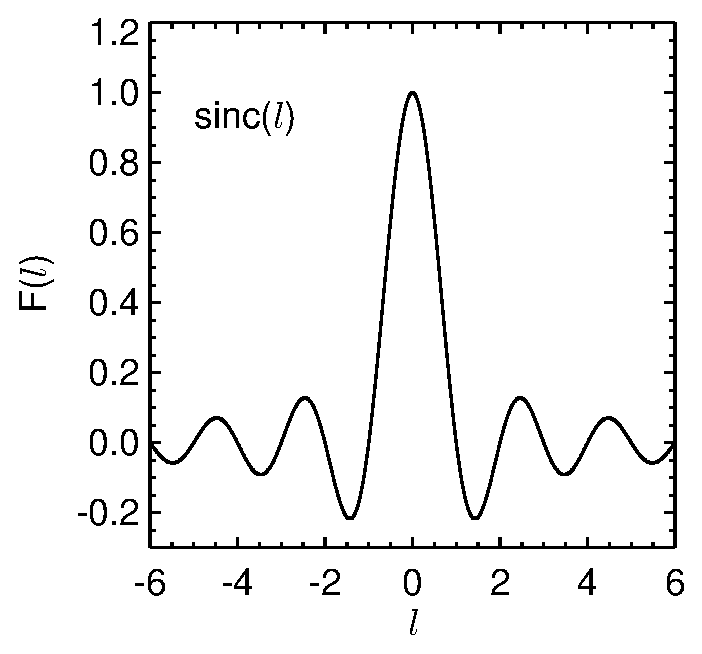
\includegraphics[trim=0pt 0pt 0pt 0pt,clip,width=6.6cm]{/home/eamon/thesis/figures/antenna_beam/fig2b.eps}
          }
\mbox{
          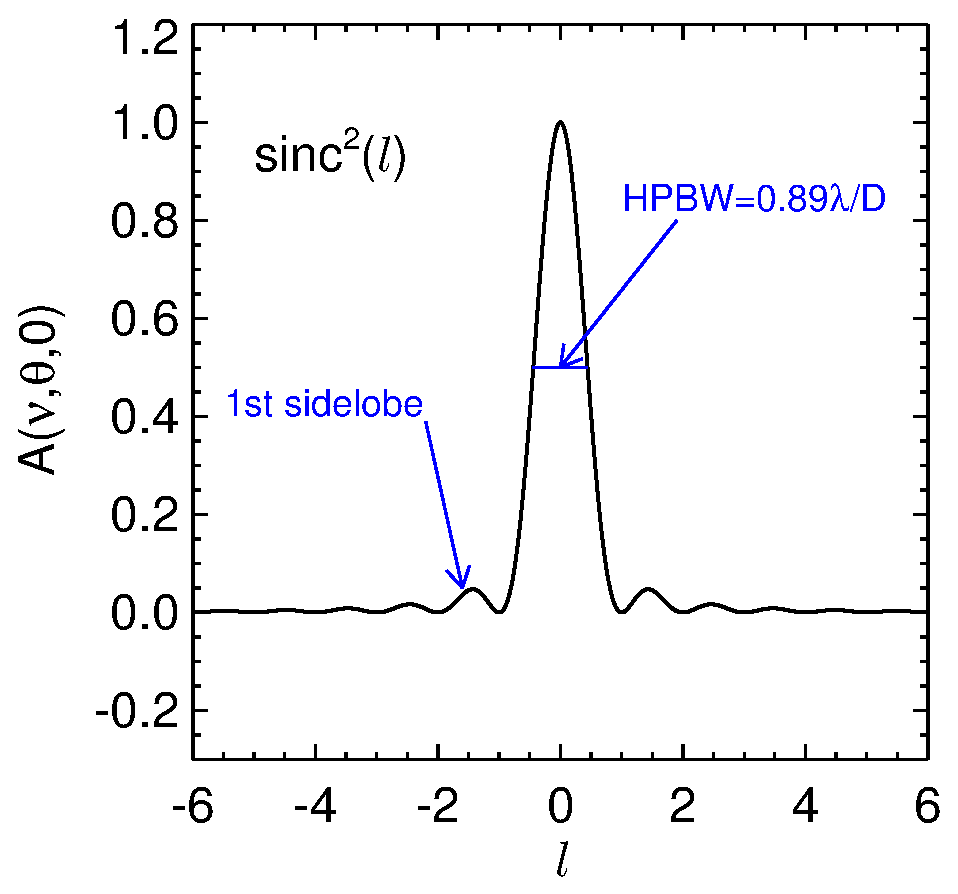
\includegraphics[trim=0pt 0pt 0pt 0pt,clip,width=6.6cm]{/home/eamon/thesis/figures/antenna_beam/fig2c.eps}
          }
\caption[Radiation and power pattern of a uniformly illuminated antenna]{\textit{Top Left:} Uniformly illuminated 1-D aperture $f(u)$. \textit{Top Right:} The Fourier transform of $f(u)$ gives the antenna radiation pattern in the far-field, $F(l)$. \textit{Bottom:} The power pattern of the antenna is given by $\mathcal{A}=|F(l)|^2$.}
\label{fig2.1}
\end{figure}

are the antenna coordinates and $l$ and $m$ are their Fourier counterparts. The form of $f(u,v)$ is determined by the manner in which the antenna feed illuminates the aperture. Therefore Equations \ref{eq:illum1} and \ref{eq:illum2} tell us that the radiation pattern in the far-field of a two-dimensional aperture is the two-dimensional Fourier transform of the aperture field illumination. For a uniformly illuminated 1-D aperture shown in Figure \ref{fig2.1}, the radiation pattern in the far-field is the \textit{sinc} function [i.e., $\mathrm{sinc}(x)=\mathrm{sin}(\pi x)/(\pi x)$]. The radiation pattern in the far-field, $F(l,m)$, of such an antenna is related to the antenna power pattern by $\mathcal{A}=|F(l,m)|^2$. This power pattern is known as the Airy pattern if the antenna is uniformly illuminated and is also shown in Figure \ref{fig2.1}. The central peak of this power pattern is called the main beam while the smaller secondary peaks are called sidelobes. The antenna is maximally sensitive to radiation from the direction of the peak of the beam, but is also slightly sensitive to radiation in the direction of the side lobes. The half-power beamwidth (HPBW) of the main beam $\theta_{\rm{HPBW}}$ is a term commonly used in the literature to describe the field of view of an antenna/interferometer and satisfies 
\begin{equation}
\theta_{\rm{HPBW}} \propto \frac{\lambda}{D}
\end{equation}
where $D$ is the diameter of the antenna. The constant of proportionality varies slightly with the illumination taper and can be shown to be equal to $\sim 0.89$ for a uniformly illuminated 1-D aperture, and $\sim 1.2$ for most single dish radio antennas. When the sky is scanned with a single dish antenna, then this HPBW is the resolution of the resulting map. 
\subsection{Antenna Structural Design}\label{subsec:2.1.2}
The design of the primary antenna element of an interferometric array will depend on the wavelength range to be observed. In general, dipoles are used for wavelengths longer than $\sim$1\,m, while reflector antennas are typically used at shorter wavelengths. The reason why the more simple and less expensive dipoles are not used at all wavelengths is given by Equation \ref{eq:kraus}. For an isotropic antenna, this equation tells us that the effective area is just
\begin{equation}
A_{0} = \frac{\lambda ^2}{4\pi}.
\end{equation}
Therefore, at short wavelengths, a non-directional antenna such as a dipole, will have a small effective collecting area, giving it low sensitivity for reception. Thus, dipoles can be used at long wavelengths as they have sufficient collecting area, but cannot be used at shorter wavelengths as an impractical amount would be needed to produce useful collecting areas. Since the interferometric arrays used in this thesis use reflector antennas, the rest of this section will focus on them.\\
\\
\textit{Choice of Antenna Mount.} Nearly all interferometric arrays consist of antennas which have altitude over azimuth (alt-azimuth) mounts. These antennas lie on a horizontal azimuth track on which the antenna can turn in azimuth, and on a horizontal elevation axle about which the antenna can change in zenith angle. The main advantage of such a design is simplicity and thus lower cost. Gravity always acts on the reflector in the same plan, thus reducing the problem of keeping the reflector profile accurate during the duration of an observation. However, sources close to the zenith cannot usually be observed due to the high rate of azimuth rotation required. In addition, the beam rotates with respect to the source for long duration observations, which can affect the dynamic range of total intensity images of very large sources. The other type of mount occasionally used is the equatorial mount. Its polar axis is aligned parallel to the axis of rotation of the Earth and therefore only needs to rotate around the declination axis to observe a source. Furthermore, its beam doesn't have the beam rotation problem encountered by the alt-azimuth design and can track sources close to the zenith. Its major disadvantage and the reason for its scarce usage is the complexity of its design and resulting increased cost. \\
\\
\textit{Choice of Antenna Optics.} In Figure \ref{fig2.2} we show the main optical systems which can be used to feed a large radio reflector. The prime focus system (e.g., used in the Giant Meter Radio Telescope) has the advantage that it can be used at long wavelengths where the use of secondary focus feeds (i.e., sub-reflectors) become impractical. However, access to and space for the feeds and receivers are limited, and sensitivity can be lost due to spillover noise from the ground. The other designs have the advantage of easier access to the feeds and receivers and less spillover noise from the ground. The off-axis Cassegrain (e.g., used in the Very Large Array) also has the advantage of increased frequency capability as many feeds can be located in a circle around the center of the reflector and a slight rotation of the sub-reflector is all that is required to change observing frequency. The receivers and feeds in the Naysmith geometry (e.g., used in the Combined Array for Research in Millimeter wave Astronomy) are located external to the antenna structure. Finally, the offset Cassegrain (e.g., used in the Green Bank Telescope) has no blockage and will have a circular symmetric beam with low sidelobes.

\begin{figure}[hbt!]
\centering 
          \includegraphics[trim=10pt 40pt 60pt 50pt,clip,width=10.0cm,angle=-90]{/home/eamon/thesis/figures/fig2d.ps}
\caption[Common optical systems used for radio antennas]{Common optical systems used for radio antennas. (\textit{a}) Prime focus, (\textit{b}) Naysmith, (\textit{c}) Off-axis Cassegrain, (\textit{d}) Offset Cassegrain [Figure adapted from \cite{taylor_1999}].}
\label{fig2.2}
\end{figure}

\subsection{Antenna Performance Parameters}\label{subsec:2.1.3}
\textit{Aperture Efficiency.} The geometric collecting area of a parabolic antenna, $A_{\rm{geo}}$ ($=\pi D^2/4$), is related to the effective area (i.e., the collecting area when pointing directly at a source) via the dimensionless quantity, $\eta$ ($\eta < 1$), known as the aperture efficiency where
\begin{equation}
\eta = \frac{A_0}{A_{\rm{geo}}}.
\end{equation}
The aperture efficiency directly impacts on the sensitivity of the interferometric array and can be defined as the product of a number of different efficiency loss factors, 
\begin{equation}
\eta = \eta _{\rm{sf}}\eta _{\rm{bl}}\eta _{\rm{s}}\eta _{\rm{t}}\eta _{\rm{misc}}.
\end{equation}
The surface efficiency, $\eta _{\rm{sf}}$, accounts for the aperture efficiency loss as a result of reflector profile inaccuracies. Such inaccuracies result in the electric field from various parts of the aperture not adding together in phase at the feed, leading to a decrease in power. The aperture blockage efficiency, $\eta _{\rm{bl}}$, accounts for the fact that the sub-reflector (or feed) and its support structure result in a reduction in the incident radiation on the antenna. The feed spillover efficiency, $\eta _{\rm{bl}}$, is best understood if the antenna is considered in transmission rather than in reception mode, and  is defined as the fraction of power radiated by the feed that is intercepted by the reflector for a prime focus system, or by the sub-reflector for a Cassigrain system. The illumination taper efficiency, $\eta _{\rm{t}}$, accounts for the fact that the feed pattern does not illuminate the primary reflector uniformly, but illuminates the outer part of the reflector at a lower level than the inner part. Finally, the miscellaneous efficiency losses such as reflector diffraction and feed position phase errors are accounted for in $\eta _{\rm{misc}}$. As an example, the total aperture efficiency of the VLA antennas can vary between 0.65 and 0.2, at 6 and 0.7 cm, respectively.
\\
\\
\textit{Pointing Accuracy.}
The main lobe of an antenna's power pattern will usually not point exactly in the desired direction, due to gravity deformations, wind pressure deformations, and mechanical inaccuracy. The angular offset, $\Delta \theta$, between the actual and desired pointing direction is called the pointing error. Usually, the desirable pointing error of  an antenna at the highest operational frequency is $\Delta \theta < \theta _{\rm{HPBW}}/20$ \citep{taylor_1999}. With this specification reached, an antenna pointing at a compact source will suffer negligible intensity variations as $\mathcal{A}(\theta _{\rm{HPBW}}/20) > 0.99$. However, this pointing error of only $\theta _{\rm{HPBW}}/20$ will still have a substantial effect on the accuracy of the outer image. For example, a source located at the half power point will suffer a substantial fractional intensity variation of $2\mathcal{A}(\theta _{\rm{HPBW}}/2+\theta _{\rm{HPBW}}/20) \simeq 0.86$. The blind pointing of a VLA antenna is only about 10$^{\prime\prime}$ and can be much worst in daytime, occasionally exceeding 1$^{\prime}$. This means that at Q-band (45 GHz; 0.7 cm), which is the highest observing frequency on the VLA, the pointing error is only at best $\theta _{\rm{HPBW}}/6$, and at worst $>\theta _{\rm{HPBW}}$, meaning that the target may lie outside of the primary beam. To overcome this problem of large antenna pointing errors at high frequencies with the VLA, a technique known as referenced pointing is implemented. This technique will be discussed further in Chapter 3. 

\section{Radio Antenna Receiving System}\label{sec:2.2}

A radiometer (a radio receiver) is a device  used to measure the  timed-averaged power of the noise coming from a radio telescope within a  well-defined radio frequency (RF) range, $\nu _{\rm{RF}}-\Delta \nu _{\rm{RF}}/2 \rightarrow \nu _{\rm{RF}}+\Delta \nu _{\rm{RF}}/2$, where $\Delta \nu _{\rm{RF}}$ is the bandwidth of the receiver and $\Delta \nu _{\rm{RF}}< \nu _{\rm{RF}}$. 
The simplest radiometer carries out the following tasks:
\begin{enumerate}
\item Filters the broadband noise coming from the antenna via a bandpass filter.
\item Multiplies the filtered voltage by itself (i.e., its output voltage is proportional to its input power).
\item Smooths out the rapidly fluctuating output of the detected voltage via a signal averager or integrator.
\item Measures the smoothed voltage.
\end{enumerate}
In practice, radiometers are never as simple as those described above and nearly all practical radiometers are \textit{superheterodyne} receivers which incorporate a number of additional steps to produce an output voltage. The RF front end is the term used to describe all the circuitry between  the feed horn and the lower intermediate frequency (IF) stage. The first task of the front end is to amplify the received signal. The radio signals we want to measure are generally very weak, and therefore need to be initially amplified by many orders of magnitude, so they are above the noise level in succeeding stages. However, the front end electronic components produce random electrical noise which will also get amplified by this large factor. Therefore the role of the pre-amplifier is to amplify the incoming signal from the antenna, while adding as little noise as possible. For this reason, the pre-amplifier is called a low noise amplifier (LNA), and are often cooled to very low temperatures to minimize the amount of noise contributed by the components.

\begin{figure}[hbt!]
\centering 
          \includegraphics[trim=0pt 350pt 0pt 320pt,clip,width=15.0cm]{/home/eamon/thesis/figures/front_end.ps}
\caption[Block diagram of a superheterodyne receiver]{\textit{Left:} Block diagram of a simple superheterodyne receiver. The amplified RF signal is mixed with a signal from a local oscillator to convert the signal to the more manageable intermediate frequency. \textit{Right:} For interferometry, a phase lock loop is used to ensure all antennas are locked to the same frequency. \textit{Image Credit:} Prof. Dale E. Gary (New Jersey Institute of Technology).}
\label{fig2.3}
\end{figure}

The amplified RF signal is then sent through a mixer, which multiplies the RF signal by a sine wave of frequency $\nu _{\rm{LO}}$, which is generated by a local oscillator (LO), as shown in Figure \ref{fig2.3}. The effect of this is that RF signal is changed to a lower frequency which can be more easily handled by the IF amplifier and  improves frequency selectivity. Mathematically, the mixer does the following
\begin{equation}
2\rm{sin}(2\pi \nu _{\rm{LO}}\mathit{t})\times \rm{sin}(2\pi \nu _{\rm{RF}}\mathit{t}) = \rm{cos}[2\pi (\nu _{\rm{LO}}-\nu _{\rm{RF}})\mathit{t}]-\rm{cos}[2\pi (\nu _{\rm{LO}}+\nu _{\rm{RF}})\mathit{t}],
\end{equation}
and produces two additional outputs, one at the input signal frequency minus the local oscillator frequency, and one at the sum of these frequencies. The lower of the two outputs called the intermediate frequency (IF) is taken by passing the mixer output through a filter in the IF amplifier. In interferometry, where the signals from two antennas are correlated, it is crucial that the receivers from both antennas are operating at the same frequency, to control the phase difference between them. This is achieved by using a phase lock system, whose block diagram is laid out in Figure \ref{fig2.3}. In this system another mixer compares the LO to a reference frequency, which is the same for all antennas. Any existing phase error results in an error signal that is sent back to the oscillator, so that its frequency can be adjusted to maintain exact frequency tuning. After this, the IF can finally be sent to the radiometer and recorded.

\section{Fundamentals of Radio Interferometry}\label{sec:3}
The angular resolution, $\Delta \theta$, of a radio antenna is the minimum angular separation which two point sources can have in order to be recognized as separate objects. The \textit{Rayleigh criterion} is the operational defined  angular resolution of a filled circular aperture of diameter, $D$, at the observational wavelength $\lambda$ and is given as
\begin{equation}
\Delta \theta=1.22\frac{\lambda}{D} \ \ \rm{rad}.
\label{eq:rayleigh}
\end{equation}
The Rayleigh criterion states that two objects are resolved when the first null of the diffraction pattern of one object coincides with the maximum of the diffraction pattern of the other. An immediate consequence of Equation \ref{eq:rayleigh} is that at large wavelengths, the angular resolution becomes low unless the diameter of the aperture can be increased substantially. In order to achieve modest angular resolution at radio wavelengths with a single radio antenna, the diameter becomes impractically large. Radio interferometry is a technique used in radio astronomy to overcome this problem of low angular resolution at long wavelengths. For example, the world's largest fully steerable radio telescope is the 100\,m  Robert C. Byrd Green Bank Telescope (GBT), which at 6\,cm can achieve an angular resolution of $2.5^{\prime}$. The VLA on the other hand, in its most extended configuration, can achieve a resolution that is $\sim 400$ times better than that of the GBT, at the same wavelength.



\subsection{Young's Slits}\label{subsec:4}
The basic principles of interferometry can be understood through Young's double-slit experiment. If coherent radiation emitted from a distant point source propagates through two slits, an illumination pattern composed of bright and dark fringes is observed. The phenomenon is a result of the constructive and destructive interference between the secondary waves produced by the slits. The fringe separation is $\lambda /B$, where $B$ is the projected separation of the slits and is called the baseline. The fringe contrast which is historically known as the fringe visibility, $V$, can be written as
\begin{equation}
|V| = \frac{I_{\rm{max}}-I_{\rm{min}}}{I_{\rm{max}} + I_{\rm{min}}}
\end{equation}
where $I_{\rm{max}}$ and $I_{\rm{min}}$ are the maximum and minimum intensity of the fringes, respectively. In other words, the fringe visibility is the fringe amplitude normalized by the sum of the maximum and minimum intensity. 

\begin{figure}[t!]
\centering 
          \includegraphics[trim=0pt 0pt 0pt 0pt,clip,width=12.0cm]{/home/eamon/thesis/figures/youngs.ps}
\caption[Fringe pattern produced by Young's slits]{The resulting fringe pattern produced by Young's slits under various conditions. The source is shown on the left of the slits in each panel, while the separate fringe patterns (colors) along with the added fringe pattern (black) is shown on the right of the slits. (\textit{a}) Point source at infinity, (Visibility = 1). Fringes are separated by an angular distance of $\lambda /B$. (\textit{b}) An increase in source size results in a drop in visibility. (\textit{c}) When the source size is equal to $\lambda /B$, the visibility is zero. (\textit{d}) If the source size remains the same as in (c) and the slit spacing is reduced, then the fringes re-appear. Figure adapted from \cite{jackson_2008}.}
\label{fig2.4}
\end{figure}

In the simple case shown in Figure \ref{fig2.4}a, the angular size of the source is  $\ll \lambda/B$ and the fringe visibility is 1. In interferometry, this equates to the situation in which the source size is smaller than the synthesized beam and only an upper limit of the source size can be obtained (i.e., the source is unresolved). In Figure \ref{fig2.4}b, the angular size of the source is now larger and can be thought of as a sequence of point sources each emitting radiation which is uncorrelated with emission from the others. An angular shift of $\phi$, called phase, in the sources position results in a shift in the corresponding fringe pattern by the same angle the other way. The total interference intensity pattern is then just the sum of these individual patterns and the visibility is reduced. When the extension of the source equals $\lambda/B$, the fringes disappear and give a constant illumination pattern. In this case the fringe visibility is zero and the source is completely resolved as shown in Figure \ref{fig2.4}c. Finally, if the source size is the same as that in Figure \ref{fig2.4}c but the slit separation is reduced, then the fringe separation $\lambda/B$ will again increase as shown in Figure \ref{fig2.4}d. This is because the source now produces much less displacement of the fringe patterns as a fraction of the fringe separation. In interferometry, this result means that extended sources can only be probed with short baselines. 

\begin{figure}[t!]
\centering 
          \includegraphics[trim=0pt 270pt 0pt 250pt,clip,width=12.0cm]{/home/eamon/thesis/figures/visibility.ps}
\caption[Visibilities for various source sizes]{\textit{Left column:} Intensity distribution as a function of sky angle for an extended source (top) and for a more compact source (bottom). \textit{Right column:} The corresponding fringe visibility as a function of slit separation or baseline. Figure adapted from \cite{jackson_2008}.}
\label{fig2.5}
\end{figure}

Visibility and phase are often expressed together as the complex visibility $V=|V|e^{i\phi}$, which completely defines a pattern of interference fringes. Young's double-slit experiment demonstrates a fundamental property of interferometry, namely that the contrast of fringes is a function of the geometry of the source. The results of the experiment are summarized in Figure \ref{fig2.5}. The top row shows that a large source (i.e., one whose intensity distribution extends out to a large angle on the sky) has a fringe visibility pattern which falls off quickly as projected baseline length increases. The bottom row shows that for compact sources, the fringe visibility remains high out to large baselines. In the following sections, we will show that the relationship between the sky brightness distribution $I(\theta)$ and the visibility $V(B)$ is a Fourier transform.

\subsection{The Two-element Interferometer}\label{subsec:5}
Interferometers with $N$ antennas can be treated as $N(N-1)/2$ independent interferometer pairs, so it is worthwhile studying the simplest case of the two-element interferometer. A simplified block diagram of the components of such an interferometer is shown in Figure \ref{fig2.6}. The figure shows two identical antennas separated by a baseline vector, \textbf{b}, pointing towards a distant radio source in a direction indicated by the unit vector, \textbf{s}. The plane waves from the distant radio source reach antenna 1 at a time $\tau _g$ later than they reach antenna 2. $\tau _g$ is called the geometric delay and is given by
\begin{equation}
\tau _{g}=\frac{\textbf{b}.\textbf{s}}{c}=\frac{b\rm{cos}\theta}{c}
\end{equation}
where $c$ is the speed of light. If we assume that the interferometer only responds to a very narrow band centered on frequency $\nu=\omega /2\pi$, then the output voltages of antennas 1 and 2 at time $t$ can be written as 
\begin{equation}
V_1(t)=V\rm{cos}[\omega(\mathit{t}-\tau _g)] \ \ \ \rm{and} \ \ \ \mathit{V_{\rm{2}}(t)=V\rm{cos}(\omega \mathit{t})},
\end{equation}
where $\omega$ is the angular frequency and $V$ is the voltage amplitude. The signals are then passed through a correlator which first multiplies these voltages to give
\begin{equation}
V_1(t) V_2(t)=\frac{V^2}{2}[\rm{cos(2\omega t -\omega \tau _g)+\rm{cos}(\omega \tau _g)}]
\end{equation}
and then averages them over a time interval $\Delta t$ which is long enough such that $\Delta t >> (2\omega)^{-1}$ to give the final power output, $R$:
\begin{equation}
R=\langle V_1(t)V_2(t)\rangle = \frac{V^2}{2}[\rm{cos}(\omega \tau _g)].
\end{equation}
This correlator output is free from uncorrelated noise from the receivers and the atmosphere over the two telescopes, 
and so variations in receiver gain or atmospheric emission are much less of a problem than for a total-power observation with a single dish. 

\begin{figure}[hbt!]
\centering 
          \includegraphics[trim=20pt 160pt 20pt 160pt,clip,width=12.0cm]{/home/eamon/thesis/figures/2_el.ps}
\caption[Simplified schematic diagram of a two-element interferometer]{Simplified schematic diagram of a two-element interferometer. The correlator multiplies and averages the voltage outputs $V_1$ and $V_2$ of the two dishes and yields an output amplitude $V^2/2$ which is proportional to the point-source flux density, $F_{\nu}$. \textit{Image Credit:} National Radio Astronomy Observatory.}
\label{fig2.6}
\end{figure}

As the Earth rotates, $\tau _g$ varies slowly with time and the resultant oscillations in the correlator output voltage represent the motion of the source. These sinusoidal oscillations are called fringes, and the fringe phase is 
\begin{equation}
\phi = \omega \tau _g = \frac{\omega b\rm{cos} \theta}{c}
\end{equation}
which changes with source direction as follows
\begin{equation}
\frac{d\phi}{d\theta}= \frac{\omega b\rm{sin} \theta}{c}=2\pi\left(\frac{b\rm{sin}\theta}{\lambda}\right).
\end{equation}
The fringe phase completes a full period (i.e., $\Delta \phi=2\pi$) when an angular change $\Delta \theta=(\lambda/b\rm{sin}\theta)$ occurs. This tells us that the fringe phase is an extremely sensitive measure of source position if the projected baseline $b\rm{sin}\theta$ is many wavelengths long and is the reason why interferometers can determine the positions of compact radio sources with exquisite accuracy.

\begin{figure}[t!]
\centering 
          \includegraphics[trim=20pt 180pt 20pt 160pt,clip,width=12.0cm]{/home/eamon/thesis/figures/synth_beam.ps}
\caption[Instantaneous point source responses of an interferometer]{The instantaneous point source responses of an interferometer with two, three and four elements is indicated by the thick curves. The individual responses of the three pairs of two-element interferometers of the three-element interferometer and the six pairs of two-element interferometers of the four-element interferometer are plotted as thin curves. The main beam of the four-element interferometer is nearly Gaussian and has a width of $\sim \lambda /B$. This is known as the instantaneous synthesized beam of the interferometer. \textit{Image Credit:} National Radio Astronomy Observatory.}
\label{fig2.7}
\end{figure}

If the antennas in an interferometric array are isotropic, then the  point-source response of the interferometer would be a sinusoid spanning the entire sky, and the interferometer would be only sensitive to one Fourier component of the sky brightness distribution, having angular period $\lambda/b\rm{sin}\theta$. The response of a two-element interferometer $R$ with non-isotropic antennas is this sinusoid, multiplied by the product of the voltage patterns (i.e., defined as $f(u,v)$ in Section \ref{subsec:2.1.1}) of the individual antennas. If the antennas are identical then this product is the power pattern of the individual antennas called the primary beam. The primary beam is usually a Gaussian that is much wider than the fringe period, as $D << b\rm{sin}\theta$ (where $D$ is the antenna diameter). The result is that an interferometer with directive antennas responds to a finite range of angular frequencies centered on $b\rm{sin}\theta /\lambda$. The instantaneous point source response of an interferometer is known as the synthesized beam and is the point source response obtained by averaging the outputs of all antenna pairs. The synthesized beam of an interferometer is an important quantity as it defines the maximum angular resolution of the instrument. The synthesized beams produced by an interferometer with a various number of antennas arranged in 1-D is shown in Figure \ref{fig2.7}. The figure shows that the synthesized beam can be improved by acquiring more Fourier components (i.e., baselines) and rapidly approaches a Gaussian as $N$ increases. However, sidelobes are still significant and a broad negative ``bowl'' exists between the main beam and the first sidelobes, due to the absence of short spacings.

Interferometers have a maximum angular scale that be observed effectively. This scale is often referred to as the \textit{resolving-out scale} or \textit{maximum scale}, and is dependent upon the observing wavelength, $\lambda$, and the minimum projected baseline, $B_{\mathrm{min}}$. Emission will be ``resolved out'' if the observed source contains smoothly varying structures that are larger than this scale. This is an intrinsic property to interferometry and is known as the ``missing flux'' problem. For any array configuration, emission with angular scales of $\sim \lambda/B_{\mathrm{min}}$ or greater is not reproduced in the maps \citep{taylor_1999} and this scale is often used as a guide for the resolving-out scale of a specific array configuration.


\subsection{Complex Visibility}\label{subsec:6}
The interferometer output can be expressed in terms of the radio brightness over the sky, which is sometimes also called specific intensity and has units W m$^{-2}$ Hz$^{-1}$ sr$^{-1}$. If the radio brightness of a spatially extended source in the direction of unit vector \textbf{s} is $I$(\textbf{s}), then the power output of the two-element interferometer with ``cosine'' correlator output near frequency $\nu =\omega/2\pi$ is obtained by treating the extended source as the sum of independent point sources:
\begin{equation}
R_{c}=\int _{\Omega}\mathcal{A}(\textbf{s})I_{\nu}(\textbf{s}) \rm{cos}\left(\frac{2\pi \textbf{b}.\textbf{s}}{\lambda} \right)d\Omega
\end{equation}
where $\mathcal{A}$ is the normalized antenna reception pattern defined in Section \ref{subsec:2.1.1} and we call $\mathcal{A}(\textbf{s})I_{\nu}(\textbf{s})$ the modified brightness distribution. However, the cosine function in the  ``cosine'' correlator output is only sensitive to the even part of the sky brightness distribution, which can be written as the sum of even and odd parts:
\begin{equation}
I(\textbf{s})=I_{\rm{e}}(\textbf{s})+I_{\rm{o}}(\textbf{s}).
\end{equation}
A ``sine'' correlator whose output is odd, is needed to detect the odd part of $I(\textbf{s})$ and this is implemented by inserting a 90$^{\circ}$ phase delay into the signal of one of the antennas to give
\begin{equation}
R_{s}=\int _{\Omega}\mathcal{A}(\textbf{s})I_{\nu}(\textbf{s}) \rm{sin}\left(\frac{2\pi \textbf{b}.\textbf{s}}{\lambda} \right)d\Omega
\end{equation}

It is convenient to write the cosines and sines as complex exponentials using the identity 
\begin{equation}
e^{i\phi} = \rm{cos}(\phi) + \mathit{i}\rm{sin}(\phi)
\end{equation}
and so the combination of ``cosine'' and ``sine'' correlators is called a ``complex'' correlator. The term \textit{visibility} was first introduced by \cite{michelson_1890} to describe the relative amplitudes of the optical fringes that he observed. The visibility is a complex quantity in radio astronomy and has dimensions of spectral power flux density (W m$^{-2}$ Hz$^{-1}$). The complex visibility is the response of a two-element interferometer with a complex correlator to an extended source with brightness distribution $I(\textbf{s})$  and is defined as
\begin{equation}
V\equiv R_{\rm{c}}-iR_{\rm{s}} = Ae^{-i\phi},
\end{equation}
where 
\begin{align}
        A&=\sqrt{R_{c}^2 + R_{s}^2}\\
    \phi &=\mathrm{tan}^{-1}\left(\frac{R_s}{R_c}\right).
\end{align}
This gives the useful relationship between the source brightness, and the response of an interferometer
\begin{equation}
V _{\nu}(\textbf{b}) = \int _{\Omega}\mathcal{A}(\textbf{s})I_{\nu}(\textbf{s})\mathit{e}^{-2\pi \mathit{i} \nu \textbf{b}.\textbf{s}/c}d\Omega ,
\label{eq:visib}
\end{equation}
which under some circumstances, is a 2-D Fourier transform, and allows $I_{\nu}(\textbf{s})$ to be recovered from $V _{\nu}(\textbf{b})$.
\subsection{Coordinate Systems for Imaging}\label{subsec:7}
The projected baseline has coordinates ($u,v,w$) in three dimensions shown in Figure \ref{fig2.8}, where $w$ points in the directions of interest, i.e., towards a direction \textbf{$s_{0}$} that becomes the center of the synthesized image. $u$, $v$ and $w$ are measured in wavelengths (i.e., the components of $\textbf{b}/\lambda$) and have directions towards the East, the North and the phase tracking center, respectively. An arbitrary unit vector \textbf{s} has components ($l,m,n$) called direction cosines, where $n=\rm{cos}\theta=(1-\mathit{l}^2-\mathit{m}^2)^{1/2}$. Using these coordinates, the parameters in Equation \ref{eq:visib} become
\begin{equation}
\begin{split}
\frac{\nu \textbf{b}.\textbf{s}}{c}&=ul+vm+wn, \\
d\Omega &= \frac{dl\,dm}{n}=\frac{dl\,dm}{\sqrt{1-l^2-m^2}}.
\end{split}
\end{equation}
Therefore Equation \ref{eq:visib} can be defined in terms of the coordinate system laid out in Figure \ref{fig2.8} as
\begin{equation}\label{eq:3-d_vis}
\begin{split}
&V_{\nu}(u,v,w)=\\
&\int ^{\infty}_{-\infty}\int ^{\infty}_{-\infty} \mathcal{A}_{\nu}(l,m)I_{\nu}(l,m)\mathit{e}^{-2\pi \mathit{i}[ul+vm+w(\sqrt{1-l^2-m^2})] }\frac{dl\,dm}{\sqrt{1-l^2-m^2}}
\end{split}
\end{equation}
which is not a three-dimensional Fourier transform. This equation becomes a two-dimensional Fourier transform if $w=0$ which is a good approximation for small field imaging, i.e., when $|l|$ and $|m|$ are small. Thus, for a source in the far field observed with a small FOV, and ignoring the response of the primary beam, the complex visibility  is the 2-dimensional Fourier Transform of the sky brightness distribution
\begin{equation}\label{eq:2-d_vis}
V_{\nu}(u,v)=\int ^{\infty}_{-\infty}\int ^{\infty}_{-\infty} I_{\nu}(l,m)\mathit{e}^{-2\pi \mathit{i}(ul+vm)}dl\,dm.
\end{equation}
This Fourier transform relationship is the result of the van Cittert-Zernike theorem \citep{van_cittert_1934}, upon which synthesis imaging is based. Since $I_{\nu}(l,m)$ is real, $V(u,v)$ is Hermitian [i.e.,$V(-u,-v) = V^{*}(u,v)$] and so one measurement of the sky brightness gives two measurements of the complex visibility. Also, $V(u=0,v=0)$ is the integral of $I_{\nu}(l,m)dldm$, which is the total flux. An interferometer cannot measure this value because it cannot take measurements at $(u=0,v=0)$. 

%In this case Equation \ref{eq:3-d_vis} can be inverted to find the modified sky brightness distribution:
%\begin{equation}\label{eq:2dft}
%\mathcal{A}_{\nu}(l,m)I_{\nu}(l,m)=\int ^{\infty}_{-\infty}\int ^{\infty}_{-\infty}V_{\nu}(u,v)\mathit{e}^{2\pi \mathit{i}(ul+vm)}du\,dv.
%\end{equation}
%Therefore Equation \ref{eq:2dft} demonstrates the important Fourier Transform relationship between the sky brightness distribution and the complex visibility (i.e., the interferometer response).

\begin{figure}[t!]
\centering 
          \includegraphics[trim=20pt 150pt 20pt 150pt,clip,width=10.0cm]{/home/eamon/thesis/figures/3d_vis_new.ps}
\caption[Interferometric coordinate system]{The ($u,v,w$) interferometric coordinate system. $l$, $m$, and $n$ are the projections of the unit vector \textbf{s} onto the $u$, $v$, and $w$ axes, respectively. \textit{Image Credit:} \cite{taylor_1999}.}
\label{fig2.8}
\end{figure}

\section{Synthesis Imaging}\label{sec:4}
A synthesis imaging telescope uses the Earth's rotation to vary the projected baseline coverage, thereby increasing the sampling of the $u-v$ plane. In this section we describe how Earth-rotation aperture synthesis is used to convert the complex visibilities outputted from the correlator to a final radio image of the observed sky.
\subsection{Visibility Sampling}\label{subsec:4.1}
An example of how a radio interferometer samples the $u-v$ plane is shown in Figure \ref{fig2.9}. The left panel of this figure shows the overhead view of the VLA in its most extended configuration, while the other two panels show the corresponding $u-v$ coverage for different periods of time. We define $u$ and $v$ as the east-west and north-south components of the projected baseline in wavelengths, respectively. As the Earth rotates, the projected baseline of every two-element pair in the array changes, thus sampling a different part of the $u-v$ plane. The middle panel shows that the total $u-v$ coverage of the VLA for a very short duration track (i.e., a \textit{snapshot}) results in a ``snowflake'' like pattern, with more dense coverage in the direction of the arms of the array due to the larger number of baselines. Most radio interferometers have their own unique array configuration layout and thus produce a different snapshot $u-v$ coverage to that shown in Figure \ref{fig2.9}. Over many hours, the $u-v$ points trace out portions of ellipses and eventually after a full Earth rotation the points can trace out full ellipses as shown in the right panel of Figure \ref{fig2.9}. 

\begin{figure}[hbt!]
\centering 
          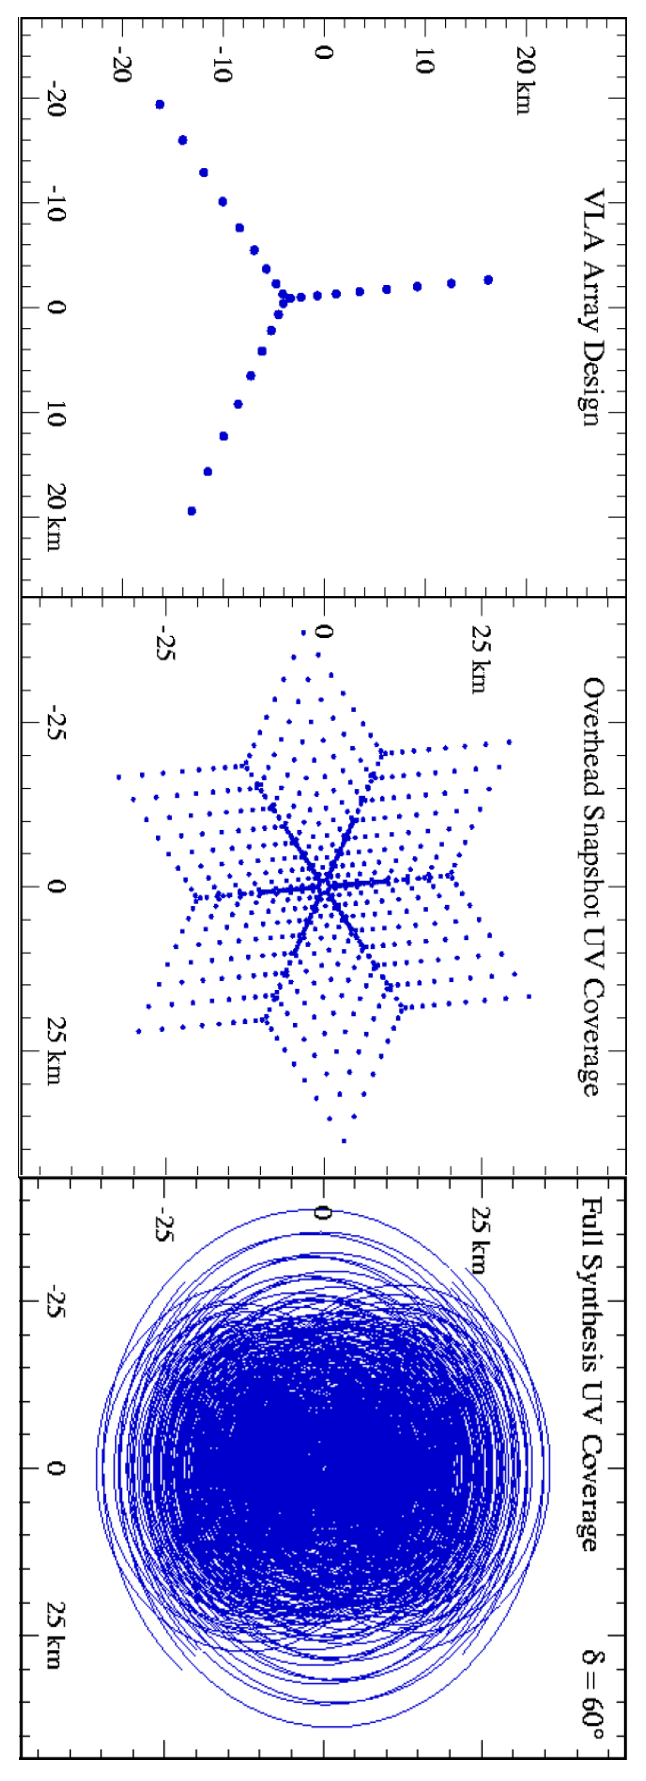
\includegraphics[angle=90,trim=0pt 0pt 0pt 0pt,clip,width=13.5cm, height=5.0cm]{/home/eamon/thesis/figures/uv_coverage.eps}
\caption[VLA antenna layout and two examples of $u-v$ coverage]{\textit{Left:} The VLA in A-configuration is an example of an ``Y'' shaped array design. \textit{Middle:} The corresponding overhead snapshot $u-v$ coverage results in ``snowflake'' pattern. \textit{Right:} The corresponding $u-v$ coverage after a 12 hour track of a source at a declination of 60$^{\circ}$. Note the more intense $u-v$ coverage in the direction of the three straight arms of the VLA for a snapshot track compared to the more uniform coverage over a longer duration track. \textit{Image Credit:} National Radio Astronomy Observatory.}
\label{fig2.9}
\end{figure}

\subsection{Imaging (Making a Dirty Map)}\label{subsec:4.2}
For every sky brightness distribution $I(l,m)$ there exists a continuous complex visibility function, $V(u,v)$, which is its Fourier Transform. An array of antennas will only ever measure a certain set of values of this visibility function where the measured set is called the sampling function $S(u,v)$. This function is zero where no data have been taken. The actual data provided by the array is known as the sampled visibility function, $S(u,v)V(u,v)$. If we take the inverse Fourier transform of this function we get what is known as the \textit{dirty image}:

\begin{equation}\label{eq:dirtyim}
I_{\nu}^{D}(l,m)=\int ^{\infty}_{-\infty}\int ^{\infty}_{-\infty}S(u,v)V_{\nu}(u,v)\mathit{e}^{2\pi \mathit{i}(ul+vm)}du\,dv.
\end{equation}
where we have used $I_{\nu}(l,m)$ to denote the modified sky brightness $\mathcal{A}(l,m)I_{\nu}(l,m)$, as the correction for primary beam can be made at the final stage of data processing. Using the convolution theorem, the relationship between the dirty image and the desired intensity distribution $I_{\nu}(l,m)$ is
\begin{equation}\label{eq:dirty_image}
I_{\nu}^{D}(l,m)=I_{\nu}(l,m)*B(l,m)
\end{equation}
where the asterisk implies convolution and
\begin{equation}\label{beam_samp}
B(l,m) = \int ^{\infty}_{-\infty}\int ^{\infty}_{-\infty}S(u,v)\mathit{e}^{2\pi \mathit{i}(ul+vm)}du\,dv
\end{equation}
is the \textit{point spread function} (PSF), or \textit{synthesized beam}, or \textit{dirty beam} (i.e., the inverse Fourier Transform of the sampling function $S$). Equation \ref{eq:dirty_image} says that the dirty image, $I^{D}_{\nu}$, is the true intensity distribution $I_{\nu}$, convolved with the synthesized beam, $B$.

In Figure \ref{fig2.10} we graphically summarize what has been said above. The panels in the upper row show the sky plane representations of the true image, the point spread function, and the dirty image, while the panels in the lower row show the corresponding $u-v$ plane representations of the true visibility, the sampling function, and the sampled visibility. In other words, Equation \ref{eq:2-d_vis} is summarized graphically by the relationship between panels (a) and (d),  Equation \ref{beam_samp} by (b) and (e), and Equations \ref{eq:dirtyim} and \ref{eq:dirty_image} by (c) and (f).

\begin{figure}[t!]
\centering 
          \includegraphics[trim=0pt 260pt 0pt 260pt,clip,width=14.0cm]{/home/eamon/thesis/figures/ft_ift.ps}
\caption[The Fourier transform pairs in synthesis imaging]{The Fourier transform pairs in synthesis imaging. (a) and (d): The true sky brightness and the visibility. (b) and (e): The dirty beam and the sampling function. (c) and (f): The dirty image and the sampled visibility. \textit{Image Credit:} Prof. Dale E. Gary (New Jersey Institute of Technology).}
\label{fig2.10}
\end{figure}

Before the dirty image is computed, a weighting system is often applied to the visibilities to control the PSF. The two most common types of weighting system used are:
\begin{equation}
D_{k}=1,	\ \ \ \ \ \ \ \rm{natural \ weighting}
\end{equation}
\begin{equation}
D_{k}=\frac{1}{N_{s}(k)}, \ \ \ \ \ \rm{uniform \ weighting}
\end{equation}
where $D_{k}$ is the weight to be applied to cell $k$, and ${N_{s}(k)}$ is the number of data samples falling into cell $k$ of characteristic width $s$. Natural weighting treats all points alike, and gives the best S/N for detecting weak sources. However, it produces a beam with a broad low-level plateau which is undesirable when imaging sources with both large and small scale structure. Uniform weighting produces fewer artifacts in the final map, while keeping the full resolution of the array but gives lower S/N than natural weighting.

The ``direct Fourier transform'' method can then be used to solve for the dirty image in Equation \ref{eq:dirtyim}. However, if this method is evaluated at every point on a $N\times N$ grid, then the number of multiplications required goes as $N^{4}$. The fast Fourier transform (FFT) algorithm can also be used to solve Equation \ref{eq:dirtyim} but requires interpolating the data onto a regular grid (i.e., a process known as \textit{gridding}). This method is widely used for large data volumes as it requires only a few times $N^{2}\rm{log}_{2}\mathcal{N}$ operations - not $\mathcal{O}(N^4)$, and the total time taken for gridding and FFT is usually a lot less than it would take using the direct Fourier transform method.

\subsection{Deconvolution (Making a CLEAN map)}\label{subsec:4.3}
In reality, Equation \ref{eq:dirty_image} contains an additional noise, $n$, term so that
\begin{equation}\label{eq:dirty_noise}
I^{D}=I*B + n.
\end{equation}
The goal of image reconstruction is to recover $I$ from this equation. Mathematically, one could solve Equation \ref{eq:dirty_noise} by first taking the Fourier transform of both sides, then use the convolution theorem to allow division by the Fourier transform of $B$, and finally recover $I$ by taking the inverse Fourier transform of both sides to get
\begin{equation}\label{eq:solution}
I=\mathrm{IFT}\left(\frac{\mathrm{FT}(I^D)-\mathrm{FT}(n)}{\mathrm{FT}(B)}\right),
\end{equation}
where FT and IFT represent the Fourier transform and the inverse Fourier transform, respectively. However, there are two main problems associated with solving Equation \ref{eq:dirty_noise} by this method. First, the presence of the noise term means that the division by $\mathrm{FT}(B)$ amplifies the noise and introduces high frequency artifacts into $I$ \citep{taylor_1999}. Also, Equation \ref{eq:solution} is not unique, because the unmeasured points in the $u-v$ plane could have \textit{any} value without violating the data constraints. The ``principle solution'' is the one in which all missing $u-v$ measurements are set to zero and gives the dirty image discussed in the previous section. The dirty image is usually not a satisfactory representation of the sky as one would expect a more continuous distribution of visibilities than that provided by the array. The goal of the deconvolution process is to find a method that determines more reasonable values for the unmeasured $u-v$ data. A priori information is the key to choosing \textit{reasonable} values. For example, we know that the Stokes parameter $I$ must be positive and that radio sources generally do not have sidelobe patterns.
 
The CLEAN algorithm \citep{hogbom_1974, schwarz_1978, cornwell_1999} is the most widely used technique in radio interferometry to deconvolve the true sky intensity from the dirty beam. It assumes that the radio source can be represented by a number of point sources in an otherwise empty field and a simple iterative process is used to find the strengths and positions of these point sources. The final CLEAN image (i.e., the deconvolved image) is the sum of these point sources convolved with a CLEAN beam, which is usually an elliptical Gaussian of the same size and shape as the inner part of the dirty beam. The CLEAN algorithm obeys the following steps:
\begin{enumerate}
\item Find the strength and position of the brightest point in the dirty image. It may also be desirable to search for peaks in specified areas of the image, called CLEAN windows or regions.
\item At this position in the dirty image, subtract the dirty beam multiplied by the peak strength and a damping factor $g$ ($g \le 1$, usually called the loop gain).
\item Record the position and the subtracted flux in a model.
\item Iterate between (1), (2), and (3) until the peak is below some user specified level. The remainder of the dirty image is now  termed the residuals.
\item Convolve the accumulated point source model with an idealized CLEAN beam (usually an elliptical gaussian of the same size and shape as the central lobe of the dirty beam).
\item Add the residuals to the image in (5) to create the final CLEAN image.
\end{enumerate}
A problem with CLEAN is that the final CLEANed image is somewhat dependent upon the various control parameters such as CLEAN boxes, the loop gain and the number of CLEAN subtractions. For example, using too high a gain tends to make extended, weak emission undetectable and noisy. This problem is unavoidable, and input values must be chosen on a case by case basis, depending on the source and data quality.

Another deconvolution algorithm used in radio synthesis imaging, albeit less often, is the Maximum Entropy Method (MEM) which operates by minimizing a smoothness function (``entropy'') in an image. To conclude this section, we briefly discuss the practical differences between CLEAN and MEM:
\begin{enumerate}
\item CLEAN is nearly always faster than MEM, unless the image contains more than 1 million pixels.
\item MEM images are nearly always smoother than CLEAN images. This is because for CLEAN, what happens at one pixel is not coupled to what happens to its neighbours, while MEM couples pixels together by minimizing the spread in pixel values.
\item CLEAN sometimes makes extended emission look blotchy and may introduce artificial stripes into the image while MEM copes very poorly with point sources in extended emission. (Multi-scale CLEAN which is discussed in Chaper \ref{chap:3} is now becoming a popular choice in the radio community as an alternative deconvolution algorithm for images containing extended emission.)
% Multiscale CLEAN: http://iopscience.iop.org/1538-3881/136/6/2897/fulltext/
\item For MEM, it is necessary to know the noise level quite well and it also helps to know the total flux density of the image. Knowledge of these are not required for CLEAN.
\end{enumerate}


%%!TEX root = ../thesis.tex
%Adding the above line, with the name of your base .tex file (in this case "thesis.tex") will allow you to compile the whole thesis even when working inside one of the chapter tex files

\chapter{Targets, Instrumentation, and Observations} \label{chap:3}

\section{Betelgeuse}\label{sec:3.1}
decin proposal, paper intro, CO

\begin{table}
\begin{center}
\caption[Physical Properties of $\alpha$ Ori.]
{Physical Properties of $\alpha$ Ori.}
\begin{tabular}{lcc}
\hline
\hline
\rule{0pt}{2.5ex}Property & $\alpha$ Ori & Reference \\
\hline
\rule{0pt}{2.5ex}HD Number & 124897 & \\
Spectral Type & K2 III &\\ 
ra (ICRS: ep=J2000)&14$^{\rm{h}}$15$^{\rm{m}}$39.672$^{\rm{s}}$&\\
dec (ICRS: ep=J2000) & +19 10 56.673 & \\
pm-ra (mas yr$^{-1}$)& $-1093.39 \pm 0.44$ & \\
pm-dec (mas yr$^{-1}$)& $-2000.06 \pm 0.39$ & \\
$\pi$ (mas)& $88.83\pm 0.54$ &\\
Distance (pc)& 11.3$\pm$0.1 & \\
$M$ ($M_{\odot}$) & 0.8$\pm$0.2 & \\
$\theta _{\rm{UD}}$ (mas)& 21.0$\pm$0.2 & \\
$\theta _{\rm{LD}}$ (mas)& 21.0$\pm$0.2 & \\
L ($L_{\odot}$)& &  \\
$R$ ($R_{\odot}$)& 25.4$\pm$0.3 & \\
Log $g$ & &  \\
$T_{\rm{eff}}$ (K) & 4294$\pm$30 & \\
$v_{\rm{rad}}$ (km s$^{-1}$) & $+5.19 \pm 0.04$ & \\
$v_{\rm{esc}}$ (km s$^{-1}$) &110 & \\
$v_{\rm{\infty}}$ (km s$^{-1}$)& $\sim$40 & \\
$T_{\rm{wind}}$ (K)& $\sim$10,000 & \\
$\dot{M}$ ($M_{\odot}$ yr$^{-1}$)& \\
$H$ ($H_{\odot}$)& & \\
 Fe/H& -0.5$\pm$0.2 &\\
\hline
\rule{0pt}{2.5ex}
\end{tabular}
\label{tab:3.1}
\end{center}
\end{table}

\section{CARMA}\label{sec:3.2}


\section{CARMA Observations of Betelgeuse}\label{sec:3.3}
3 configurations, max and min resolutions, variability of phase cals, flux cals
\begin{landscape}
\begin{table}
\begin{center}
\caption[CARMA Observations of $\alpha$ Ori.]
{CARMA Observations of $\alpha$ Ori between June 2007 and November 2009.}
\begin{tabular}{lccccc}
\hline
\hline
\rule{0pt}{2.5ex}Date & Configuration & Time on Source & Flux		& Phase 	& Image Cube \\
	 & 				 &  (hr)		  & Calibrator	& Calibrator& Dynamic Range \\
\hline
\rule{0pt}{2.5ex}2007 Jun 18 	& D & 0.9 & 0530+135	& 0530+135, 0532+075 	&  22.8 \\
2007 Jun 21 	& D & 3.0 & 0530+135	& 0530+135, 0532+075 	&  22.7 \\
2007 Jun 24 	& D & 2.1 & 0530+135	& 0530+135, 0532+075 	&  26.1 \\
2007 Jun 25 	& D & 2.4 & 0530+135	& 0530+135, 0532+075 	&  30.2 \\
2009 Jul 07	& E & 3.2 & 3C120 		& 3C120, 0532+075	& 30.1 \\
2009 Nov 05	& C & 1.2 & 3C120 		& 3C120, 0532+075 	& 17.3 \\
2009 Nov 09 	& C & 3.0 & 3C120 		& 3C120, 0532+075 	& 27.2 \\
2009 Nov 15	& C & 1.0 & 3C120 		& 3C120, 0532+075 	& 17.8 \\
2009 Nov 16	& C & 3.2 & 3C120 		& 3C120, 0532+075 	& 32.0  \\
All		& C & 8.4	&  $\dots$	& 	$\dots$	& 43.8 \\
All 		& D & 8.4 &  $\dots$	&  	$\dots$	& 31.9 \\
All 		& Multi-configuration & 20.0 & $\dots$& $\dots$ 	& 52.3 \\
\hline
%\tablenotetext{a}{Central frequency of selected bandpass.}
%\tablenotetext{b}{Number of available antennae remaining after flagging.}
\end{tabular}
\label{tab:1}
\end{center}
\end{table}
\end{landscape}

\section{Arcturus and Aldebaran}\label{sec:3.4}
wood paper, paper into, ken proposal re arcturus
\begin{table}
\begin{center}
\caption[Physical Properties of $\alpha$ Boo and $\alpha$ Tau.]
{Physical Properties of $\alpha$ Boo and $\alpha$ Tau.}
\begin{tabular}{lccc}
\hline
\hline
\rule{0pt}{2.5ex}Property & $\alpha$ Boo & $\alpha$ Tau & Reference\\
\hline
\rule{0pt}{2.5ex}HD Number & 124897 & 29139 & $\ldots$\\
Spectral Type & K2 III & K5 III& 1, 2\\ 
ra (ICRS: ep=J2000)&14$^{\rm{h}}$15$^{\rm{m}}$39.672$^{\rm{s}}$&04$^{\rm{h}}$35$^{\rm{m}}$55.239$^{\rm{s}}$&3\\
dec (ICRS: ep=J2000) & +19 10 56.673 & +16 30 33.489 & 3 \\
pm-ra (mas yr$^{-1}$)& $-1093.39 \pm 0.44$ & $63.45\pm 0.84$  & 3 \\
pm-dec (mas yr$^{-1}$)& $-2000.06 \pm 0.39$ & $-188.94\pm 0.65$ & 3 \\
$\pi$ (mas)& $88.83\pm 0.54$ & $48.94\pm 0.77$& 3\\
Distance (pc)& 11.3$\pm$0.1 & 20.4$\pm$0.3& 3\\
$M$ ($M_{\odot}$) & 0.8$\pm$0.2 & 1.3$\pm$0.3& 6, 4 \\
$\theta _{\rm{UD}}$ (mas)& 21.0$\pm$0.2 & 20.2$\pm$0.3& 5 \\
$\theta _{\rm{LD}}$ (mas)& 21.0$\pm$0.2 & 20.2$\pm$0.3& 5 \\
L ($L_{\odot}$)& & & \\
$R$ ($R_{\odot}$)& 25.4$\pm$0.3 & 44.4$\pm$1.0 & $\ldots$ \\
Log $g$ & & & \\
$T_{\rm{eff}}$ (K) & 4294$\pm$30 & 3970$\pm$49& 5 \\
$v_{\rm{rad}}$ (km s$^{-1}$) & $+5.19 \pm 0.04$ & $+54.11\pm 0.04$ & 9\\
$v_{\rm{esc}}$ (km s$^{-1}$) &110 & 106& $\ldots$\\
$v_{\rm{\infty}}$ (km s$^{-1}$)& $\sim$40 & $\sim$30& 7, 8\\
$T_{\rm{wind}}$ (K)& $\sim$10,000 & $<$10,000 & 7, 8\\
$\dot{M}$ ($M_{\odot}$ yr$^{-1}$)& $2\times 10^{-10}$& $1.6\times 10^{-11}$& 7, 8\\
$H$ ($H_{\odot}$)& & & $\ldots$\\
Fe/H& -0.5$\pm$0.2 & 0.00$\pm$0.2 & 10\\
\hline
\end{tabular}
\label{tab:1}
\begin{minipage}{13.0cm}
References.-(1);(2)\cite{gray_2006}; (3)\cite{van_leeuwen_2007}; (5)\cite{di_benedetto_1993};
(6)\cite{kallinger_2010}; (7)\cite{drake_1985}; (8)\cite{robinson_1998}
(9)\cite{massarotti_2008}; (10)\cite{decin_2003}
\end{minipage}
\end{center}
\end{table}

\section{The Karl G. Jansky Very Large Array}\label{sec:3.5}
The Karl G. Jansky Very Large Array (VLA) is an aperture synthesis radio telescope located on the Plains of San Agustin, New Mexico, USA and is capable of producing radio images with a resolution comparable to that of optical telescopes. It is the product of a program to modernize the electronics of the `old' Very Large Array which had been in operation since the late 1970's. A comparison of the performance parameters of the VLA with those of the `old' Very Large Array is shown in Table \ref{tab:3.1}. The three major new observational abilities of the VLA are:
\begin{enumerate}
\item Complete frequency coverage between 1 and 50 GHz.
\item An increase in continuum sensitivity by an order of magnitude at some frequencies, by increasing the bandwidth to 8 GHz per polarization.
\item Process the large bandwidth with a minimum of 16,384 spectral channels per baseline.
\end{enumerate}

The structural design of the VLA has not changed during its recent upgrade. As before it consists of 27 fully steerable alt-azimuth antennas arranged along the arms of an upside-down `Y'.  The array is reconfigurable and can vary its resolution by over a factor of $\sim 50$ through movement of its component antennas along twin railroad tracks. Four standard configurations of antennas along the arms of the array are possible whose scales vary by the ratios 1 : 3.28 : 10.8 : 35.5 from smallest to largest. These are called D, C, B, and A configurations, with A having the longest baselines ($\sim 36$ km) giving the best angular resolution, but lacking short baselines needed for imaging extended structure. In each configuration, the distance of each antenna from the center of the `Y' is equal to $m^{\rm{ln}2}$ where $m$ is the antenna location number, counting outwards from the center of each arm. With this design, the $m$'th station in any configuration coincides with the 2$m$'th station in the next smaller configuration. This means that only 72 stations are needed to handle all four configurations. Additionally, there are 3 `hybrid' configurations called DnC, CnB, and BnA, which are well suited for sources with either very low or very high declinations. In these configurations, the North arm antennas are deployed in the next larger configuration than the SE and SW arm antennas resulting in a more circular dirty beam for these sources.

\begin{table}
\begin{center}
\caption[Improved Performance Parameters of the VLA.]
{Improved Performance Parameters of the VLA.}
\begin{tabular}{lccc}
\hline
\hline
\rule{0pt}{2.5ex}Parameter & `old' VLA & VLA & Improvement Factor \\
\hline
\rule{0pt}{2.5ex}Continuum sensitivity (1$\sigma$, 9 hr) & 10 $\mu$Jy & 1 $\mu$Jy& 10\\
Bandwidth per polarization & 0.1 GHz & 8 GHz & 80\\ 
Coarsest frequency resolution & 50 MHz & 2 MHz & 25\\ 
Finest frequency resolution & 381 Hz & 0.12 Hz & 3180\\ 
Channels at max. bandwidth & 16 & 16,384 & 1024\\ 
Maximum number of channels & 512 & 4,194,304 & 8192\\ 
\hline
\rule{0pt}{2.5ex}
\end{tabular}
\label{tab:3.1}
\end{center}
\end{table}

Each antenna is 25 m in diameter giving the array a total collecting area equivalent to a single dish of 130 m in diameter. Each antenna has an off-axis Cassegrain design with a rotatable sub-reflector on a movable mount at the prime focus of the main reflector supported by four feed legs. All feeds are located on a feed ring at the Cassegrain focus and the observing feed is changed by rotating the asymmetric sub-reflector about the main reflector axis so that the secondary focal point moves to the desired feed. The standard observing mode for all feeds is circular polarization. Directly underneath the main reflector is a temperature controlled vortex room, in which lies the front ends and their the cryogenic cooling systems, portions of the local oscillator (LO) and intermediate frequency (IF) equipment. Waveguides from the feeds directly connect to the front end. IF signals from each antenna are sent by cable to a shielded room where the sampler and delay and multiplier racks are located. Once the signals have been cross-correlated they are time averaged into visibility measurements.
\section{VLA Observation Preparation}\label{sec:3.6}

\section{VLA Observations of Arcturus and Aldebaran}\label{sec:3.7}

settings, calibrators, images of flux and phase

\begin{landscape}
\begin{table}
\begin{center}
\caption[VLA Observations of $\alpha$ Boo and $\alpha$ Tau.]
{VLA Observations of $\alpha$ Boo and $\alpha$ Tau obtained in February 2011 and July 2012.}
\begin{tabular}{lccccccccc}
\hline
\hline
\rule{0pt}{2.5ex}Star & Date & Band & $\nu$	& $\lambda$& Time on& Restoring Beam			& Bandwidth & Number of&Phase\\
	 & 		&  & (GHz)		& (cm)		& Star (hr)		  & ($\arcsec \times \arcsec$)& (GHz)		& Antennas&Calibrator\\
\hline
\rule{0pt}{2.5ex} $\alpha$ Boo 	& 2011 Feb 22 & Q	& 43.3 & 0.7		& 0.3 	&0.19 $\times$ 0.15& 0.256	&22& J1357+1919  \\
				& 2011 Feb 22 & Ka	& 33.6 & 0.9		& 0.2 	&0.25 $\times$ 0.20& 0.256 	&23&J1357+1919  \\
				& 2011 Feb 22 & K	& 22.5 & 1.3		& 0.4	&0.35 $\times$ 0.28& 0.256 	&24&J1357+1919  \\
				& 2011 Feb 11 & X	& 8.5  & 3.5		& 0.3 	&1.14 $\times$ 0.70& 0.256 	&18&J1415+1320  \\
				& 2011 Feb 11 & C	& 5.0  & 6.0 		& 0.5	&2.02 $\times$ 1.30& 0.256 	&21& J1415+1320 \\
				& 2011 Feb 13 & S	& 3.1  & 9.5 		& 1.8 	&2.57 $\times$ 2.08& 0.256 	&12& J1415+1320 \\
				& 2012 Jul 19 & S	& 3.0  & 10.0 		& 0.7 	&2.82 $\times$ 2.30& 2.0		&23& J1415+1320 \\
				& 2012 Jul 20 & L	& 1.5  & 20.0		& 1.6 	&4.46 $\times$ 3.94& 1.0		&23& J1415+1320 \\
\hline
\rule{0pt}{2.5ex}  $\alpha$ Tau	& 2011 Feb 11 & Q	& 43.3 & 0.7 		& 0.3 	&0.18 $\times$ 0.16& 0.256 	&22&  J0431+1731\\
				& 2011 Feb 11 & Ka	& 33.6 & 0.9 		& 0.2 	&0.22 $\times$ 0.20& 0.256 	&19&  J0449+1121\\
				& 2011 Feb 11 & K	& 22.5 & 1.3 		& 0.4 	&0.35 $\times$ 0.31& 0.256 	&21&  J0449+1121\\
				& 2011 Feb 13 & X	&  8.5 & 3.5 		& 0.5	&0.85 $\times$ 0.78& 0.256 	&25&  J0449+1121\\
				& 2011 Feb 13 & C	&  5.0 & 6.0 		& 1.2	&1.48 $\times$ 1.32& 0.256 	&21&  J0449+1121\\
				& 2011 Feb 12 & S	&  3.1 & 9.5 		& 1.8 	&2.74 $\times$ 2.02& 0.256 	&11&  J0431+2037\\ 
\hline
%\tablenotetext{a}{Central frequency of selected bandpass.}
%\tablenotetext{b}{Number of available antennae remaining after flagging.}
\end{tabular}
\label{tab:1}
\end{center}
\end{table}
\end{landscape}


%!TEX root = ../thesis.tex
%Adding the above line, with the name of your base .tex file (in this case "thesis.tex") will allow you to compile the whole thesis even when working inside one of the chapter tex files

\chapter{Radio Interferometric Data Analysis} \label{chap:4}

The complex visibilities outputted from the correlator of a radio interferometer are far from ideal and many additional steps of processing are required before they can be of scientific use. The imperfection of the synthesis radio telescopes (e.g., surface accuracy, receiver noise, gain stability, etc.), the adjustments to the signal (e.g., filter bandpass, etc.), hardware or software failures, poor atmospheric conditions, and the presence of RFI are some of the many sources of visibility corruption that must be accounted for before they can be Fourier transformed to get the sky brightness distribution. The chapter describes the three main steps involved in reducing any standard radio interferometric data set, namely: data examination and flagging, data calibration, and imaging. In each step we give relevant examples of the data reduction techniques used in \cite{ogorman_2012} and \cite{ogorman_2013}. A general work flow chart is given in Figure \ref{fig:4.1} which highlights the standard procedure required to go from raw visibilities to image analysis and summarizes what will be discussed in this chapter.\\
\\
\begin{figure}[hbt!]
\centering 
          \includegraphics[trim=20pt 220pt 0pt 200pt,clip,scale=0.74]{/home/eamon/thesis/thesis_template/4/cash_flow.ps}
\caption[Radio interferometry work flow chart]{Work flow chart highlighting the general procedure required to go from the raw visibilities outputted by the correlator to a final radio image that can be used for scientific analysis. (Image adapted from the CASA cookbook, NRAO)}
\label{fig:4.1}
\end{figure}

\section{Data Examination and Flagging}\label{sec:4.1}
The Common Astronomy Software Application \citep[CASA;][]{mcmullin_2007} package was used to flag, calibrate, and image the main data sets used in this thesis. CASA is operated through a Python interface and uses a suite of astronomical data reduction tools which have been developed to meet the processing requirements of the large  data sets from the Karl G. Jansky VLA and ALMA. It can also be used to process data from practically all other modern radio synthesis arrays. For synthesis data to be processed in CASA, it must be in a ``measurement set'' format. VLA data is easily transferable into this format using the \textit{importevla} task within CASA. CARMA data files however come in \textit{Miriad} format and need to be first converted into Flexible Image Transport System (FITS) format within the Miriad \citep{sault_1995} data reduction package. During this process the raw data are smoothed by a Hanning filter (combining adjacent frequency channels with weights 0.25, 0.5, and 0.25) to dampen ringing in the bandpass. Once in FITS format, the data can then be imported into CASA using the \textit{importuvfits} task.

Once the data has successfully been imported into CASA the \textit{listobs} task can be used to get a summary of the data set, allowing the user to make sure the observing track contains the requested sources observed at the correct times. At this point it is also a good idea to check any observing logs which are created on site during the observation by the array operators. These logs contain important information about specific tracks such as non-operational antennas or unavailable receivers, and such data will either need to be treated appropriately during calibration or flagged at this stage. The \textit{plotms} task, which is a GUI-style plotter, can then be used to obtain X-Y plots of the visibility data. A good visual overview of the observation track is obtained by plotting all the source visibility amplitudes as a function of time. Averaging the data over channels or baselines often alerts the user to obvious bad data, which can be manually flagged through the \textit{plotms} interface or through the \textit{flagdata} task. An example of such a plot is shown in Figure \ref{fig:4.2} where the visibility amplitudes of three sources in a 1.3\,cm VLA observing track for Aldebaran are displayed against time. The relatively weak target is shown between interleaving scans of the stronger phase calibrator, while the flux calibrator is the scan at the end of the observing track and is the strongest source in this observation. The data can be averaged over channels or baselines to speed up the plotting process. Some relatively low visibility amplitudes can clearly be seen for all scans of the phase calibrator, which can be traced to a single poor performing antenna.

\begin{figure}[hbt!]
\centering 
\includegraphics[trim=20pt 240pt 0pt 230pt,clip,scale=0.75]{/home/eamon/thesis/thesis_template/4/c_overview.ps}  
\caption[Data examination of a VLA data set]{Data examination of a 6\,cm VLA data set for Aldebaran. A good visual overview of the observation track is obtained by plotting all the source visibility amplitudes as a function of time. Averaging the data over channels or baselines sometimes allow rogue data to stand out. Here the black, orange, and green data points represent the phase calibrator, the science source, and the flux calibrator, respectively. The left most black data points are part of the dummy scan which was subsequently flagged. The low data points of the phase calibrator are data which needs further investigation. The absence of data at certain times represent observations at 3\,cm.}
\label{fig:4.2}
\end{figure}

Another important way to represent the data at this stage of the flagging process is to plot the visibility amplitude of each of the sources as a function of $u-v$ distance or baseline length (i.e., $\sqrt{u^2 + v^2}$). The amplitude distribution should be relatively constant as a function of $u-v$ distance for the phase calibrator (i.e., a point source) and will fall off with increasing baseline length if the flux calibrator is resolved. Plotting the data in this format often results in extreme points at certain baselines which can then often be traced back to poorly behaving antennas or corrupt baselines. There is also some flagging which can be carried out based in part on a priori information. Antennas in very compact configurations can partially block the incoming RF signal to other antennas, which is often referred to as antenna shadowing. This was not a problem in our VLA B configuration observations but some data obtained in the more compact CARMA configurations had to be flagged as a result of this shadowing. At the time when our VLA observations took place, every observing track (i.e., scheduling block) needed to commence with at least a one minute \textit{dummy scan} to facilitate the correlator setup. We subsequently flagged these scans as they contained no useful scientific data. Other a priori flagging was to remove any visibilities with zero amplitudes and to flag the edge channels in the CARMA data sets. Finally, visual inspection of each scan was carried out to determine if data at the beginning or end of these scans needed to be flagged. This process is often referred to as quacking in radio interferometry analysis.

No RFI was present in any of the CARMA data sets and in any of the VLA data sets at wavelengths $\lesssim 3$\,cm (i.e., X, K, Ka, and Q bands). For the 2011 long wavelength ($> 3$\,cm) data, the two sub-bands were centered at relatively RFI free regions of the bandpass and only a very small amount of RFI had to be manually flagged. The 2012 wide-band data were taken at 10 and 20\,cm (i.e., S and L band) and many of the sub-bands were severely contaminated with RFI, especially at 20\,cm. In Figure \ref{fig:4.3} we plot the visibility amplitude of the flux calibrator 3C286 against frequency for the 2012 wide-band data set at 20\,cm. The upper panel shows the raw data before any RFI had been removed. Some of the sub-bands were badly contaminated with RFI ($>90\%$) and had to be completely flagged. The remaining sub-bands were initially Hanning smoothed to suppress Gibbs ringing. This action spreads the single-channel RFI into three channels, but importantly removes the effects of some of the worst RFI from a number of channels and allows as much good data to be retained as possible. The \textit{testautoflag} task was then used to conservatively flag RFI from all sources and any remaining RFI was manually flagged. The final result for the flux calibrator is shown in the bottom panel of Figure \ref{fig:4.3} with only some residual RFI still remaining, particularly between 1 and 1.2\,GHz.

\begin{figure}[hbt!]
\centering 
\includegraphics[trim=30pt 70pt 20pt 70pt,clip,width=14cm,height=14cm]{/home/eamon/thesis/thesis_template/4/rfi_thesis_new.ps}  
\caption[Eliminating RFI from the L band data set]{Eliminating RFI from the 20\,cm wide-band data set. \textit{Top panel:} Raw visibility amplitudes showing the presence of high levels of RFI in many sub-bands. \textit{Bottom panel:} Post flagging visibility amplitudes. Some of the sub-bands were so severely contaminated with RFI that they had to be completely flagged. The data is still uncalibrated at this stage and the gain as a function of frequency is clearly present.}
\label{fig:4.3}
\end{figure}

\section{Calibration}\label{sec:4.2}

The role of calibration is to correct the measured visibilities $V'(u,v)$ to approximate as closely as possible the true visibilities $V(u,v)$. As discussed in Chapter \ref{chap:2}, the true visibilities are related to the sky brightness via the Fourier transform:
\begin{equation}
V_{ij}[u_{ij}(t),v_{ij}(t)] = \int A(l,m) I(l,m) \mathrm{exp}[-i2\pi(u_{ij}(t)l + v_{ij}(t)m)]	dl	dm
\end{equation}
where $i,j$ represent the discrete sampling of the antennas $i$ and $j$, at time $t$. The term $u_{ij}(t)l + v_{ij}(t)m$ is the geometric phase difference produced by the geometric path length difference between antenna $i$ and antenna $j$ from the source (or part of) at location ($l,m$) relative to the phase center. The relationship between the measured visibility and the true visibility on a baseline between antennas $i$ and $j$ may be expressed as
\begin{equation}
V_{ij}' =  J_{ij}V_{ij}
\end{equation}
where $ J_{ij}$ represents the accumulation of all corruptions affecting baseline $ij$. This equation is known as the Hamaker-Bregman-Sault Measurement Equation \citep{hamaker_1996}. The most important of the effects contained in $J_{ij}$ are antenna-based and arise from the measurable physical properties of individual antenna elements or the measurable physical conditions in the atmosphere above them. Thus, an array of $N$ antennas forming $N(N-1)/2$ baselines can usually be adequately calibrated through the determination of only $N$ factors.

For the purpose of the work presented in this thesis, the Measurement Equation can be written as
\begin{equation}
V_{ij}'(u,v,\nu) = b_{ij}(t)[B_{i}(\nu ,t)B_{j}^{*}(\nu ,t)](t)g_{i}(t)g_{j}(t)V_{ij}(u,v,\nu)e^{i[\theta _{i}(t) - \theta _{j}(t)]}
\end{equation}
where
\begin{itemize}
\item $g_{i}$ and $\theta _{i}$ are the amplitude and phase portions of the complex gain. These are usually determined separately in the calibration process and may change over the observation period due to factors such as temperature, atmospheric conditions, etc. 
\item $B_{i}$ is the complex bandpass, the instrumental response as a function of frequency, $\nu$, and may also vary over time.
\item $b_{ij}(t)$ is the baseline term and is important shortly after a configuration change when antenna positions may not be well known.
\end{itemize}
The general calibration strategy is then to derive a series of scaling factors from both the phase and flux calibrators, which are then collectively applied to the science target in the final stage of calibration. A general workflow diagram describing the main steps involved in calibration process are summarized in Figure \ref{fig:4.4}. We now discuss each of these steps while placing emphases on our CARMA and VLA data.

\begin{figure}[hbt!]
\centering 
\includegraphics[trim=20pt 160pt 0pt 140pt,clip,scale=0.6]{/home/eamon/thesis/thesis_template/4/calib_overview.ps}  
\caption[Calibration workflow diagram]{A workflow diagram outlining the main steps involved in calibrating radio interferometric data. Each of these steps are discussed in the text in relation to our CARMA and VLA observations (CASA cookbook, NRAO).}
\label{fig:4.4}
\end{figure}

\subsection{Prior Calibration}
Our 2011 VLA data were acquired just after an array re-configuration, which meant that the positions of some of the antennas were not accurately known at the time of observations. This resulted in some data points having inaccurate $u-v$ coordinates. During the course of observations in each configuration, the exact position of all antennas become known and so the $u-v$ data could be calibrated to account for the discrepancies in the $u-v$ coordinates.  At the VLA site, atmospheric opacites become significant at frequencies $\gtrsim 20$\,GHz as shown in Figure \ref{fig:4.5} and so opacity corrections were applied to the high frequency data sets. The adjustment values were based on the average of a seasonal model (based on many years of measurements) and information from the weather station obtained during the observations. For the CARMA data, the opacity at 1.3\,mm is measured by a tipper \citep{white_2009}. The tipper reflects radiation from the blank sky at different inclinations onto a radiometer. The voltage from the radiometer can then be plotted against inclination to allow the opacity to be calculated. 

The final a priori calibration step is to provide a flux density value to the flux calibrator via CASA's \textit{setjy} task. The VLA flux calibrators were assigned values using the ``Perley-Butler 2010" flux density standard models  and with assumed systematic uncertainties of 3\% at all frequencies \citep{perley_2013}. At the time, no Ka or S-band flux density standard models were available so instead for these we used the K and L-band models, respectively, which were scaled according to their spectral indices. The absolute flux scale for CARMA observations is often determined by observing a planet and using a model of its flux as a function of baseline length. However, no such models were available in the earlier versions of CASA which we used at the time and so the flux calibration was carried out with the quasers, 0530+135 and 3C120. The continuously updated CARMA flux catalog was accessed via the \textit{xplore} GUI to obtain their flux values at each observation. The flux of these objects are more unpredictable and the systematic uncertainties are about 20\%.

\begin{figure}[hbt!]
\centering 
\includegraphics[trim=20pt 320pt 0pt 300pt,clip,scale=0.7]{/home/eamon/thesis/thesis_template/4/opacity.ps}  
\caption[Atmospheric opacity at the VLA site]{Calculation of the atmospheric opacity at the VLA site between $1-50$\,GHz on 2011 February 11. The adjustment values applied to the data were based on the average of a seasonal model and information from the weather station obtained during the observations.}
\label{fig:4.5}
\end{figure}

\subsection{Bandpass Calibration}
The bandpass is the relative gain as a function of frequency and solving for it is the first part of the calibration process. Variation in frequency arises from frequency dependent effects in signal transmission. Such variation is shown in Figure \ref{fig:4.6} for both phase and amplitude for a single antenna. For the VLA data, the flux calibrators were also used as the bandpass calibrators. Their phases were found to vary significantly over the $5-10$ minutes of observation especially at high frequencies; in most cases by a few 10s of degrees. Before a solution to the bandpass could be found, these phase variations needed to be corrected, to prevent decorrelation of the vector averaged bandpass solution. The complex bandpass, $B_i$, could then be solved using the \textit{bandpass} task and applying the antenna positions and phase solutions. The bandpass solutions  were then applied to the bandpass calibrator to check that both the amplitude and phase were then almost constant across channels/frequency.

\begin{figure}[hbt!]
\centering 
\includegraphics[trim=20pt 320pt 0pt 300pt,clip,scale=0.77]{/home/eamon/thesis/thesis_template/4/bandpass.ps}  
\caption[Gain variation as a function of frequency]{One antenna's gain variation as a function of frequency for the flux calibrator 3C138 at 1.3\,cm. Bandpass calibration corrects for this variation.}
\label{fig:4.6}
\end{figure}

The CARMA data contained three spectral windows (i.e., 468, 62, and 31\,MHz in width), each having independent bandpass shapes in both amplitude and phase. In theory, one could calculate the bandpass of each spectral window individually by observing a bright astronomical source. However, for narrow spectral windows this would be too costly in observing time in order to reach a sufficient S/N. Thankfully, for each of these spectral windows, the gain calibrations are typically the same  after the full bandpass dependence has been removed. The strategy to calibrate the CARMA data was to initially carry out the bandpass calibration on the wideband data (i.e., 468\,MHz) using the same strategy outlined in the previous paragraph, and then carry out the gain calibration on this wideband data. Once this had been done, these bandpass independent gain solutions were applied to the narrow band data (i.e., 62, and 31\,MHz) while solving for their bandpass. This narrow band bandpass solution could then be applied to the target and phase calibrator.

\subsection{Gain Calibration}

Once a bandpass solution has been applied, the next step is to derive corrections for the antenna amplitude and phase gains, $g_{i}$ and $\theta _{i}$, as a function of time. The amplitude changes on a much longer timescale than the phase and so they are solved separately. The general procedure then is to solve for these antenna-based gain factors for each scan on all calibrators. In order to determine the appropriate antenna-based complex gains for the science target, a phase calibrator which is always a point source and located much closer to the target than the flux calibrator, is regularly observed to minimize differences through the atmosphere. If there is a substantial change in phase over a scan, and the uncorrected phases were averaged over this timescale, then the amplitude would be decorrelated. It is therefore important to correctly determine appropriate scan lengths when preparing the observations, especially at high frequencies, where  time-dependent gain errors are introduced by the troposphere.

During gain calibration, the relative gain amplitudes and phases for different antennas are determined using the phase calibrator. The \textit{gaincal} task is used to do this. The absolute flux density scale of the phase calibrator is later determined by comparison against the gain amplitudes $g_{i}$ derived for the flux calibrator. To find the relative phases, a zero phase is determined by selecting a reference antenna for which the phase is defined to be zero. In the first step new solutions of complex gains $g_{i}$ and $\theta _{i}$ are derived for the flux density calibrator which are corrected for the bandpass shape (here we assume the flux density calibrator has been used as the bandpass calibrator as was the case for our observations). The second and final step requires the determination of the appropriate complex gains from the phase calibrator.

\subsection{Flux Scale Calibration and Application of Solutions}\label{subsec:2.4}
The penultimate stage of the calibration process is to use the known flux density of our flux calibrator (whose flux density was set using \textit{setjy}) to derive the flux density of the phase calibrator, which was previously assumed to be a point source of 1\,Jy located at the phase center. This is achieved using the \textit{fluxscale} task. The final step of the calibration process is to apply the calibration solutions to all the targets, using the task \textit{applycal}. During this process, the calibration solutions are applied to the DATA column in the measurement set, and the results are written in the CORRECTED$\_$DATA column of the measurement set. For the calibrators, the phase and amplitude calibration solutions comes from their own solutions and the bandpass solutions come from the bandpass calibrator. For the science target we again apply the bandpass solution of the bandpass calibrator but the gain solutions come from the nearby phase calibrator.

\begin{figure}[hbt!]
\centering 
\includegraphics[trim=20pt 240pt 0pt 220pt,clip,scale=0.77]{/home/eamon/thesis/thesis_template/4/calib_x_phase_amp.ps}  
\caption[Example of a well calibrated source]{A well calibrated source will produce a compact ball of visibilities centered at zero phase and at the amplitude found for that source. Here we plot the calibrated visibilities at 3\,cm for J0449+1121; the phase calibrator in the 3\,cm data set for Aldebaran.}
\label{fig:4.7}
\end{figure}

Once calibration of the data is complete, it is worth spending time inspecting the corrected data to make sure there are no obvious errors in the data. If such errors are indeed found at this stage, then their cause will need to be flagged and the data must be re-calibrated. Some insightful plots to investigate how successful the calibration was, are: amplitude vs time, amplitude vs $u-v$ distance, and amplitude vs phase. If a point source has being successfully calibrated then it will have an appearance similar to that in Figure \ref{fig:4.7}, i.e., a compact ball of visibilities centered at zero phase and at the amplitude found for that source. Once the data has been successfully calibrated, the science data is split off into a separate measurement set using the \textit{split} task. The calibrated visibilities can then be either directly analyzed by fitting simple models (e.g. point sources, disks, etc.,) to them or, as is more common, Fourier transformed and CLEANed to create an image of the source.

\section{Imaging}\label{sec:4.3}
We have shown in Chapter \ref{chap:2} that the visibility as a function of baseline coordinates $(u,v)$ is the Fourier transform of the sky brightness distribution as a function of the sky coordinates $(l,m)$, i.e.,
\begin{equation}
I(l,m)=\int \int V(u,v)e^{2\pi i(ul +vm)}dudv.
\end{equation}
Taking the inverse Fourier transform of the calibrated visibilities results in a dirty image which can then be deconvolved to produce a good estimate of the true sky brightness distribution. CASA has a single task called \textit{clean} which carries out both of these operations on the data. In the following two sections we describe how both the VLA and the CARMA visibility data sets were imaged using this task.

\subsection{Imaging the VLA Data}\label{sec:4.3.1}

The calibrated visibilities were both inverse Fourier transformed and deconvolved using the CASA \textit{clean} task in multi-frequency synthesis imaging mode. This imaging mode separately grids the multiple spectral channels onto the \textit{u-v} plane and therefore improves the overall \textit{u-v} coverage. As all science targets were expected to be point sources at all wavelengths, resolution was not paramount and so we used natural weighting for maximum sensitivity. The cell size was chosen so that the synthesized beam was about five pixels across. The FOV of the VLA at short wavelengths is small (see Table \ref{tab:3.6}) and at these wavelengths there are less serendipitous background objects. This meant that the science targets were the only objects within a few primary beams of the phase center and so it was sufficient to place just one CLEAN circle around the target source. The general procedure was to first use \textit{clean} to create a dirty image (i.e., by setting \textit{niter}\,=\,0) allowing the root mean square noise of this dirty image, $\sigma _{\rm{rms}}$, to be determined. The final CLEAN image was then created by setting \textit{niter} to a very large number  and setting the CLEANing threshold to be $\sim 3\sigma _{\rm{rms}}$. Setting \textit{niter} to a very large number ensures that this CLEANing threshold is reached.

\begin{figure}[hbt!]
\centering 
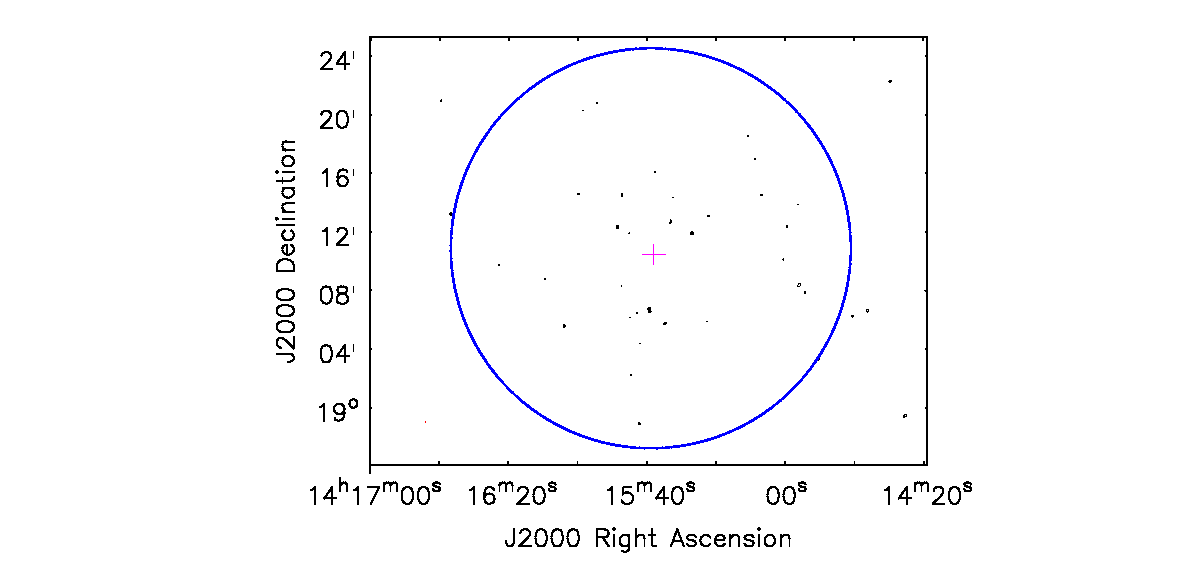
\includegraphics[trim=130pt 0pt 100pt 0pt,clip,width=15cm,height=12cm]{/home/eamon/thesis/thesis_template/4/l_thesis.ps}  
\caption[Wide field view of the VLA 20\,cm image]{Wide field view of the VLA 20\,cm CLEANed image showing the many serendipitous background sources close to Arcturus (pink cross). Many of these sources were a few orders of magnitude brighter than Arcturus at 20\,cm. CLEAN circles were placed around all these sources during interactive CLEANing. The blue circle marks the FOV (i.e., the HPBW of the primary beam) of the VLA at 20\,cm while the pink cross in the center marks the position of Arcturus. The contour levels are set at $(0.005,0.01,0.05,0.1,0.2,0.4,0.6,0.8)\times 80.3$\,mJy, where $80.3$\,mJy is the flux of the brightest source in the image.}
\label{fig:4.8}
\end{figure}

At long VLA wavelengths the primary beam becomes larger and the background sky sources become brighter. The new wide bandwidth capabilities of the VLA means that it is quite sensitive to emission far from phase center. For example, at $\sim 20$\,cm (L-band), the HPBW of the primary beam is $\sim 30^{\prime}$ and yet the primary beam gain is as much as 10\% around $1^{\circ}$ away. In Figure \ref{fig:4.8} we show a wide field view of our VLA 20\,cm image clearly showing many serendipitous sources out to and beyond the HPBW of the primary beam, all of which needed to be individually CLEANed to reduce their sidelobe contamination of the final image. For this reason the image sizes were usually set to a few times the size of the primary beam (if not too computationally expensive) so that any nearby strong serendipitous sources could be CLEANed. These images were again CLEANed interactively while taking sky curvature into account. CLEANing was carried out interactively with CLEAN circles first placed around the strongest sources in the image and then placing them around weaker sources as they appeared in the residual image. 
 
\subsection{Imaging the CARMA Data}\label{sec:4.3.2}

The CO emission around Betelgeuse is extended and has many different spatial scales. Traditional deconvolution techniques such as the CLEAN and MEM algorithms are scale-free and have no concept of source size. Both algorithms treat each pixel as an independent degree of freedom. However, adjacent pixels in an image are not independent due to the limiting resolution set by the dirty beam and the intrinsic source size. For example a Gaussian source covering 50 pixels can be characterized by only 5 parameters, not 50. The CASA multi-scale algorithm uses ``Multi-scale CLEAN'' \citep{cornwell_2008} which is a scale sensitive algorithm that employs fewer degrees of freedom to model plausible sky brightness distributions. Instead of deconvolving using just delta-functions (or pixels) as in other clean algorithms, Multi-scale CLEAN carries out the deconvolution using delta-functions and circular Gaussians of various scales. It has been shown to produce more realistic representations of the sky brightness distribution for extended complex emission than the traditional CLEAN algorithm does \citep{rich_2008}.

\begin{figure}[hbt!]
\centering 
\mbox{
\includegraphics[trim=127pt 0pt 130pt 0pt,clip,scale=0.7]{/home/eamon/thesis/thesis_template/4/thesis_clean.eps}  
\includegraphics[trim=127pt 0pt 130pt 0pt,clip,scale=0.7]{/home/eamon/thesis/thesis_template/4/thesis_multi.eps}  
}
\mbox{
\includegraphics[trim=127pt 0pt 130pt 0pt,clip,scale=0.7]{/home/eamon/thesis/thesis_template/4/thesis_clean_resid.eps}  
\includegraphics[trim=127pt 0pt 130pt 0pt,clip,scale=0.7]{/home/eamon/thesis/thesis_template/4/thesis_multi_resid.eps}  
}
\caption[Comparing CLEAN to Multi-scale CLEAN]{Comparing CLEAN to Multi-scale CLEAN using one of the combined configuration CARMA channel maps at -14.1\,km\,s$^{-1}$. The top panel shows the final deconvolved images using CLEAN (left) and Multi-scale CLEAN (right) with the emission in both maps truncated between 0 and 0.2\,Jy\,beam$^{-1}$ to enhance weak emission. Multi-scale CLEAN is more successful at recovering large-scale structure. The bottom panel shows the residual images after using CLEAN (left) and Multi-scale CLEAN (right) where the emission in both images have been truncated between 0 and 0.06\,Jy\,beam$^{-1}$. The emission appears more noise-like in the Multi-scale residual image while the CLEAN residual image contains some uncleaned flux.}
\label{fig:4.9}
\end{figure}

Multi-Scale CLEAN is really just a modification of the classical CLEAN algorithm. It assumes that sources in the sky are actually extended structures of different scales (which can include point sources), unlike the traditional CLEAN algorithm which assumes the sky is empty apart from a limited number of point sources. The function used to define the shape of the different spatial scales (usually a truncated circular Gaussian) has a finite extent and becomes a delta-function in the limit of zero scale-size. The Multi-scale CLEANing process is then as follows:
\begin{enumerate}
\item The dirty map is convolved with each scale size to create $n$ convolved images, where $n$ is the number of defined scale sizes.
\item The global scale among these images that contains the maximum total flux has its position, flux, and scale size recorded.
\item The pre-computed scale in which the peak was found, is convolved by the dirty beam, multiplied by some gain factor, and the subtracted from all the images made in the first step.
\item The subtracted component and its scale size is stored in a table.
\item Steps $1-4$ are repeated until a flux threshold is reached in one of the residual images.
\end{enumerate}
The new model is then convolved with a CLEAN beam and the residuals are added to it to get the restored image.

The combined CARMA configuration image cubes were Multi-scale CLEANed down to the 3$\sigma _{\rm{rms}}$ threshold. Natural weighting was applied to the $u-v$ data to optimize the sensitivity for the weak CO emission and the CLEAN region was set to be about the size of the HPBW of the primary beam. The Multi-scale algorithm  within CASA was set to four unique scales; the largest corresponding to the largest structures visible in individual channel maps. Each scale was approximately set to three times smaller than the preceding scale and a zero-scale was included to account for point sources. In Figure \ref{fig:4.9} we plot one channel from the final restored image cube and compare this to the same channel from an image cube that was deconvolved using the traditional CLEAN algorithm. It can clearly be seen that Multi-scale CLEAN produces more extended emission around the star. This is because Multi-scale CLEAN removes large-scale structure before finer details while the CLEAN algorithm cannot distinguish noise peaks from faint real signals \citep{rich_2008}. We also include the resultant residual images from both algorithms in the bottom panel of Figure \ref{fig:4.9}. The CLEAN residual image still contains some uncleaned flux while the emission appears more noise-like in the Multi-scale residual image.
%%!TEX root = ../thesis.tex
%Adding the above line, with the name of your base .tex file (in this case "thesis.tex") will allow you to compile the whole thesis even when working inside one of the chapter tex files

\chapter{Multi-wavelength Study of Betelgeuse's Outer Atmosphere} \label{chap:5}

\section{CO molecules in the CSE of Betelgeuse}\label{sec:5.1}
The CSE of Betelgeuse ($\alpha$ Ori) is a proving ground for ideas and theories of mass loss from oxygen-rich M-type supergiants. Currently it is losing mass at a respectable rate $\sim 2\times 10^{-6} \ M_{\odot}$ yr${}^{-1}$ \citep{harper_2001}, as it has been over the past $\sim$ 1000 years. Most of the optically thin silicate dust lies beyond $\sim 46$ stellar radii \citep{danchi_1994} and dust is, therefore, unlikely to be responsible for the bulk mass loss. This raises the important point that if the mass loss from Betelgeuse is not a result of dust then perhaps the same mechanisms that are responsible might also be active in the more dusty later M-type supergiants. Radiation pressure on atoms and molecules is another potential contributing candidate as a mass loss mechanism and so spatial and dynamical studies of molecules are a fruitful line of investigation, especially in relation to eventual formation of dust. Such studies also allow us to calculate the time scales on which certain mass loss episodes have occurred, and these can then be compared to the time scales of potential mass-loss initiators such as convection or magnetic dynamo cycles.

\begin{figure}[!ht]
\centering 
          \includegraphics[trim=30pt 130pt 30pt 100pt,clip,width=14.5cm,height=13.0cm]{/home/eamon/thesis/thesis_template/5/bernat.ps}
\caption[The first detection of the ro-vibrational absorption lines of $\rm{{}^{12}C^{16}O}$ and $\rm{{}^{13}C^{16}O}$]{The first detection of 4.6\,$\mu$m ro-vibrational absorption lines of $\rm{{}^{12}C^{16}O}$ and $\rm{{}^{13}C^{16}O}$ by \cite{bernat_1979} who used them to probe the physical conditions of the CSE. They identified the two absorption features as two distinct structures within the overall outflow. The units of the x-axis are cm$^{-1}$.}
\label{fig:5.1}
\end{figure}

The study of CO molecules in the CSE of Betelgeuse began with the detection of 4.6\,$\mu$m ro-vibrational absorption lines of $\rm{{}^{12}C^{16}O}$ and $\rm{{}^{13}C^{16}O}$ by \cite{bernat_1979} who identified two absorption features shown in Figure \ref{fig:5.1}, implying two distinct structures within the overall outflow. One component, known as S1, has a Doppler shift of $9\>{\rm km\>s}^{-1}$ towards us with T$_{\rm{exc}}\,\simeq\,200\,\rm{K}$, $v_{\rm{turb}}\,\simeq\,4$\,km\,s${}^{-1}$ and N$_{\rm{^{12}C^{16}O}}=4.7\times 10^{17}\>{\rm cm}^{-2}$. The second faster component, known as S2, has a Doppler shift of $16\>{\rm km\>s}^{-1}$ towards us with T$_{\rm{exc}} \simeq$ 70 $\rm{K}$, $v_{\rm{turb}}\simeq 1$\,km\,s${}^{-1}$ and N$_{\rm{^{12}C^{16}O}}=1.2\times 10^{16}\>{\rm cm}^{-2}$. The S1 feature with its higher column density was well known from atomic absorption line studies \citep[e.g.][]{weymann_1962} and both features had been detected in high spectral resolution atomic Na and K absorption profiles \citep{goldberg_1975}.

\begin{figure}[!ht]
\centering 
\mbox{
          \includegraphics[trim=40pt 240pt 50pt 230pt,clip,width=7.0cm,height=6.0cm]{/home/eamon/thesis/thesis_template/5/huggins_1987.ps}
          \includegraphics[trim=30pt 250pt 20pt 200pt,clip,width=7.5cm,height=6.5cm]{/home/eamon/thesis/thesis_template/5/huggins_1994.ps}
          }
\caption[Previous CO$J= 2-1$ rotational emission line profiles]{Previous single dish CO($J= 2-1$) rotational emission line profiles of Betelgeuse. \textit{Left:} \cite{huggins_1987} line profile using a HPBW of 32$\arcsec$. They found some evidence for an S2 radius of about $16\arcsec$. \textit{Right:} The line of \cite{huggins_1994} looks very similar even using a smaller HPBW in conflict with the findings of \cite{huggins_1987}. Velocities are plotted in the local standard of rest (LSR) frame.}
\label{fig:5.2}
\end{figure}

$\rm{{}^{12}C^{16}O}$ was subsequently detected at 230\,GHz in the $J= 2-1$ rotational emission line by \cite{knapp_1980}, although a search at 86\,GHz for SiO($J= 2-1$) by \cite{lambert_1978} had been unsuccessful. The weaker $\rm{{}^{12}C^{16}O}$($J=1-0$) line was tentatively detected by \cite{knapp_1985} with a 7\,m dish which had a HPBW of 100$\arcsec$. \cite{huggins_1987} presented a higher signal-to-noise $\rm{{}^{12}C^{16}O}$($J= 2-1$) observation of Betelgeuse's CSE with a HPBW of 32$\arcsec$ shown in Figure \ref{fig:5.2} and found some evidence for an S2 radius of about $16\arcsec$ by comparing the  $(2-1)/(1-0)$ intensities. However,  a 30\,m IRAM $J= 2-1$ line profile was later presented by \cite{huggins_1994} and as can be seen in Figure \ref{fig:5.2} looked remarkably similar, even though it was observed with a smaller 12$\arcsec$ HPBW. The profile did not show the horned wing signature expected if it had been resolved as discussed in Chapter 1, apparently in conflict with the previous S2 radius estimate. These single dish line profiles also showed no signature of the slower S1 shell and so questions remained about the spatial extent of these two distinct outflow components in the CSE of Betelgeuse. A sensitive high spatial resolution study of it's atmosphere was needed to untangle this puzzling evidence.

\section{Adopted Radial Velocity}\label{sec:5.2}

Before we discuss the CO($J=2-1$) spectra obtained from our multi-configuration CARMA observations discussed in Chapter 3, we begin by explaining which radial velocity value $v_{\rm{rad}}$, for Betelgeuse was used. An accurate value of $v_{\rm{rad}}$ is necessary when plotting the spectra of any star with respect to its center of mass rest frame, as we do for all spectra in this chapter. Plotting spectra in this frame of reference is intuitive as it allows the reader to immediately see the gas expansion velocity relative to the photosphere. A positive $v_{\rm{rad}}$ denotes recession (i.e., redshifted lines) while a negative $v_{\rm{rad}}$ denotes advancement (i.e., blueshifted lines).

Betelgeuse is a  semi-regular variable and its radial velocity exhibits variability on time scales ranging from short 1.5 year periods as suggested by \cite{stebbins_1931} to longer 5.8 year periods \citep{spencer_jones_1928,smith_1989}. 
\cite{stothers_1971} interpreted the long period as being the convective turnover time of giant convection cells on the stellar surface while \cite{dupree_1990} attribute the shorter period with pulsation. Betelgeuse's radial velocity amplitudes are also known to vary by at least $\pm 3\>{\rm km\>s}^{-1}$ \citep{smith_1989} making it difficult to determine a precise value for the stellar center of mass radial velocity. In Figure \ref{fig:5.3} we plot the radial velocity data and the corresponding model derived in the classical paper by \cite{sanford_1933} which is based on observations spanning 1923 to 1931. We have also extrapolated the model back to show that it matches the earlier data of \cite{bottlinger_1911} and \cite{spencer_jones_1928} quite well, as shown in Figure \ref{fig:5.3}. \cite{goldberg_1984} has also shown that the model of \cite{sanford_1933} can be extrapolated forward to give a reasonable fit to his measurements. In this study we adopt a heliocentric radial velocity of $+20.7\>{\rm km\>s}^{-1}$;  a method used by \cite{weymann_1962} and \citet{harper_2008} and is based on the mean values of \cite{spencer_jones_1928} and \cite{sanford_1933}. 

\begin{figure}[!ht]
\centering 
\mbox{
          \includegraphics[trim=0pt 0pt 0pt 50pt,clip,angle=90,height=7.0cm,width=7.3cm]{/home/eamon/thesis/thesis_template/5/vrad1.ps}
          \includegraphics[trim=0pt 0pt 0pt 50pt,clip,angle=90,height=7.0cm,width=7.3cm]{/home/eamon/thesis/thesis_template/5/vrad2.ps}
          }
\caption[Radial velocity data and model for $\alpha$ Ori.]{The radial velocity model of \cite{sanford_1933} along with measurements from \cite{bottlinger_1911}, \cite{spencer_jones_1928}, and \cite{sanford_1933} spanning from $1897 - 1931$. In this study we use $+20.7\>{\rm km\>s}^{-1}$ which is the mean value from the models of \cite{spencer_jones_1928} and \cite{sanford_1933}.}
\label{fig:5.3}
\end{figure}

\section{CARMA CO($J=2-1$) Spectra}\label{sec:5.3}
The spectrum for each individual configuration image cube (which are composed of all the appropriate configuration tracks listed in Table \ref{tab:3.3}) along with the multi-configuration image cube can be used to obtain information on the kinematics of the S1 and S2 flows. In particular it is of interest to see how the CO($J=2-1$) line profile changes when observed  with different array configurations because, prior to this study, the line had only every been observed with single dish antennas. The spectra corresponding  to the C, D, and E configuration image cubes are plotted in Figure \ref{fig:5.4} for both the high ($0.65\>{\rm km\>s}^{-1}\> \rm{bin}^{-1}$) and low ($1.3\>{\rm km\>s}^{-1}\> \rm{bin}^{-1}$) spectral resolution data and were obtained by integrating all emission within a circular area of radius 5$\arcsec$ centered on the source. The high and low spectral resolution modes allow two independent sets of spectra to be measured for each observation and thus provide a good check on the data quality. The high resolution  spectra (channel width = $0.65\>{\rm km\>s}^{-1}$) give the best measure of S1 and S2 kinematics and therefore all outflow velocities are derived from these spectra.

\begin{figure}[!ht]
\centering 
\includegraphics[trim=80pt 60pt 40pt 80pt, clip, width=9.0cm, height=12.0cm]{/home/eamon/thesis/thesis_template/5/f1.eps}
\caption{Spectra integrated over a radius of 5$\arcsec$ for each array configuration image cube. The blueshifted emission component between $-16.0\>{\rm km\>s}^{-1}$ and $-10.0\>{\rm km\>s}^{-1}$ is almost resolved out in the C configuration image cube spectrum. The red and blue lines correspond to the high and low spectral resolution data respectively.}
\label{fig:5.4}
\end{figure}

The E configuration image cube spectrum has a total line width of $29.2\>{\rm km\>s}^{-1}$ and the low spectral resolution profile contains a steep blue wing emission feature between $-16.0\>{\rm km\>s}^{-1}$ and $-11\>{\rm km\>s}^{-1}$ and a more flat-topped feature between $-10.3\>{\rm km\>s}^{-1}$ and $-13.2\>{\rm km\>s}^{-1}$. This steep emission wing shows that the turbulence in the flow is less than or equal to the velocity bin size. The blue wing in the high resolution profile matches the lower resolution profile well but the  remainder of the profile looks more complex than the flat-topped feature seen in the lower resolution profile. The line profile shape has been well documented by previous single dish observations (e.g., Figure \ref{fig:5.2}) and, out of our three individual configuration spectra, we expect the most compact E configuration spectra to resemble these single dish measurements the closest due to its better sampling of the inner u-v plane and consequent sensitivity to extended structures. This indeed turns out to be the case when we compare our three individual configuration spectra to those previous single dish profiles. The blue wing emission feature appears again in the D configuration spectrum at the same velocities as those in the E configuration spectrum but the remainder of the profile appears quite different. Between $-10.3\>{\rm km\>s}^{-1}$ and $+13.2\>{\rm km\>s}^{-1}$ the D configuration spectrum is dominated by a blue wing at $\sim$ $-10.0\>{\rm km\>s}^{-1}$, a red wing at $\sim$ $+13.0\>{\rm km\>s}^{-1}$ and an emission feature at $\sim$ $0\>{\rm km\>s}^{-1}$. The large drop in emission at certain velocities in the D configuration spectrum is probably a result of the lower sensitivity to large scale structure in comparison to the E configuration as shown in Table \ref{tab:3.2}.

The line profile has a much lower flux in the high spatial resolution C configuration spectrum due to its lack of sensitivity to extended structure. The blueshifted emission feature located between $-16.0\>{\rm km\>s}^{-1}$ and $-11.0\>{\rm km\>s}^{-1}$ in the E and D configuration spectra is almost completely spatially filtered by the extended C configuration. This component of the line has previously been associated with the outer S2 flow \citep{huggins_1987} and as the majority of it has been spatially filtered by our C configuration we expect even less contribution from the S2 flow at lower absolute velocities still. For the redshifted line emission we again expect the majority of the S2 contribution to be spatially filtered, so we conclude that the majority of the emission in the C configuration spectrum emanates from the inner S1 flow. The spectrum is double peaked with the blue and redshifted wings extending to $-9.0\>{\rm km\>s}^{-1}$ and $+10.6\>{\rm km\>s}^{-1}$ respectively, and we define these as the outflow velocities of S1. As discussed in Chapter \ref{chap:3} the C configuration has a resolving out scale of $\sim$ 6$\arcsec$ at 1.3 mm and so is not sensitive to angular scales larger than this. If the emission between $-9.0\>{\rm km\>s}^{-1}$ and $+10.6\>{\rm km\>s}^{-1}$ in the C configuration spectrum appeared as a flat topped profile then we could conclude that the S1 flow lies within a radius of 3$\arcsec$ from the star. Clearly however, the lower absolute velocity components of this profile have been spatially filtered so we conclude that the radial extent of the S1 from the star is greater than 3$\arcsec$. If we assume that the S1 flow would produce a 19.6 km s$^{-1}$ wide top-hat line profile of 2 mJy were it not for the resolving out effects of the interferometer, its integrated line flux is
\begin{equation}
F_{\rm{tot\,S1}}=F_{\nu}\times \left(\frac{\Delta v}{\lambda}\right)= 3.1 \times 10{}^{-19}\,\rm{W\,m}{}^{-2}.
\label{eq:5.1}
\end{equation}

To obtain the most robust value for the S2 outflow velocities we examine the high spectral resolution multi-configuration image cube spectrum which is composed of all tracks from all three configurations. It is worth stressing that by analyzing the multi-configuration image cube we make the assumption that the physical properties of all three components (i.e. $\alpha$ Ori, S1 and S2) have not changed over the total observation period (i.e. $\sim$ 2.5 yr). The profile is found to have a total linewidth of 28.6 $\pm$ $0.7\>{\rm km\>s}^{-1}$, which is in close agreement with previous single dish observations of the line where values of 30.6 $\pm$ $2.5\>{\rm km\>s}^{-1}$ and $28.6\>{\rm km\>s}^{-1}$ were reported by \cite{knapp_1980} and \cite{huggins_1987} respectively. The centroid velocity of the spectrum is  $-1.1 \pm 0.7$ km s$^{-1}$ ($\rm{v_{\rm{lsr}}}$ = 3.7 $\pm$ $0.7\>{\rm km\>s}^{-1}$) which is again in close agreement with \cite{knapp_1980} and \cite{huggins_1987} values of $\rm{v_{lsr}}$ = 3.0 $\pm$ $2.5\>{\rm km\>s}^{-1}$ and $\rm{v_{lsr}}$ = 3.7 $\pm$ $0.4\>{\rm km\>s}^{-1}$ respectively. We use Equation \ref{eq:5.1} to find the integrated line flux to be 1.5 $\times 10^{-18}$\,W\,m$^{-2}$, of which approximately 20\% emanates from the S1 flow.

The outflow velocities of S2 are $-15.4\>{\rm km\>s}^{-1}$ and $+13.2\>{\rm km\>s}^{-1}$ which, like the S1 flow, are slightly asymmetric but in the opposite sense. Note that the S1 and S2 outflow velocities are dependent on the adopted radial velocity of Betelgeuse. If for instance, we instead adopt a radial velocity of 21.9 km s${}^{-1}$ \citep{famaey_2005} then the the S2 outflow velocities become even more asymmetric (-16.6 and $+12.0\>{\rm km\>s}^{-1}$) while the S1 outflow becomes less so (-10.2 and $+9.4\>{\rm km\>s}^{-1}$). Both S1 and S2 therefore cannot have spherically symmetric outflow velocities regardless of the adopted stellar radial velocity. Adopting a mass of 18\,$M_{\odot}$ and a radius of 950\,$R_{\odot}$ \citep{harper_2008} then the escape velocity for Betelgeuse is $85\>{\rm km\>s}^{-1}$ which is much greater than the S1 and S2 outflow velocities. This indicates that the majority of the stellar mass loss mechanism's energy goes into lifting the CO molecules out of the gravitational potential and not into their outflow velocities. These outflow velocities are greater than the adiabatic hydrogen sound speed, which, if we assume that the gas temperature is the same as the excitation temperature, are $1.7\>{\rm km\>s}^{-1}$ and $1\>{\rm km\>s}^{-1}$ for S1 and S2 respectively. 

\begin{figure}[!ht]
\centering 
\includegraphics[trim=20pt 180pt 40pt 0pt, clip, angle=90, width=14.0cm, height=12.0cm]{/home/eamon/thesis/thesis_template/5/f2.eps}
\caption{Spectral profiles of the low spectral resolution multi-configuration image cube for circular extraction areas of radius 1$\arcsec$, 2$\arcsec$, 4$\arcsec$, 6$\arcsec$, 8$\arcsec$, and 10$\arcsec$. The signal-to-noise of the line profile reduces at larger extraction areas as more noise is included from the outer regions of the channel maps.}
\label{fig:5.5}
\end{figure}

The spectra in Figure \ref{fig:5.5} are taken from the low resolution multi-configuration image cube using circular extraction areas ranging in radius from 1$\arcsec$ to 10$\arcsec$ and demonstrates how the line profile changes over these different extraction areas. The most striking change in the line profile is the change in appearance of the extreme blue wing. At small extraction radii where we sample the most compact emission, the feature is weak in comparison to the rest of the line but becomes more dominant as we begin to sample more of the extended emission. This indicates that even the high absolute velocity components of the S2 flow have extended emission and this is why they are almost completely spatially filtered by CARMA's C configuration. The large reduction of flux at $-11\>{\rm km\>s}^{-1}$ suggests that there is more material moving towards the observer than at other lower absolute velocities indicating a non-isotropic (or non-spherical) S2 flow. This suggests a more sheet like (flatter) structure rather than a spherical cap.

\section{Individual Configuration Image Cubes}\label{sec:5.4}

We created three image cubes for each configuration by concatenating all good tracks together per configuration. The gradual formation of a ring type structure as one goes from high absolute velocities to lower absolute velocities indicative of a shell was not seen in any of these three image cubes. However, an additional spatially unresolved source was clearly detected in a number of the D configuration image cube maps (both high and low spectral resolution). The component is present in five continuous channel maps between $\sim$ $-4.0\>{\rm km\>s}^{-1}$ and $+2.4\>{\rm km\>s}^{-1}$ and is located $\sim$ 5$\arcsec$ S-W of $\alpha$ Ori. Its peak emission lies at $\sim$ $0\>{\rm km\>s}^{-1}$ and has a flux density of 1.8\,mJy which is approximately 60$\%$ of the total source flux density at this velocity. The middle row in Figure \ref{fig:5.6} are two of these D configuration channel maps which clearly show this discrete source. The contour levels are set at the $4\sigma$ level so the detection of the second source in the D configuration is significant. The corresponding channel maps in the E configuration image cube show extended emission out to ~8$\arcsec$ in the same S-W direction as can be seen in the lower panel of Figure \ref{fig:5.6}. There is only weak emission detected in the same position in the corresponding C configuration channel maps, probably due to the lower sensitivity resulting from the smaller HPBW (i.e. the flux is diluted). This discrete second source thus has the effect of adding extra emission to the corresponding multi-configuration image cube spectrum at the low absolute velocities where it is present. The presence of this addition source at these low absolute velocities is probably one of the reasons why \cite{huggins_1994} did not detect a horned shaped spectrum with his 12$\arcsec$ HPBW. We also note that that there is a weaker emission feature 7$\arcsec$ north north-west of $\alpha$ Ori in these maps also which too can be seen in Figure \ref{fig:5.6}. 

\begin{figure}[htp]
\mbox{
          \includegraphics[trim=0pt 0pt 10pt 10pt,clip,height=6.2cm,width=14.0cm]{/home/eamon/thesis/thesis_template/5/c.ps}
          }
\mbox{
          \includegraphics[trim=0pt 0pt 10pt 10pt,clip,height=6.2cm,width=14.0cm]{/home/eamon/thesis/thesis_template/5/d.ps}
          }
\mbox{
          \includegraphics[trim=0pt 0pt 10pt 10pt,clip,height=6.2cm,width=14.0cm]{/home/eamon/thesis/thesis_template/5/e.ps}
          }          
\caption[Discrete sources in individual configuration image cubes]{Two channel maps from each of the three individual configuration image cubes. A spatially unresolved source is present in five continuous channel maps between $\sim$ $-4.0\>{\rm km\>s}^{-1}$ and $+2.4\>{\rm km\>s}^{-1}$ and is located $\sim$ 5$\arcsec$ S-W of $\alpha$ Ori. Contour levels begin at $4\sigma$ where $1\sigma$ is the rms channel noise. The restoring beam is shown in green in the lower left corner of each map.}
\label{fig:5.6}
\end{figure}

\section{Multi-configuration Image Cube Inspection}\label{sec:5.5}

A subset of the blueshifted velocity channel maps of the low spectral resolution multi-configuration image cube is presented in Figure \ref{fig:5.7}. The first channel map at $-17.9\>{\rm km\>s}^{-1}$ shows just the compact unresolved continuum emission with no extended emission present. Between $-16.7\>{\rm km\>s}^{-1}$ and $-9.0\>{\rm km\>s}^{-1}$ we see evidence for the development of a classical shell signature for the S2 flow. We first sample the highest velocity components where the emission is relatively compact (i.e. between $-16.7\>{\rm km\>s}^{-1}$ and $-12.9\>{\rm km\>s}^{-1}$) and then sample lower radial velocity components where S2 becomes a faint ring (i.e. between $-11.6\>{\rm km\>s}^{-1}$ and $-9.0\>{\rm km\>s}^{-1}$). At lower velocities again, these rings disappear into the noise of the maps and possibly extend out beyond the primary beam at zero velocity when the rings should have maximum spatial extent. The emission from the channel maps between $-15.3\>{\rm km\>s}^{-1}$ and $-11.6\>{\rm km\>s}^{-1}$ correspond to all the emission in the extreme blue wing component of the multi-configuration image cube line profile discussed in \S3.1. We can see in Figure \ref{fig:5.7} that all of this emission is greater than the C configuration resolving out scale of $\sim 6\arcsec$, therefore confirming that our C configuration line profile is mainly composed of S1 emission. The shell formation signature of S2 is also apparent in the redshifted velocity channel maps between $+7.5\>{\rm km\>s}^{-1}$ and $+13.8\>{\rm km\>s}^{-1}$ but the emission appears weaker and the rings fainter therefore indicating that S2 is somewhat fragmented. 

%\begin{figure}[htp]
%\centering
%\mbox{
%          \includegraphics[trim=130pt 15pt 120pt 15pt,clip,scale=0.55]{/home/eamon/thesis/thesis_template/5/1.eps}
%          \includegraphics[trim=180pt 15pt 120pt 15pt,clip,scale=0.55]{/home/eamon/thesis/thesis_template/5/2.eps}
%         \includegraphics[trim=260pt 230pt 200pt 270pt,clip,scale=0.4]{/home/eamon/thesis/thesis_template/5/color_wedge.ps}
%          }
%\mbox{
%          \includegraphics[trim=130pt 15pt 120pt 15pt,clip,scale=0.55]{/home/eamon/thesis/thesis_template/5/3.eps}
%          \includegraphics[trim=180pt 15pt 120pt 15pt,clip,scale=0.55]{/home/eamon/thesis/thesis_template/5/4.eps}
%          \includegraphics[trim=260pt 230pt 200pt 270pt,clip,scale=0.4]{/home/eamon/thesis/thesis_template/5/color_wedge.ps}
%          }
%\mbox{
%          \includegraphics[trim=130pt 15pt 120pt 15pt,clip,scale=0.55]{/home/eamon/thesis/thesis_template/5/5.eps}
%          \includegraphics[trim=180pt 15pt 120pt 15pt,clip,scale=0.55]{/home/eamon/thesis/thesis_template/5/6.eps}
%          \includegraphics[trim=260pt 230pt 200pt 270pt,clip,scale=0.4]{/home/eamon/thesis/thesis_template/5/color_wedge.ps}
%          }
%\mbox{
%          \includegraphics[trim=130pt 15pt 120pt 15pt,clip,scale=0.55]{/home/eamon/thesis/thesis_template/5/7.eps}
%          \includegraphics[trim=180pt 15pt 120pt 15pt,clip,scale=0.55]{/home/eamon/thesis/thesis_template/5/8.eps}
%          \includegraphics[trim=260pt 230pt 200pt 270pt,clip,scale=0.4]{/home/eamon/thesis/thesis_template/5/color_wedge.ps}
%          }                           
%\caption[Channel maps from the multi-configuration image cube]{8 channel maps from the multi-configuration image cube ($\Delta v$ = $1.3\>{\rm km\>s}^{-1}$). The peak emission has been cut at 0.2 Jy beam${{}^{-1}}$ to emphasize the fainter emission. The map at $-17.9$ km s$^{-1}$ is the star in the continuum while the blue wing of the line starts at $-16.7$ km s$^{-1}$. The formation of a weak ring-like structure is seen as one goes from high absolute velocities to lower ones.}
%\label{fig:5.7}
%\end{figure}

The multi-configuration maps also show the central compact emission from the S1 flow at velocities between $-10.3\>{\rm km\>s}^{-1}$ and $+11.3\>{\rm km\>s}^{-1}$. This S1 emission can be seen in the final two maps of Figure \ref{fig:fig3} as a central slightly elongated emission feature surrounded by the fainter rings of the S2 flow. In the maps where both S1 and S2 are present the emission from S1 appears brighter than the emission from S2. The spatial extent of the S1 flow varies from channel map to channel map but appears to be larger than the 2$\arcsec$ value given by \cite{smith_2009}, who observed off-star wind scattered ro-vibration CO lines. 

\section{Multi-configuration Image Cube Analysis}\label{sec:5.6}

\subsection{Spatial Extent of S2}
The spatial extent of the S1 and S2 flows around Betelgeuse were not directly determined from either the CO infrared absorption spectra of \cite{bernat_1979} or previous CO single dish radio observations \citep{knapp_1980, huggins_1987, huggins_1994}. Our low spectral resolution multi-configuration image cube has sufficient spatial resolution and signal-to-noise to make direct estimates of the maximum radius of both flows. The outer S2 flow is not seen in the low absolute velocity channel maps where its spatial extent is maximum and either lies outside of the primary beam or is lost into the noise near the edge of the maps. Therefore we cannot make a direct measurement of its maximum size. However, we can derive the maximum outer scale of the S2 flow by looking at the spatial scales of the S2 flow in the higher absolute velocity maps where S2 is present. 

\begin{figure}[!ht]
\centering 
\includegraphics[trim=0pt 320pt 50pt 240pt, clip, scale=0.8]{/home/eamon/thesis/thesis_template/5/shell_size_est.ps}
\caption[Geometry of a spherical symmetric flow.]{Geometry of a spherical symmetric flow used to derive the spatial extent of the S2 flow. By measuring the spatial extent of S2 (i.e., $R_{\rm{S2}}\rm{sin}\theta$) as a function of channel/velocity (i.e., $V_{\rm{S2}}\rm{cos}\theta$) the maximum spatial extent of the S2 flow can be derived.}
\label{fig:5.8}
\end{figure}

If we assume that S2 is spherically symmetric with an outer radius $R_{\rm{S2}}$, and is undergoing steady expansion with velocity $V_{\rm{S2}}$, then its geometry is described by Figure \ref{fig:5.8}. As we sample the line at different velocities, the spatial extent of S2 changes and gets progressively larger at lower absolute velocities as shown in Figure \ref{fig:5.7}. We define the spatial extent of S2 in each map as
\begin{equation}
r_{\rm{chan}}=R_{S2}\times \rm{sin}\mathrm{\theta}
\label{eq:5.6a}
\end{equation}
which can be measured in many of the channel maps. Each of these channel maps has an associated velocity $V_{\rm{chan}}$, which we know, and is related to the actual velocity of the S2 flow by
\begin{equation}
V_{\rm{chan}}=V_{S2}\times \rm{cos}\mathrm{\theta}.
\label{eq:5.6b}
\end{equation}
Combining Equations \ref{eq:5.6a} and \ref{eq:5.6b} via the angle dependence, gives the following equation which contains $R_{\rm{S2}}$ as the only unknown parameter,
\begin{equation}
r_{\rm{chan}}= R_{\rm{S2}}\times \rm{sin}\left[\rm{cos}^{-1}\left(\frac{\mathit{V}_{chan}}{\mathit{V}_{S2}}\right) \right].
\label{eq:5.6c}
\end{equation} 

We now use Equation \ref{eq:5.6c} to estimate the maximum projected spatial extent of S2 which occurs at zero velocity. An estimate of the S2 radius per channel ($r_{\rm{chan}}$) was found by creating annuli of increasing radius around the central emission in each relevant line channel map of the multi-configuration image cube, extracting all flux within each annulus and then plotting these fluxes against distance from the star for each channel map as demonstrated in Figure \ref{fig:5.9}. The maximum of these resultant curves was then deemed to be the maximum radius of S2 per channel map. Figure \ref{fig:5.10} shows these data over-plotted with two model outflows which were created using Equation \ref{eq:5.6c}. The blueshifted data points were best fitted by a model outflow of maximum radius 17$\arcsec$ and outflow velocity $17\>{\rm km\>s}^{-1}$, while the redshifted data points were best fitted by a model outflow of maximum radius 16$\arcsec$ and outflow velocity $14\>{\rm km\>s}^{-1}$. It is worth mentioning that this estimate for the spatial extent of S2 is only weakly dependent on our adopted radial velocity value for Betelgeuse and adopting a slightly different value would simply alter the outflow velocities.

\begin{figure}
\centering 
\includegraphics[trim=0pt 0pt 0pt 0pt, clip, scale=0.65]{/home/eamon/thesis/thesis_template/5/annulus_flx_blue.eps}
\caption[Deriving $R_{\rm{chan}}$ per channel map]{Deriving $R_{\rm{chan}}$ per channel map. The maximum of the curves representing the integrated flux as a function of distance from the star was deemed as the size of S2 in each channel map.}
\label{fig:5.9}
\centering 
\includegraphics[trim=0pt 0pt 0pt 0pt, clip, scale=0.65]{/home/eamon/thesis/thesis_template/5/f13.eps}
\caption[S2 radius as a function of channel velocity]{The derived S2 radius as a function of velocity (red points) overplotted with two model outflows. The blueshifted model (left) corresponds to an outflow with a maximum radius of 17$\arcsec$ and a velocity of $16.7\>{\rm km\>s}^{-1}$ while the redshifted model (right) corresponds to an outflow with a maximum radius of 16$\arcsec$ and a velocity of $13.8\>{\rm km\>s}^{-1}$. Note: The line profile is $1.9\>{\rm km\>s}^{-1}$ wider in the low resolution image cube ($\Delta v$ = $1.3\>{\rm km\>s}^{-1}$) than in the high resolution image cube.}
\label{fig:5.10}
\end{figure}

\subsection{Intensity distribution of CO}
In the left column of Figure \ref{x} we investigate the intensity distribution of CO emission as a function of projected radius, R, for both the S1 and S2 flows. From our discussions in \S \ref{results1} we can assume that all line emission between -15.4 $\rightarrow$ $-10.3\>{\rm km\>s}^{-1}$ and +12.4 $\rightarrow$ $+13.8\>{\rm km\>s}^{-1}$ emanates solely from the S2 flow. Using the low spectral resolution multi-configuration image cube we integrate the surface brightness over these channels and find that the intensity fall-off is proportional to R${}^{-1}$ (Figure \ref{fig:fig6}: \textit{top}). To investigate the S1 flow intensity distribution around $\alpha$ Ori we integrate the surface brightness over the channels between -9 $\rightarrow$ $+10.6\>{\rm km\>s}^{-1}$. Although these channels contain emission from both S1 and S2, most of the S2 emission here will have larger projected radii and thus the majority of the inner emission should emanate from the S1 flow.  Between 0.5$\arcsec$ and 4$\arcsec$ from the star the intensity is again found to be proportional to R${}^{-1}$ (Figure \ref{fig:fig6}: \textit{bottom}). Such an intensity distribution is expected for an optically thin homogeneous constant velocity outflow with $\rho \propto 1/\rm{R^{2}}$. Beyond 4$\arcsec$ the intensity fall off is more rapid and is close to a R${}^{-2}$ distribution which may mark the initiation of the current epoch of mass loss.

\begin{figure}[hbt!]
%\centering
\mbox{
          \includegraphics[scale=0.42]{/home/eamon/thesis/thesis_template/5/f14.eps}
          \includegraphics[trim=30pt 0pt 0pt 0pt, clip, scale=0.42]{/home/eamon/thesis/thesis_template/5/f15.eps}
          }
\\
\mbox{
          \includegraphics[scale=0.42]{/home/eamon/thesis/thesis_template/5/f16.eps}
          \includegraphics[trim=30pt 0pt 0pt 0pt, clip, scale=0.42]{/home/eamon/thesis/thesis_template/5/f17.eps}

          }
\\
\caption{\textit{Left Column:} Surface Brightness as a function of projected radius on sky, R (red line). The emission has been extracted from the low spectral resolution multi-configuration image cube and is integrated over the channels where S1 is present (bottom) and over the channels where only S2 is present (top). Intensity proportional to R${}^{-1}$ and R${}^{-2}$ is also shown for comparison. \textit{Right Column:} The corresponding visibility amplitude as a function of u-v distance (q) of both outflows can be modeled well by a R${}^{-1}$ fall off in intensity. The error bars in all plots represent the standard error of the mean.}
\label{fig:5.11}
\end{figure}

Insight can also be gained into how the intensity varies on different size scales by conducting analysis in the u-v plane and plotting the visibility amplitude of $\alpha$ Ori against u-v distance. The result of this is shown in the right column of Figure \ref{fig:fig6} where the same channels corresponding to the S1 and S2 flows have been used. The data are azimuthally averaged, and have been binned to produce one data point per k$\lambda$. The result for both the S1 and S2 data is a steep drop-off in visibility amplitude over a relatively short u-v distance, signaling that the sources are well resolved. Both sets of visibility data agree with an intensity proportional to $(a^2 + R^2){}^{-1/2}$, where $a$ is an inner spatial limit. This is because the Hankel transform of this function is $q^{-1}e^{-2\pi aq}$ \citep{2000fta..book.....B}, where q is the u-v distance, and a vertically scaled version of this function is shown to match the visibility data very well in Figure \ref{fig:fig6}. As analysis in both the sky and u-v plane indicate the intensity of both flows is proportional to R${}^{-1}$ we conclude that when azimuthally averaged, both outflows are  consistent with an optically thin and quasi-steady flow which is in agreement with \cite{2009AJ....137.3558S} (i.e. S1) and \cite{2002A&A...386.1009P} (i.e. S2). 

\subsection{Spatial Extent of S1}
An exact determination of the maximum spatial extent of the S1 flow is more difficult as we do not see the classical shell formation signature for it as we sample across velocities, like we do for S2. Instead its spatial extent varies over the channel maps with evidence of discrete clumps being present in many of these maps. At 20\% of maximum emission in the integrated intensity S1 map (i.e. composed of all channels between -9 $\rightarrow$ $+10.6\>{\rm km\>s}^{-1}$) the S1 flow extends out to a mean distance of $\sim$ 4$\arcsec$ and is even more extended in the S-W direction due to the presence of the second emission feature in the compact configuration data sets. The HPBW of 0.9$\arcsec$ is not sufficient to determine whether the S1 flow is discrete or an extension of the current wind phase seen in ultraviolet spectra, e.g., \cite{1997ApJ...479..970C}, and cm-radio continuum interferometry \citep{1998Natur.392..575L, harper_2001}.

Graham's proceedings
\section{Continuum Flux Densities}\label{sec:5.7}
In Table \ref{tab:5.1} we show the derived continuum flux densities for each of the three configuration image cubes and also the multi-configuration image cube. The high spectral resolution ($\Delta v$ = $0.65\>{\rm km\>s}^{-1}$) image cubes were just wide enough to image the CO line but were too narrow to make accurate estimates of the continuum flux density. Therefore, all continuum flux density estimates are derived from the lower spectral resolution ($\Delta v$ = $1.3\>{\rm km\>s}^{-1}$) image cubes from which we were able to take accurate measurements at both sides of the line. We fitted elliptical Gaussians to $\sim$ 20 continuum channels using CASA's \textit{imfit} routine allowing the flux and corresponding uncertainties to be calculated. The source was unresolved in most of these continuum channels. 

\begin{table}[!hbt]
\begin{center}
\caption[CARMA Continuum Fluxes at 230 GHz]
{CARMA Continuum Fluxes at 230 GHz}
\begin{tabular}{lccc}
\hline
\hline
\rule{0pt}{2.5ex}Configuration & Restoring Beam & Flux & Uncertainty \\
 & ($\arcsec \times \arcsec$) & (mJy) & (mJy) \\
\hline
\rule{0pt}{2.5ex}C & 0.96 $\times$ 0.76 & 234 & 18\\
D & 2.33 $\times$ 1.87 & 389 & 72\\
E & 4.93 $\times$ 3.84 & 278 & 40 \\
Multi-configuration & 1.05 $\times$ 0.84 & 289 & 21\\
\hline
\rule{0pt}{2.0ex}
\end{tabular}
\label{tab:5.1}
\end{center}
\end{table}

\section{Higher CO rotational lines}\label{sec:5.8}
SOFIA, Hershel, SMA
\section{e-Merlin Results}\label{sec:5.8}
position, GMH model
\section{Multi-wavelength VLA + Pie Town Analysis}\label{sec:5.9}
\section{Q-band VLA + Pie Town Analysis}\label{sec:5.10}
%%!TEX root = ../thesis.tex
%Adding the above line, with the name of your base .tex file (in this case "thesis.tex") will allow you to compile the whole thesis even when working inside one of the chapter tex files

\chapter{Multi-wavelength Radio Continuum Emission Studies of \\ Dust-free Red Giants} \label{chap:6}

Prior to and during the early operation of the `old' VLA, a small number of single dish radio observations reported the detection of flares from single red giants (e.g., \citealt{slee_1989}). These transient radio events have never been re-observed however, even with more sensitive interferometers, suggesting that such detections were spurious (e.g., \citealt{beasley_1992}). The first definitive detection of thermal free-free emission from a luminosity class III single red giant at centimeter wavelengths was of $\alpha$ Boo at 6 cm \citep{drake_1983,drake_1986}. Since then there has been a modest number of centimeter and millimeter observations of this star. In Table \ref{tab:6.4.1} we list the majority of these observations and plot their flux densities as a function of frequency in Figure x. In comparison to other single red giants, $\alpha$ Boo had been relatively well observed at radio continuum wavelengths before this study, including detections in four VLA bands (i.e., Q, K, Ku, and C). No Ku band receivers were available during the commissioning phase of the VLA in early 2011 so we can compare three of our detections with previous ones. \\

\section{Introduction}\label{sec:6.1}
Prior to and during the early operation of the `old' VLA, a small number of single dish radio observations reported the detection of flares from single red giants (e.g., \citealt{slee_1989}). These transient radio events have never been re-observed however, even with more sensitive interferometers, suggesting that such detections were spurious (e.g., \citealt{beasley_1992}). The first definitive detection of thermal free-free emission from a luminosity class III single red giant at centimeter wavelengths was of $\alpha$ Boo at 6 cm \citep{drake_1983,drake_1986}. Since then there has been a modest number of centimeter and millimeter observations of this star. In Table \ref{tab:6.4.1} we list the majority of these observations and plot their flux densities as a function of frequency in Figure x. In comparison to other single red giants, $\alpha$ Boo had been relatively well observed at radio continuum wavelengths before this study, including detections in four VLA bands (i.e., Q, K, Ku, and C). No Ku band receivers were available during the commissioning phase of the VLA in early 2011 so we can compare three of our detections with previous ones. \\
\section{$\alpha$ Boo Radio Maps}\label{sec:6.2}
Prior to and during the early operation of the `old' VLA, a small number of single dish radio observations reported the detection of flares from single red giants (e.g., \citealt{slee_1989}). These transient radio events have never been re-observed however, even with more sensitive interferometers, suggesting that such detections were spurious (e.g., \citealt{beasley_1992}). The first definitive detection of thermal free-free emission from a luminosity class III single red giant at centimeter wavelengths was of $\alpha$ Boo at 6 cm \citep{drake_1983,drake_1986}. Since then there has been a modest number of centimeter and millimeter observations of this star. In Table \ref{tab:6.4.1} we list the majority of these observations and plot their flux densities as a function of frequency in Figure x. In comparison to other single red giants, $\alpha$ Boo had been relatively well observed at radio continuum wavelengths before this study, including detections in four VLA bands (i.e., Q, K, Ku, and C). No Ku band receivers were available during the commissioning phase of the VLA in early 2011 so we can compare three of our detections with previous ones. \\
\begin{figure}[htp]
\centering 
\mbox{
		  \includegraphics[trim=100pt 50pt 150pt 10pt,clip,width=7.5cm,height=6.0cm]{/home/eamon/thesis/thesis_template/6/atau_q_ka.ps}
          \includegraphics[trim=130pt 50pt 150pt 10pt,clip,width=7.5cm,height=6.0cm]{/home/eamon/thesis/thesis_template/6/aboo_q_ka_k.ps}
          }
\mbox{
          \includegraphics[trim=115pt 50pt 155pt 10pt,clip,width=7.5cm,height=5.8cm]{/home/eamon/thesis/thesis_template/6/atau_x_k.ps}
          \includegraphics[trim=108pt 50pt 145pt 10pt,clip,width=7.3cm,height=5.8cm]{/home/eamon/thesis/thesis_template/6/aboo_c_x.ps}
          }
\mbox{
          \includegraphics[trim=100pt 10pt 148pt 10pt,clip,width=7.5cm,height=6.4cm]{/home/eamon/thesis/thesis_template/6/atau_c_s.ps}
          \includegraphics[trim=125pt 10pt 150pt 10pt,clip,width=7.5cm,height=6.4cm]{/home/eamon/thesis/thesis_template/6/aboo_l_s_ddt.ps}
          }
\caption[xxx]{xx}
\label{fig6.3.1}
\end{figure}

\section{$\alpha$ Tau Radio Maps}\label{sec:6.3}
Prior to and during the early operation of the `old' VLA, a small number of single dish radio observations reported the detection of flares from single red giants (e.g., \citealt{slee_1989}). These transient radio events have never been re-observed however, even with more sensitive interferometers, suggesting that such detections were spurious (e.g., \citealt{beasley_1992}). The first definitive detection of thermal free-free emission from a luminosity class III single red giant at centimeter wavelengths was of $\alpha$ Boo at 6 cm \citep{drake_1983,drake_1986}. Since then there has been a modest number of centimeter and millimeter observations of this star. In Table \ref{tab:6.4.1} we list the majority of these observations and plot their flux densities as a function of frequency in Figure x. In comparison to other single red giants, $\alpha$ Boo had been relatively well observed at radio continuum wavelengths before this study, including detections in four VLA bands (i.e., Q, K, Ku, and C). No Ku band receivers were available during the commissioning phase of the VLA in early 2011 so we can compare three of our detections with previous ones. \\


\section{Results vs Previous Observations}\label{sec:6.4}
Prior to and during the early operation of the `old' VLA, a small number of single dish radio observations reported the detection of flares from single red giants (e.g., \citealt{slee_1989}). These transient radio events have never been re-observed however, even with more sensitive interferometers, suggesting that such detections were spurious (e.g., \citealt{beasley_1992}). The first definitive detection of thermal free-free emission from a luminosity class III single red giant at centimeter wavelengths was of $\alpha$ Boo at 6 cm \citep{drake_1983,drake_1986}. Since then there has been a modest number of centimeter and millimeter observations of this star. In Table \ref{tab:6.4.1} we list the majority of these observations and plot their flux densities as a function of frequency in Figure x. In comparison to other single red giants, $\alpha$ Boo had been relatively well observed at radio continuum wavelengths before this study, including detections in four VLA bands (i.e., Q, K, Ku, and C). No Ku band receivers were available during the commissioning phase of the VLA in early 2011 so we can compare three of our detections with previous ones. \\

\begin{table}[!hb]
\begin{center}
\caption[Compilation of Previous Radio Observations ($\nu \le 250$ GHz).]
{Compilation of Previous Radio Observations ($\nu \le 250$ GHz).}
\begin{tabular}{cccccc}
\hline
\hline
\rule{0pt}{2.5ex}Source & $\nu$ (GHz) & Date &  $F_{\nu}$ (mJy) & S/N & Reference\\
\hline
$\alpha$ Boo &4.9  & 1983 Jan 21 & 0.39 & 3.0 & 1 \\
&4.9  & 1983 May 20 & 0.26 & 3.3& 1 \\
&4.9  & 1983 Dec 26 & $\le$0.18$(3\sigma)$&- & 1 \\
&4.9  & 1984 Mar 17 & 0.24  & 4.8& 1 \\
&15.0 & 1984 Nov 6 & 0.68 & 7.6& 1 \\
&22.5  & 1999 Jan 06  &1.7& 8.5& 2 \\
&43.3  & 1999 Jan 06 & 3.3& 8.3& 2 \\
&43.3  & 2004 Jan 25 & 3.34& 41.8& 2 \\
&86.0  & 1985 Nov  & 21.4& 3.0& 3 \\
&108.4  & 1997 Nov - 2000 Jun & 20.1 &29.1 & 4 \\
&217.8 & 1997 Nov - 2000 Jun  & 83.5 &48.8 & 4 \\
&250.0  & 1986 Dec - 1989 Mar  & 78.0 & 9.8& 5 \\
\hline
\rule{0pt}{3ex}    $\alpha$ Tau	&4.9  & 1983 Jan 21 & $\le$0.27$(3\sigma)$&-& 1 \\
&4.9  & 1984 Nov 6 & $\le$0.22$(3\sigma)$&-& 1 \\
&5.0  & 1997 Sep 27 & $\le$0.07$(3\sigma)$	&-& 6 \\
&8.5  & 1997 Sep 27 & 0.28 	&9.3	& 6 \\
&14.9 & 1997 Sep 27 & 0.95 	&11.9	& 6 \\
&15.0 & 1984 Nov 6 & 0.60 	&6.0	& 1 \\
&108.4  & 1997 Nov - 2000 Dec &  14.0  & 9.6& 4 \\
&217.8 & 1999 Sep - 2000 Dec  & 25.8 & 4.6& 4 \\
&250.0  & 1986 Dec - 1987 Jan & 51.0 & 8.5& 5 \\
\hline
\end{tabular}
\label{tab:6.4.1}
\begin{minipage}{13.5cm}
\rule{0pt}{3ex} References.-(1)\cite{drake_1986}; (2)\cite{dehaes_2011}; (3)\cite{altenhoff_1986}; (4) \cite{cohen_2005}; (5) \cite{altenhoff_1994}; (6) \cite{wood_2007}; 
\end{minipage}
\end{center}
\end{table}

Previous detections of $\alpha$ Boo at 6 cm ranged from a 3$\sigma$ upper limit of 0.18 mJy to a 3$\sigma$ detection at 0.39 mJy. Our 6 cm value agrees to within $\sim$10$\%$ of the highest S/N (5$\sigma$) value of \cite{drake_1986}. There is no significant difference between our 1.3 cm value and that of \cite{dehaes_2011}. There is however a notable difference in flux density values at 0.7 cm  where \cite{dehaes_2011} report values that are lower than ours by over 40\%. Such a level of chromospheric variability seems rather high and would be unexpected from such supposedly inactive stars \citep{harper_2013}. Another possibility for the difference in values is that the longer cycle time used by \cite{dehaes_2011}, which was over double our value, may lead to larger phase errors and thus lower final flux density values. Future high frequency VLA observations of $\alpha$ Boo will clarify this discrepancy at 0.7 cm but past detections at longer wavelengths appear to be in good agreement with our data.

In Figure x we plot the previous  radio measurements of $\alpha$ Tau at all frequencies below 250 GHz (i.e. 0.12 cm). Prior to this study, $\alpha$ Tau had only been detected at two VLA bands (i.e., X and Ku) and had never been detected at wavelengths longer than 3 cm due to its relatively low mass-loss rate. Our lack of a Ku-band measurement means that we can only compare the previous 3 cm detection reported in \cite{wood_2007} to ours. We find that there is no significant difference between the two. Interestingly, \cite{wood_2007} report a non-detection of $\alpha$ Tau at 6 cm and placed a 3$\sigma$ upper limit of 0.07 mJy on its emission. In stark contrast to this, we were able to detect the star at 6 cm with a flux density over two times greater than this value. This hint of variability at long wavelengths would be consistent with the predictions of the broadband nonlinear Alfv\'{e}n wave model of \cite{airapetian_2010} but can only be confirmed with future high S/N observations.
\section{Results vs Existing Models}\label{sec:6.5}

\section{Constraining $\alpha$ Tau's Molsphere}\label{sec:6.5a}
Recently, \cite{ohnaka_2013} has detected a layer of CO in the outer atmosphere of $\alpha$ Tau (i.e. a so-called MOLsphere) which extends out to $\sim$2.5 $R_{\star}$, has a temperature of $1500 \ \pm 200$ K, and a CO column density of $\sim$1$\times 10^{20}$ cm$^{-2}$. They were unable to constrain the geometrical thickness $\Delta L$, of the MOLsphere from the data however, and arbitrarily fixed it to 0.1 $R_{\star}$. We now try and constrain the thickness of this MOLsphere from our VLA data.

At VLA wavelengths, the opacity corrected for stimulated emission is
\begin{equation}
\kappa _{\nu} =\frac{0.212n_{e}n_{ion}Z_{ion}^2}{T_{e}^{1.35}\nu ^{2.1}} \ \rm{cm}^{-1}
\label{eq:6.5.1}
\end{equation}
and the optical depth of a shell of width $\Delta L$ is
\begin{equation}
\tau _{\nu} =\kappa _{\nu}\Delta L.
\label{eq:6.5.2}
\end{equation}
To calculate the electron density within the MOLsphere we have conservatively assumed that the electrons only come from singly ionized metals and have an abundance of $n_{\rm{ion}}=1\times 10^{-5} n_{\rm{tot}}$, where $n_{\rm{tot}}$ is the total hydrogen number density whose value is constant throughout the MOLsphere. We estimate the CO number density by dividing the CO column density by the geometrical thickness of the shell and assume the CO filling factor to be unity. If the MOLsphere extends from the stars surface out to the derived distance of $2.5 \ R_{\star}$, then $\Delta L = 1.5$ and $n_{\rm{co}} = 2.2 \times 10^{7} $ cm$^{-3}$. This equates to a total hydrogen number density of $n_{\rm{tot}}=1.2 \times 10^{11}$ cm$^{-3}$ \citep{ohnaka_2013} giving an abundance ratio of $n_{\rm{co}}/n_{\rm{tot}} = 3.3\times 10^{-4}$. We can then use Equations \ref{eq:6.5.1} and \ref{eq:6.5.2} to show that such a MOLsphere would be optically thin at all VLA wavelengths that we observed the star with. If on the other hand, the MOLsphere has only a geometric width of $\Delta L = 0.1 \ R_{\star}$ then assuming the same abundances we get $n_{\rm{Htot}}=1.76\times 10^{12}$ cm$^{-3}$, and the MOLsphere would be optically thick at 3.5, 6, and 9.5 cm (i.e. X, C, and S-band). Focusing on our high S/N C-band measurement, it can be shown that such a MOLsphere would have an optical depth of $\tau _{\rm{6\,cm}} = 4.6$ and would produce a corresponding flux density of  0.06 mJy (assuming an optically thick disk) which is considerably lower than our measurement of 0.15 mJy. It can also be shown that the MOLsphere becomes optically thin at C-band (i.e. $\tau _{\rm{6\,cm}} < 1$) for $\Delta L > 0.45 \ R_{\star}$. In the next section we argue that the radio emission from $\alpha$ Tau even at long VLA wavelengths comes from a region closer in to the star where the wind is undergoing rapid acceleration, which suggests that the MOLsphere either has a geometrical width  $> 0.45 \ R _{\star}$ or has a filling factor less than unity.

\section{Estimation of Mass Loss Rates from the \\ Radio Data}\label{sec:6.5b}

Free-free radio emission from the atmospheres of red giants is only sensitive to the ionized component of the outflow. Non-coronal and hybrid atmosphere red giants have only partially ionized atmospheres and so we are only ever capable of finding a lower limit on the mass loss rate from their thermal continuum radio emission. Nevertheless, it is a sufficiently worthwhile goal and can test the validity of existing values obtained from optically thick emission lines in the UV or optical regime. For a partially ionized outflow such as that expected from $\alpha$ Boo and $\alpha$ Tau, the ionized mass loss rate can be estimated from the radio emission assuming a constant velocity, constant temperature, and constant ionization fraction and can be written as  
\begin{equation}
\dot{M}_{\rm{ion}} \simeq 5.58 \times 10^{-14} \left(\frac{v_{\infty}}{\rm{km \  s^{-1}}}\right) \left(\frac{D}{\rm{pc}}\right)\left( \frac{F_{\nu}}{\rm{mJy}} \right)^{0.75} \left( \frac{\lambda}{\rm{cm}} \right)^{0.45} \left( \frac{T_{\rm{e}}}{10^4 \rm{K}} \right)^{0.1} \ \dot{M}_{\odot} \ \rm{yr}^{-1} 
\label{eq:6.5b}
\end{equation}
where $D$ is the distance and $v_{\infty}$ is the wind terminal velocity defined previously in Table \ref{tab:3.1}. Using this expression, the ionized mass loss rates were derived for each of the long wavelength measurements for both stars and are listed in Table \ref{tab:6.5b}. These values are based on the assumption of a $T_{\rm{e}} = 10^4 \ \rm{K}$  wind for both stars. 

\begin{table}[!hb]
\begin{center}
\caption[Ionized mass loss rates for $\alpha$ Boo and $\alpha$ Tau.]
{Ionized mass loss rates for $\alpha$ Boo and $\alpha$ Tau.}
\begin{tabular}{ccc}
\hline
\hline
\rule{0pt}{2.5ex}Star & Wavelength (cm) & $\dot{M} _{\rm{ion}}$ ($M _{\odot}$ yr$^{-1}$) \\
\hline
\rule{0pt}{2.5ex}$\alpha$ Boo				& 6.0  & $5.9 \times 10^{-11}$ \\
							& 9.5  & $5.5 \times 10^{-11}$ \\
							& 10.0  & $5.1 \times 10^{-11}$ \\
							& 20.0  & $4.3 \times 10^{-11}$ \\
$\alpha$ Tau				& 6.0  & $\leq 8.2 \times 10^{-11}$ \\
							& 9.5 & $\leq 5.3 \times 10^{-11}$ \\
\hline
\end{tabular}
\label{tab:6.5b}
\end{center}
\end{table}

We have have discussed in the previous sections that for $\alpha$ Boo, these long wavelengths sample the outer atmosphere of the star where the wind  is close to or has reached its terminal velocity and is beginning to cool due to gas expansion. In this case, these $\dot{M}_{\rm{ion}}$ values would be lower than those given in Table \ref{tab:6.5b} as the electron temperature is probably lower than 10,000 K. However, as $\dot{M}_{\rm{ion}}$  is only weakly dependent on $T_{\rm{e}}$ this makes only a small difference and amounts to about a 7\% increase in the ionized mass loss if the temperature is actually lower by 50\%. If the ionization balance is frozen-in in the regions of the outflow where these long wavelengths sample, then the derived $\dot{M}_{\rm{ion}}$ should be the same for these wavelengths. The decrease in $\dot{M}_{\rm{ion}}$ with longer wavelengths (albeit very small) as seen in Table \ref{tab:6.5b} may therefore be due to a combination of lower temperatures and lower ionization fractions further out in the atmosphere. If we were to assume that the total stellar mass loss rate derived by \cite{drake_1985} is correct, then a comparison with our longest wavelength value for the ionized mass loss rate suggests an ionization fraction of $\sim 0.2$ in the outer wind of $\alpha$ Boo. Deriving the exact ionized mass loss rate for $\alpha$ Tau is more difficult because we argue in the following section that the longest wavelengths are still sampling the acceleration zone, and thus the velocity is in the region where the long wavelength radio emission emanates from will be less than 30 km s$^{-1}$. In Table \ref{tab:6.5b} the values are derived assuming the radio emission emanates from the outer atmosphere where the wind has reached its terminal velocity (i.e., 30 km s$^{-1}$) and so are just upper limits.

\section{Spectral Indices}\label{sec:6.6}
Long wavelength radio emission from non-dusty K spectral-type red giants is due to thermal free-free emission in their partially ionized outflows while shorter wavelength radio emission emanates from the near static and more ionized lower atmospheric layers. The radio flux density-frequency relationship for these stars is usually found to be intermediate between that expected from the isothermal stellar disk emission, where $\alpha$ follows the Rayleigh-Jeans tail of the Planck function (i.e., $\alpha = +2$), and that from an optically thin plasma (i.e., $\alpha = -0.1$). We have shown in Chapter 1 that the expected radio spectrum from a spherically symmetric isothermal outflow with a constant velocity and ionization fraction varies as $\nu ^{0.6}$ \citep{wright_1975,olnon_1975,panagia_1975}. In reality however, thermal gradients will exist in the outflow when the heating mechanisms become insufficient to counteract adiabatic and line cooling, so one would expect a temperature decrease in the wind at some point. Also, if the radio emission emanates from the wind acceleration zone then the electron density will not follow $n_{e} \propto r^{-2}$. 

We therefore relax some of the constant property wind model assumptions and assume that the electron density and temperature vary as a function of distance from the star $r$, and have the power-law form $n_{e} \propto r^{-p}$ and $T_{e} \propto r^{-n}$, respectively \citep[e.g.,][]{seaquist_1987}. Finding the spectral index for an outflow with these conditions is non-trivial so we highlight the main steps required to do so here. We assume the same geometry and notation used for the constant property wind model in Chapter 1, and again start by calculating the total optical depth for a ray with an impact parameter $b$, through the atmosphere:
\begin{equation}
\tau_{\nu} =\frac{0.212Z^2n^2_{\rm{e}}(r_{0})r_{0}^{2p}}{T^{1.35}\nu^{2.1}T_{e}^{1.35}(r_{0})r_{0}^{1.35n}}\int ^{\infty}_{-\infty} \frac{1}{(b^2 + z^2)^{(1.35n -2p)/2}} dz.
\label{eq:eq6.6.1}
\end{equation}
This integral can be solved using the relationship
\begin{equation}
\int ^{\infty}_{-\infty} \frac{1}{(b^2+z^2)^{t/2}} dz = b^{1-t}\sqrt{\pi}\left[\frac{\Gamma(0.5t-0.5)}{\Gamma (0.5t)} \right]
\label{eq:eq6.6.2}
\end{equation}
and setting $t=(1.35n -2p)$. Here $\Gamma$ is the gamma function i.e., $\Gamma (y)= \int ^{\infty}_{0} u^{y-1}e^{-u}du$. The total optical depth along a ray is then 
\begin{equation}
\tau_{\nu}(b) = Gb^{1-2p +1.35n}
\label{eq:eq6.6.3}
\end{equation}
where $G$ is a constant that incorporates $\nu$. As the total flux density is
\begin{equation}
F_{\nu} = \frac{2\pi}{D^2}\int ^{\infty}_{0} B_{\nu}[1 - e^{-\tau_{\nu}(b)}]bdb,
\label{eq:eq6.6.4}
\end{equation}
we can now substitute in the Rayleigh Jeans function for $B_{\nu}$ (remembering that $T_{e}$ now depends on distance from the star) to get
\begin{equation}
F_{\nu}=\frac{4\pi k\nu^2 T_{e}(r_{0})r_{0}^{n}}{D^2c^2}\int ^{\infty}_{0}(1-e^{-\tau _{\nu}})(b^2+z^2)^{-\frac{n}{2}}bdb.
\label{eq:eq6.6.5}
\end{equation}
Expansion of the second term inside the integral gives
\begin{equation}
F_{\nu} \simeq \frac{4\pi k\nu^2 T_{e}(r_{0})r_{0}^{n}}{D^2c^2}\int ^{\infty}_{0}(1-e^{-\tau _{\nu}})b^{1-n}db.
\label{eq:eq6.6.6}
\end{equation}
To progress further, Equation \ref{eq:eq6.6.3} can be rearranged to find $b$ and $db$ in terms of $\tau _{\nu}$, and can then be inserted into Equation \ref{eq:eq6.6.6} to give
\begin{equation}
F_{\nu} \simeq \frac{4\pi k\nu^2T_{0}(r_{0})r_{0}^{n}}{D^2c^2}\int ^{\infty}_{0}(1-e^{-\tau _{\nu}})\left(\frac{\tau _{\nu}}{G} \right)^{\frac{1-2.35n +2p}{1-2p +1.35n}}\frac{d\tau _{\nu}}{G(1-2p + 1.35n)}.
\label{eq:eq6.6.7}
\end{equation}
This allows $\nu$ to be separated out to give
\begin{equation}
F_{\nu} \propto \nu^2 G^{\frac{2.35n -2p -1}{1-2p +1.35n}} G^{-1}
\label{eq:eq6.6.8}
\end{equation}
and as $G \propto \nu^{-2.1}$ we get
\begin{equation}
F_{\nu} \propto \nu^2 \nu^{\frac{4.2-2.1n}{1-2p +1.35n}},
\label{eq:eq6.6.9}
\end{equation}
i.e.,
\begin{equation}
\alpha = \frac{4p -6.2 -0.6n}{2p-1-1.35n}.
\label{eq:eq6.6.10}
\end{equation}
Therefore, if the spectral index of a stellar outflow can be measured, and if we make an assumption about the property of either the thermal or electron density profile of the wind, then Equation \ref{eq:eq6.6.10} provides us with information on how the other value varies.

\begin{figure}[hbt!]
\centering 
          \includegraphics[trim=0pt 0pt 10pt 30pt,clip,width=11.0cm, angle=90]{/home/eamon/thesis/thesis_template/6/spec_index.ps}
\caption[Power law fits to the spectra of $\alpha$ Boo and $\alpha$ Tau.]{Radio spectra for $\alpha$ Boo and $\alpha$ Tau, together with the best fit power law to their long wavelength flux densities and the resulting spectral indices. The spectral indices for $\alpha$ Boo and $\alpha$ Tau are found to be 1.05 and 1.58, respectively, which are both larger than the 0.6 value expected for a constant property wind model.}
\label{fig6.6.1}
\end{figure}

The radio spectra for both stars are shown in Figure \ref{fig6.6.1}, together with the power laws that were fitted to the long wavelength flux densities by minimizing the chi-square error statistic. For $\alpha$ Boo, a power law with $F_{\nu} \propto \nu ^{1.05 \pm 0.05}$ fits the four longest wavelength data points well. This spectral index is larger than the 0.8 value obtained by \cite{drake_1986} whose value was based on a shorter wavelength (2 cm) value and a mean value of four low S/N measurements at 6 cm. $\alpha$ Tau was found to have a larger spectral index and a power law with $S_{\nu} \propto \nu ^{1.58 \pm 0.25}$ best fitted the three longest wavelength data points. This value is in agreement with \cite{drake_1986} who report a value $\ge 0.84$ and is lower than the value of 2.18 that can be derived from the shorter wavelength data given in \cite{wood_2007}. It should be emphasized that the spectral index for both stars is a lot steeper than that expected from the constant property wind model. 

\begin{figure}[hbt!]
\centering 
          \includegraphics[trim=0pt 30pt 10pt 60pt,clip,width=11.0cm, angle=90]{/home/eamon/thesis/thesis_template/6/den_temp_coef.ps}
\caption[Variation of density and temperature coefficients for $\alpha$ Boo and $\alpha$ Tau.]{The variation of density and temperature coefficients for the empirically derived spectral indices. The density coefficients for an isothermal flow ($n$=0) along with the temperature coefficients for a constant outflow velocity ($p$=2) are also shown for both stars.}
\label{fig6.6.2}
\end{figure}

Equation \ref{eq:eq6.6.10} can be used in conjunction with our new spectral index for each star to calculate the density and temperature coefficients that may describe their outflows. The combinations of the electron temperature and density coefficients are shown for each star in Figure \ref{fig6.6.2} along with the coefficients obtained by assuming either an isothermal flow or a constant velocity flow. One explanation for spectral indices of stellar outflows being larger than 0.6 is that the wind is still accelerating in the radio emitting region, if the thermal gradients are assumed to be small. Ignoring thermal gradients may be reasonable over the wind acceleration region since it is probable that some form of Alfv\'en waves are required to lift the material out of the gravitational potential. These waves would need to have large damping lengths and undergo some dissipation within a few stellar radii of the surface in order to produce the low terminal velocities \citep{hartmann_1980}. These large damping lengths could result in shallow thermal gradients close in. If we ignore thermal gradients, then the density coefficients are $p=$2.71 and 5.5 for $\alpha$ Boo  and $\alpha$ Tau, respectively. This assumption is reasonable at short wavelengths where the majority of the radio emission is expected to emanate from the chromosphere or wind acceleration zone, but at long VLA wavelengths (i.e., between 6 and 20 cm) we may indeed be sampling the wind very close to or at its terminal velocity and the wind may have substantial thermal gradients caused by adiabatic expansion cooling. 

To investigate this matter further,  we estimate the effective radius of the radio emitting region as a function of wavelength based on the Drake model for $\alpha$ Boo and the hybrid McMurry and Robinson model for $\alpha$ Tau. We follow the approach used by \cite{cassinelli_1977} and assume that the radio emission at each wavelength emanates from a surface at radial optical depth $\tau _{\rm{rad}}=$1/3. This is a modification of the Eddington-Barbier relation for an extended atmosphere where emission from smaller optical depths has added weight. Since the radio free-free opacity increases at longer wavelengths the optical depth along a line of sight into the stellar outflow also increases at longer wavelengths. This implies that the effective radius (i.e., the radius where $\tau _{\lambda} = \tau _{\rm{rad}}$) will increase with longer wavelengths and will be greater for outflows with higher densities of ionized material as $\tau _{\lambda} \propto \lambda ^{2.1}\int n_{\rm{ion}}(r)n_{\rm{e}}(r) dr$. 

\begin{figure}[hbt!]
\centering 
          \includegraphics[trim=0pt 20pt 10pt 40pt,clip,width=11.0cm, angle=90]{/home/eamon/thesis/thesis_template/6/eff_rad.ps}
\caption[Predicted effective radius as a function of wavelength for $\alpha$ Boo and $\alpha$ Tau.]{Predicted effective radius (dashed lines) as a function of wavelength derived from the existing atmospheric models of $\alpha$ Boo and $\alpha$ Tau.  Also plotted is the predicted effective radius derived from our analytical advection model for $\alpha$ Boo (discussed in Section \ref{sec:6.7}). Points corresponding to our long wavelength VLA measurements are also shown. At the same radio wavelengths the lower mass loss rate of $\alpha$ Tau's outflow results in a smaller effective radius than that for $\alpha$ Boo.}
\label{fig6.6.3}
\end{figure}

The large mass loss rate of $\alpha$ Boo in comparison to $\alpha$ Tau means that the latter has a substantially smaller effective radius at longer wavelengths, as seen in Figure \ref{fig6.6.3}. At 6, 13, and 20 cm the effective radius of $\alpha$ Boo at $\tau _{\rm{rad}}$=1/3 is predicted to be 1.6, 2.8, and 3.7 $R_{\star}$ but is only $\sim$1.2 $R_{\star}$ at 6 and 13 cm for $\alpha$ Tau. \cite{robinson_1998} predict that $\alpha$ Tau's wind reaches $\sim$80\% of its terminal velocity by 3 $R_{\star}$, but even our longest-wavelength observations are highly unlikely to sample the wind outside the lower velocity layers closer to the star. For $\alpha$ Boo however, \cite{drake_1985} predicts that the wind has reached its terminal velocity by $\sim$2 $R_{\star}$, so based on this model our longest-wavelength measurements are of the region where the wind has reached a steady terminal velocity. From Figure \ref{fig6.6.3}, this implies that the $n_{\rm{e}}$ coefficient is $p=2$ and thus the $T_{\rm{e}}$ coefficient is $n=1.65$. Pure adiabatic cooling with no heat source has $n=1.33$ so additional cooling routes must be operating, possibly due to recombination of H$^{+}$ and/or line cooling. Finally, the wind ionization balance may not have become \textit{frozen-in} in the region of $\alpha$ Boo's wind where the radio emission emanates from. If this is true, then the excess slope of the spectral index could be due to a combination of both cooling and changing ionization fraction. In this scenario the temperature coefficient $n$, would be smaller than our derived value because Equation \ref{eq:eq6.6.10} assumes a constant ionization fraction.

\section{Analytical Advection Model for $\alpha$ Boo's \\ Wind}\label{sec:6.7}
A failure of the Drake model for $\alpha$ Boo is that it overestimates our long wavelength VLA radio flux densities which sample the outer atmosphere, as clearly shown in Figure x. If these wavelengths are indeed sampling the wind at its terminal velocity then one reason for this overestimation is that the wind is cooling closer in than predicted by the existing model, which assumes a constant temperature of 8,000 K out to $\sim$20 $R_{\star}$. The main mechanism for such cooling would be adiabatic expansion \citep{ogorman_2011} and would cause lower electron densities than those predicted by the existing model due to larger recombination rates. In the next two sections we derive the fractional ionized hydrogen in a stellar outflow with a temperature gradient based on the work of \cite{glassgold_1986}, and use this method to insert a temperature gradient into the outer atmosphere of the Drake model to see if such an atmosphere could match our new long wavelength VLA flux densities better.

\subsection{\ion{H}{ii} recombination in a stellar outflow}\label{sec:6.6.1}

The time dependent non-static rate/statistical equations can be written as
\begin{equation}
\frac{\partial n_{i}}{\partial t}+\grad{.(n_{i}v)} = \sum_{i\neq j}^n n_{j}P_{ji} - n_{i}\sum_{i\neq j}^n P_{ij} 
\end{equation}
where $v$ is the flow velocity, $n_{i,j}$ are the population densities of the energy levels $i,j$ which are functions of radial distance $r$, and  $P_{ij}=C_{ij}+R_{ij}$ are the total transition probabilities (s$^{-1}$) from energy levels $i \rightarrow j$. $C_{ij}$ are the total collision rates (electrons, protons, and ions), and $R_{ij}$ are the problematic radiative rates. In 1-D spherical geometry
\begin{equation}
\grad{.A} = \frac{1}{r^2}\frac{d}{dr}(r^2 A)
\end{equation}
where $A$ is some vector quantity and equals $n_{i}v$ in our case. Thus, for a steady flow the rate equations become
\begin{equation}
\frac{1}{r^2}\frac{d}{dr}(r^2 vn_{\rm{tot}}\frac{n_{i}}{n_{\rm{tot}}}) = \sum_{i\neq j}^{n} n_{j}P_{ji} - n_{i}\sum_{i\neq j}^n P_{ij}
\end{equation}
where $n_{\rm{tot}}$ is the total hydrogen number density (i.e. $n_{\rm{tot}} = n_{\rm{HI}}+n_{\rm{HII}}$).
We note that $r^2 vn_{\rm{tot}}$ is some constant of the flow defined by the mass continuity equation, and if we define the relative populations as $x_{i}=n_{i}/n_{\rm{tot}}$ we get
\begin{equation}
v\frac{d}{dr}(x_{i}) = \sum_{i\neq j}^{n} x_{j}P_{ji} - x_{i}\sum_{i\neq j}^n P_{ij}.
\label{eq:eq6.9.1}
\end{equation}

To simplify Equation \ref{eq:eq6.9.1} further, we follow the approach of \cite{glassgold_1986} and assume:\\
1. A constant velocity mass outflow, i.e., $n_{\rm{tot}}=C/r^2$ where $C$ is a constant proportional to the ratio of the mass loss rate divided by the terminal velocity.\\
2. All hydrogen ionization processes cease beyond some distance $r_{1}$ (i.e. $P_{ij}=0$). The ionization of hydrogen in the chromosphere and wind is a two stage process: the $n = 2$ level is excited by electron collisions and Lyman-alpha scattering, followed by photoionization by the optically thin Balmer continuum. When the temperature begins to decrease in the wind the collisional excitation rate and thus ionization rate decrease rapidly.\\
3. Only radiative recombination of hydrogen is considered [i.e. $R_{ji}=\alpha _{\rm{rr}}(T_e)n_e$ where $\alpha _{\rm{rr}}$ is the total radiative recombination coefficient].\\
4. A fixed ion contribution from metals with a low first ionization potential, $x_{\rm{ion}}=n_{\rm{ion}}/n_{\rm{tot}}$, as these are easily ionized in the outflow. The total electron density is then $n_e=n_{\rm{tot}}x_{\rm{HII}} + n_{\rm{tot}}x_{\rm{ion}}$ where  $x_{\rm{HII}}=n_{\rm{HII}}/(n_{\rm{HI}}+n_{\rm{HII}})$.\\
Using these assumptions Equation \ref{eq:eq6.9.1} becomes
\begin{equation}
\frac{dx_{\rm{HII}}}{dr}=\frac{\alpha _{\rm{rr}}C}{vr^2}\left(x_{\rm{HII}}^2 +x_{\rm{ion}}x_{\rm{HII}} \right)
\end{equation}
which can be rearranged and integrated between $r_1$ and $r$ to give
\begin{equation}
\int_{x_{\rm{HII}(r_1)}}^{x_{\rm{HII}}(r)}\frac{dx_{\rm{HII}}}{x_{\rm{HII}}(x_{\rm{HII}}+x_{\rm{ion}})}=\int_{r_{1}}^r \frac{\alpha _{\rm{rr}} C }{vr^2}dr.
\end{equation}
The ionization fraction beyond $r_{1}$ is then given by
\begin{equation}
x_{\rm{HII}}(r)= \frac{x_{\rm{HII}}(r_1)x_{\rm{ion}}e^{-I(r)}}{x_{\rm{ion}}+x_{\rm{HII}}(r_1)[1 - e^{-I(r)}]}
\label{eq:eq4}
\end{equation}
where
\begin{equation}
I(r)=\int_{r_{1}}^r \frac{x_{\rm{ion}} \alpha _{\rm{rr}}C }{vr^2}dr
\end{equation}
If we further assume a constant velocity, $T_{e} \propto r^{-n}$, and $\alpha _{\rm{rr}} \propto T_e ^{-\beta}$ giving $\alpha _{\rm{rr}} \propto r^{-n\beta}$, then
\begin{equation}
x_{\rm{HII}}(r)=\frac{x_{\rm{HII}}(r_1)x_{\rm{ion}}e^{-I(r)}}{x_{\rm{ion}}+x_{\rm{HII}}(r_1)(1-e^{-I(r)})}
\label{eq:eq6.9.1.5}
\end{equation}
where
\begin{equation}
I(r)=w\left[1-\left(\frac{r_1}{r}\right)^{1-n\beta} \right]
\label{eq:eq6.9.1.6}
\end{equation}
and 
\begin{equation}
w=\frac{x_{\rm{ion}}\alpha_{\rm{rr}}(r_1)C}{vr_1(1-n\beta)}.
\label{eq:eq6.9.1.7}
\end{equation}
As $w$ is just a constant, $I(r)$ approaches a constant value for large $r$. This means that $x_{\rm{HII}}(r)$ also approaches a constant value for large $r$, and the ionization fraction gets \textit{frozen-in}. This is a universal property of all stellar winds. \textbf{How does it depend on Mdot and $v$? Maybe add a plot.}

\subsection{Application to $\alpha$ Boo's Wind}\label{sec:6.6.2}
To investigate the possibility that $\alpha$ Boo's wind may be undergoing more rapid cooling closer in to the star than originally predicted by the Drake Model, we adjust one of the existing models [referred to as `Model A' in \cite{drake_1985}] to include a temperature power-law falloff of the form
\begin{equation}
T_{e}(r)= T_{e}(r_{1})\left(\frac{r_{1}}{r}\right)^{n},
\label{eq:eq2}
\end{equation}
at some distance $r_{1}$ from the star. We set the temperature coefficient to the value obtained from our new VLA data which was derived assuming a constant velocity flow, i.e. $n=1.65$ (see Figure \ref{fig6.6.2}). We introduce the distance $r_{1}$ as the outer limit to ionization processes; at $r > r_{1}$, the ionization fraction is only determined by recombination. To calculate the new electron densities in the wind regime where this temperature falloff occurs, we use Equations \ref{eq:eq6.9.1.5}, \ref{eq:eq6.9.1.6}, and \ref{eq:eq6.9.1.7} to calculate the hydrogen ionization fraction, $x_{\rm{H \, II}}=n_{\rm{H \, II}}/n_{\rm{H}}$. We assume a fixed ion contribution from metals with a low first ionization potential of $x_{\rm{ion}} = 1 \times 10^{-4}$. So, knowing that the total hydrogen density does not change, the electron density at any point in the wind post $r_1$ can be found by the following formula
\begin{equation}
n_{\rm{e}}(r)=n_{\rm{tot}}(r)[x_{\rm{H \, II}}(r) + 1\times 10^{-4}].
\end{equation}

Using the same wind terminal velocity as that used in `Model A' (i.e. 35 km s$^{-1}$) and the mass loss rate defined in Table x, we find the constant proportional to the ratio of the mass loss rate divided by the terminal velocity to be $C = 1.7 \times 10^{32} $ cm$^{-1}$ for $\alpha$ Boo. To calculate the temperature dependent radiative recombination coefficient $\alpha _{\rm{rr}}$ and its power law coefficient $\beta$ used in Equation \ref{eq:eq6.9.1.7}, we consider only radiative recombination of hydrogen and exclude captures to the n=1 level. \cite{spitzer_1978} has tabulated values for the variation of this recombination coefficient with temperature and it is often referred to as $\alpha _{B}$ in the literature when captures to the n=1 level are excluded. To find the power law form of $\alpha _{B}$ we found the best fit to the tabulated data between a \textit{reasonable} range of temperatures in the outflow of $\alpha$ Boo. This approach is shown in Figure \ref{fig6.9.2}, where $\beta$ was found to be 0.77 by fitting a power law to values of $\alpha _{B}$ between 1,000 and 16,000 K. For completeness, we also show in Figure \ref{fig6.9.2} the slight variation in $\beta$ if a wider range of temperatures is used and also if captures to the n=1 level are included.
\begin{figure}[hbt!]
\centering 
          \includegraphics[trim=0pt 0pt 0pt 0pt,clip,width=13.0cm]{/home/eamon/thesis/thesis_template/6/spitzer_recomb_coeff.eps}
\caption[The temperature dependent recombination rates for hydrogen.]{The temperature dependent recombination rates for hydrogen. The variation of the recombination rate excluding captures to the n=1 level $\alpha _{B}$, with temperature  is derived for the tabulated temperatures in \cite{spitzer_1978} (black) and for the more realistic temperatures existing in $\alpha$ Boo's outflow (blue). We also show the how the recombination coefficient varies with temperature if captures to the n=1 level are included (red).}
\label{fig6.9.2}
\end{figure}
It can then be easily shown that the ionization fraction beyond $r_{1}$ is given by 
\begin{equation}
x_{\rm{HII}}(r)= \frac{x_{\rm{HII}}(r_1)x_{\rm{ion}}e^{-I(r)}}{x_{\rm{ion}}+x_{\rm{HII}}(r_1)[1 - e^{-I(r)}]}
\label{eq:eq4}
\end{equation}
where
\begin{equation}
I(r) = \frac{4.7\times 10^9}{r_{1}}\left[\left( \frac{r_{1}}{r}\right)^{-0.27} -1 \right], \ \rm{and} \ \  r \geq r_{1}.
\label{eq:eq5}
\end{equation}

We then adjusted the value of $r_{1}$ to obtain the best fit to our long wavelength observations and found this happened when $r_{1}$ = 2.3 $R_{\star}$. To get this best fit, the existing atmospheric model (plotted in Figure x) needed to be adjusted so that it now has a narrower and slightly larger temperature plateau of $T_e = 10,000$ K between 1.2 and 2.3 $R_{\star}$, and a temperature profile and a density profile governed by Equation \ref{eq:eq2} and Equation \ref{eq:eq4} beyond $r_{1}$ = 2.3 $R_{\star}$, respectively. This gives much better agreement with our new long wavelength VLA data as shown in Figure x. This new \textit{hybrid} atmospheric model which is plotted along with the original Drake model in Figure x, still has the original ionization fraction of $x_{\rm{HII}} \approx 0.5$ inside 2.3 $R_{\star}$ but now contains an initial rapid decrease in $x_{\rm{HII}}$ beyond 2.3 $R_{\star}$ which then \textit{freezes-in} to a constant value of $\sim$0.04 beyond $\sim$10 $R_{\star}$.

Encouraging as it is that such a simple analytical model can reproduce values close to the observed radio fluxes at long wavelengths, it must be stressed that this \textit{hybrid} model is just a first order approximation. It assumes that the excess slope from the radio spectrum is a result of rapid cooling only. It still does not reproduce the radio fluxes at wavelengths shorter than $\sim$3 cm and therefore a new atmospheric model is still required that can reproduce all of the observed flux densities. To do so, the non-trivial task of simultaneously solving the radiative transfer equation and non-LTE atomic level populations which include advection will be required.

\begin{figure}[hbt!]
\centering 
          \includegraphics[trim=0pt 0pt 0pt 0pt,clip, scale=0.6, angle=90]{/home/eamon/thesis/thesis_template/6/hybrid_drake.ps}
\caption[Hybrid Drake model which undergoes rapid wind cooling beyond $\sim$2.3 $R_{\star}$.]{Existing atmospheric model for $\alpha$ Boo \cite[`model A']{drake_1985} along with the same model which undergoes rapid wind cooling beyond $\sim$2.3 $R_{\star}$. The original Drake Model's have a temperature plateau of $\sim$8,000 K between 1.2 and $\sim$20 $R_{\star}$ (solid black line), reach a terminal velocity of $35-40$ km s$^{-1}$ within 2 $R_{\star}$ (solid green line), and have a wind which is 50\% ionized (dashed and dotted black lines).}
\label{fig6.9.3}
\end{figure}


% --------------------------------------------------------------
%:                  BACK MATTER: appendices, refs,..
% --------------------------------------------------------------
\appendix

%!TEX root = ../thesis.tex
%Adding the above line, with the name of your base .tex file (in this case "thesis.tex") will allow you to compile the whole thesis even when working inside one of the chapter tex files

\chapter{List of Abbreviations}
\label{app:1}

\begin{table}[!hbt]
\begin{center}
\caption[List of Abbreviations]
{List of Abbreviations}
\begin{tabular}{cc}
\hline
\hline
\rule{0pt}{2.5ex}Abbreviation & Meaning\\
\hline
BIMA & Berkeley Illinois Maryland Association \\
CARMA & Combined Array for Research in Millimeter-wave Astronomy \\
CSE & Circumstellar Envelope \\
DDT & Director's Discretionary Time \\
e-MERLIN &  e-Multi-Element Radio Linked Interferometer Network \\
FOV & Field of View \\
GREAT & German Receiver for Astronomy at Terahertz Frequencies\\
HPBW & Half Power Beamwidth \\
HST & Hubble Space Telescope \\
IOTA & Infrared Optical Telescope Array\\
IR & Infrared \\
IRAM & Institut de Radioastronomie Millim\'etrique \\
IUE & International Ultraviolet Explorer \\
LSR & Local Standard of Rest \\
OVRO & Owens Valley Radio Observatory \\
RFI & Radio Frequency Interference \\
S/N & signal-to-noise\\
SOFIA & Stratospheric Observatory for Infrared Astronomy\\
SMA & Submillimeter Array \\
UV & Ultraviolet \\
VLA & Karl G. Jansky Very Large Array \\
VLBA & Very Long Baseline Array \\
VLT & Very Large Telescope \\

\hline
\end{tabular}
\label{tab:6.4.1}
\end{center}
\end{table}




%: ----------------------- bibliography ------------------------

\begin{footnotesize} 
\bibliographystyle{Latex/Classes/jmb}
\renewcommand{\bibname}{References} 
\bibliography{mybib} 
\end{footnotesize}


\end{document}
